\section{Four-Body mass distributions}
\label{app:fourBodyDistributions}

The distribution of the 4-body invariant mass $m_{\ell\nu jj}$  
used to set limit on the Higgs boson production rate are shown in 
Figs~\ref{fig:mlnujj_mH170}--\ref{fig:mlnujj_mH600} for various 
Higgs mass points.

%%%%%%%%%%%%%%%%%%%%
\begin{figure}[h!t]
    \subfigure[]{
        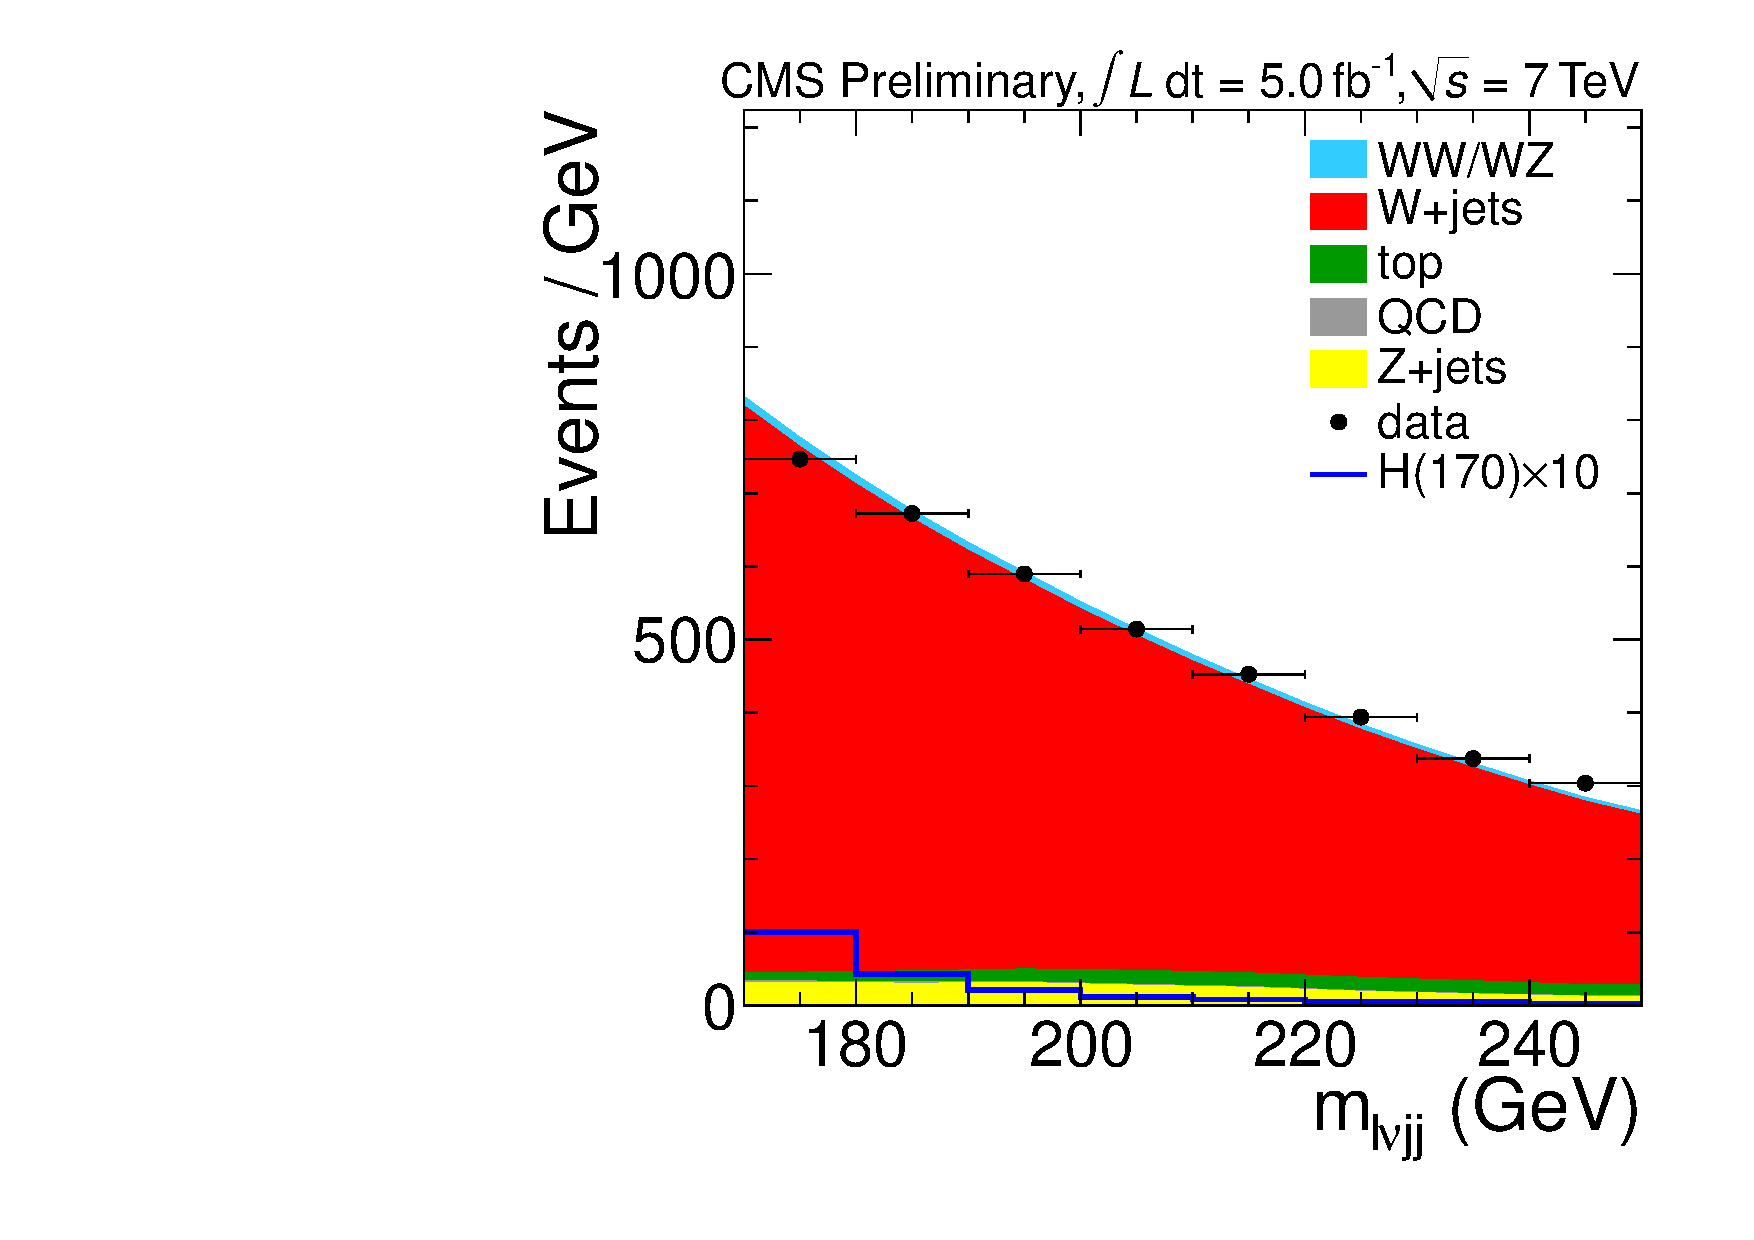
\includegraphics[width=0.3\textwidth]{plots/2012_FOURBSHAPES/H170_Mlvjj_Muon_2jets_Stacked}
    }
    \subfigure[]{
      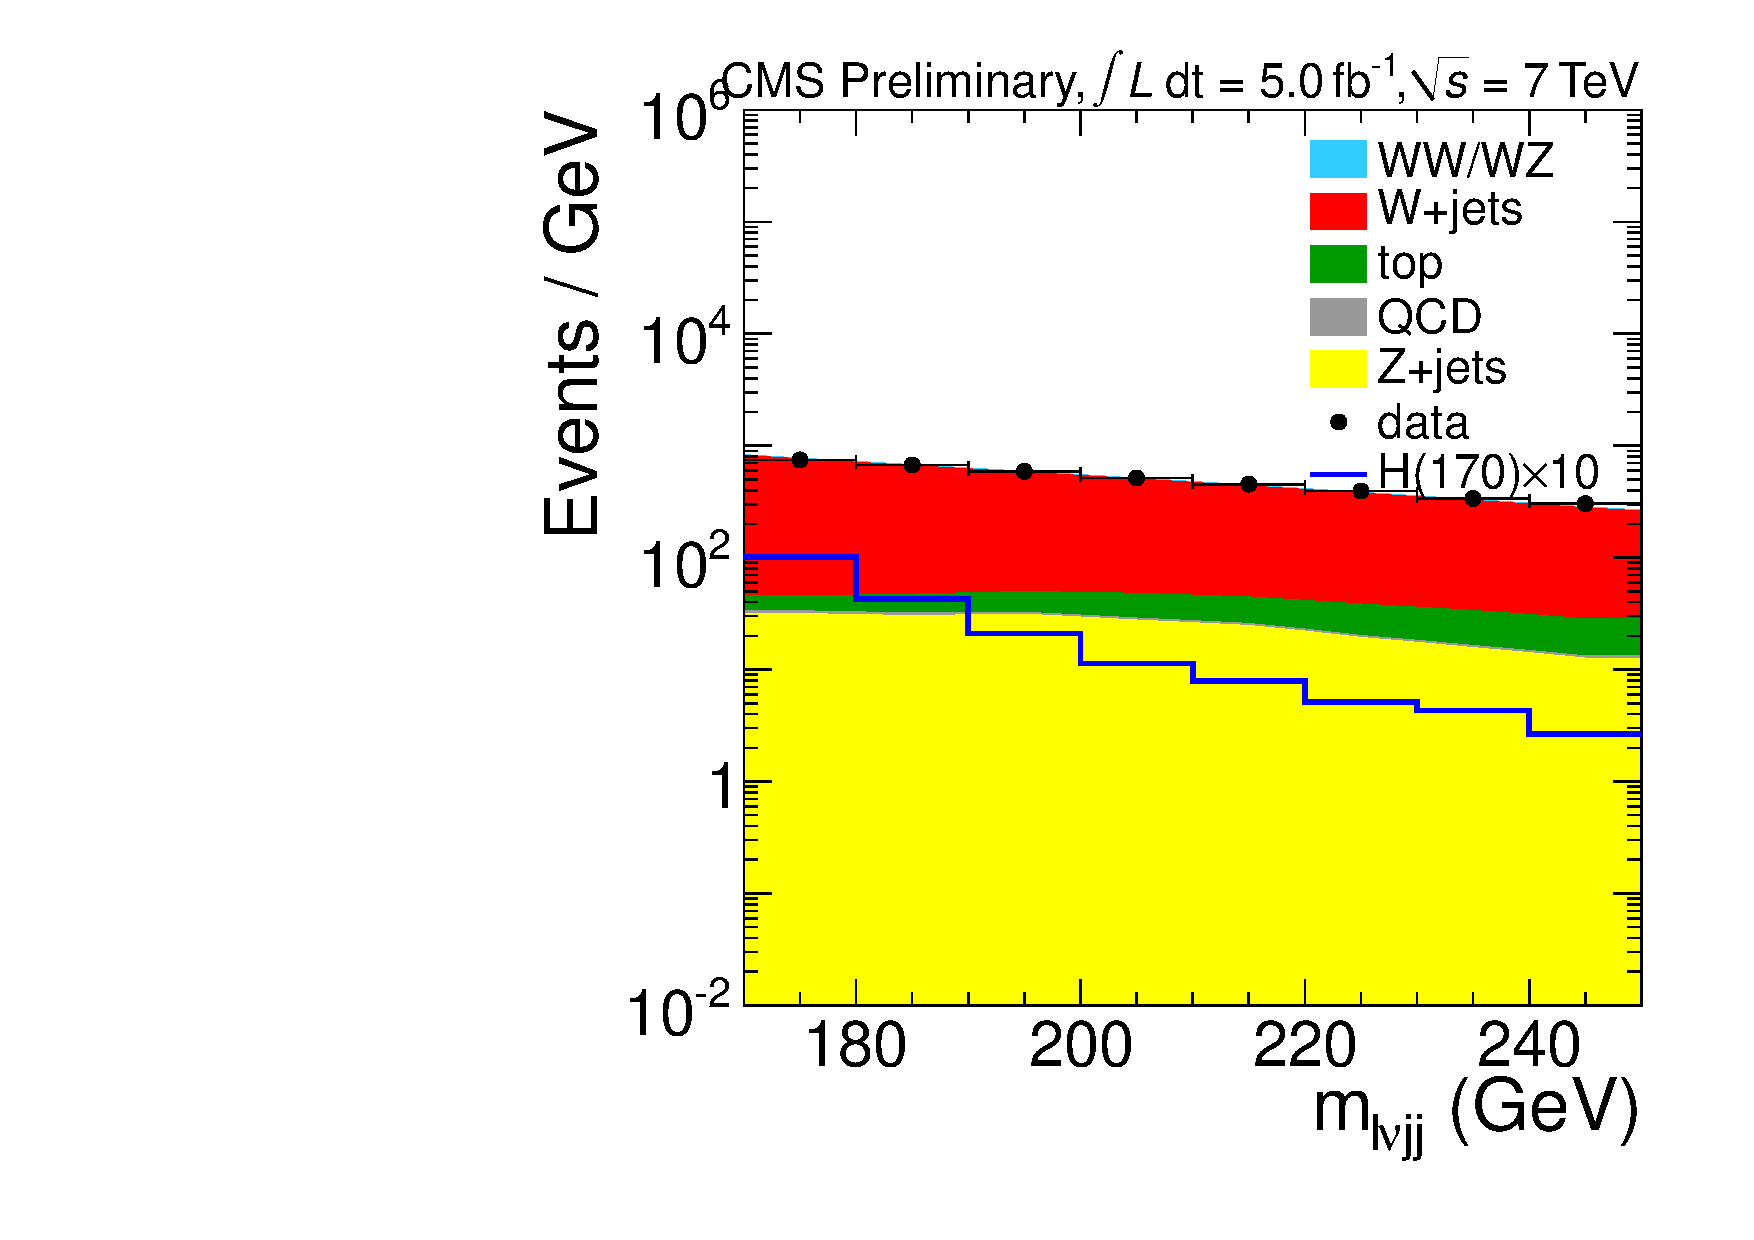
\includegraphics[width=0.3\textwidth]{plots/2012_FOURBSHAPES/H170_Mlvjj_Muon_2jets_Stacked_log}
    }
    \subfigure[]{
      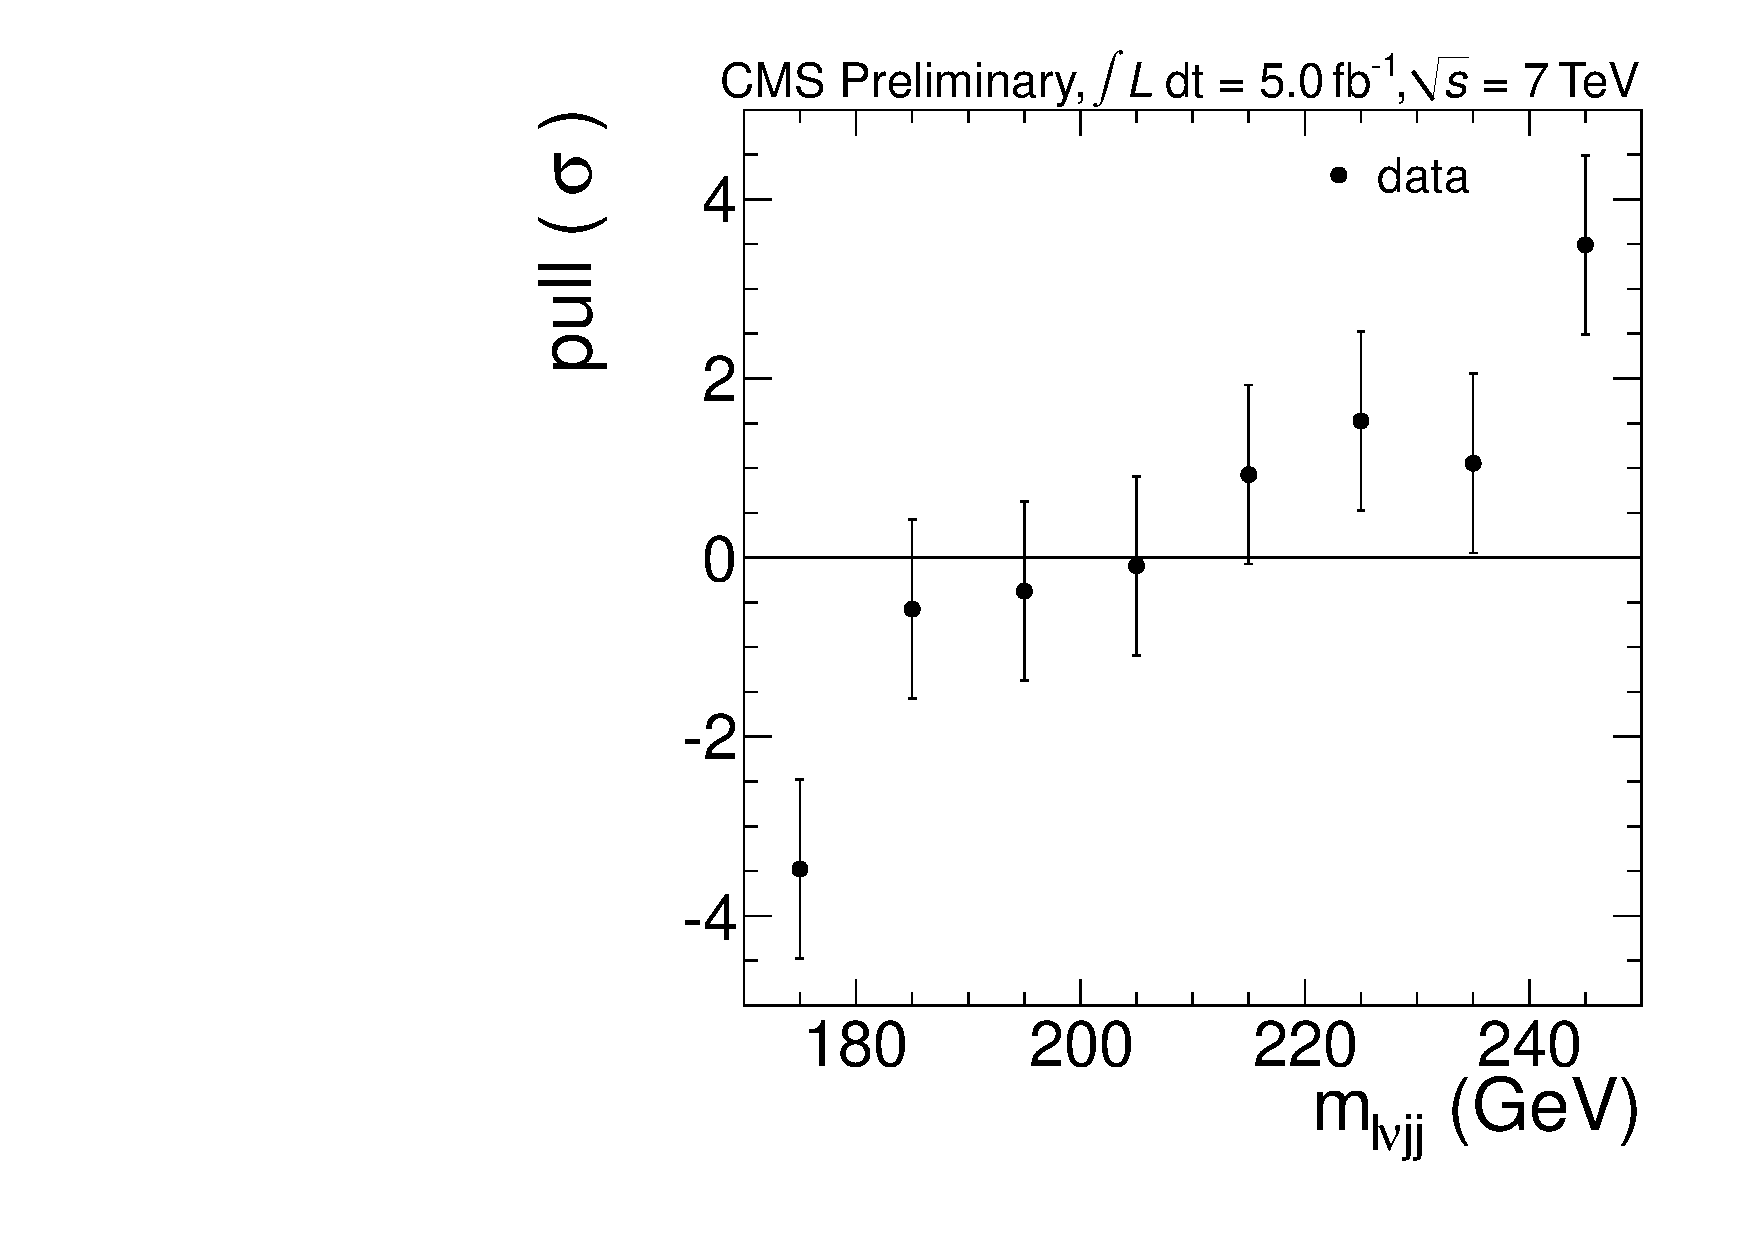
\includegraphics[width=0.3\textwidth]{plots/2012_FOURBSHAPES/H170_Mlvjj_Muon_2jets_Pull}
    }
    \vspace*{1mm} \\
    \subfigure[]{
        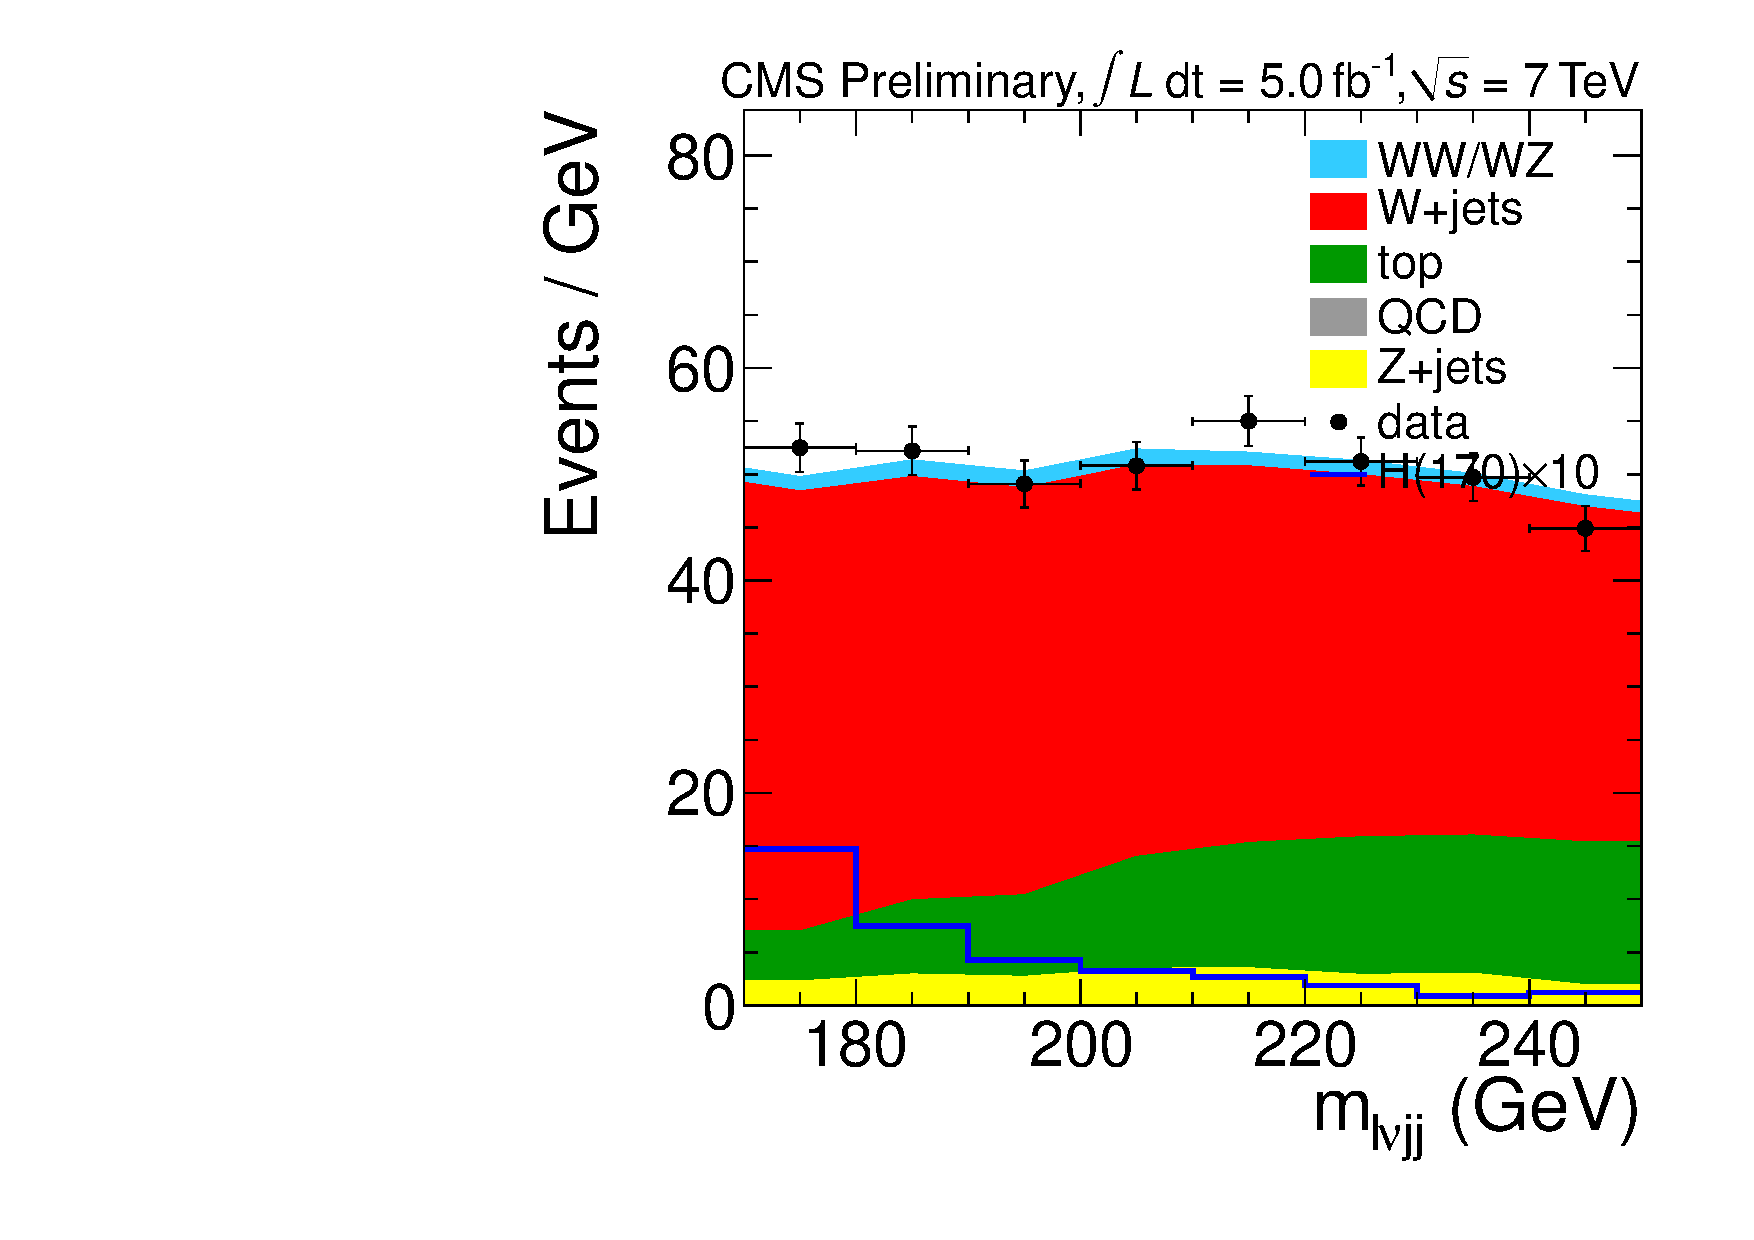
\includegraphics[width=0.3\textwidth]{plots/2012_FOURBSHAPES/H170_Mlvjj_Muon_3jets_Stacked}
    }
    \subfigure[]{
      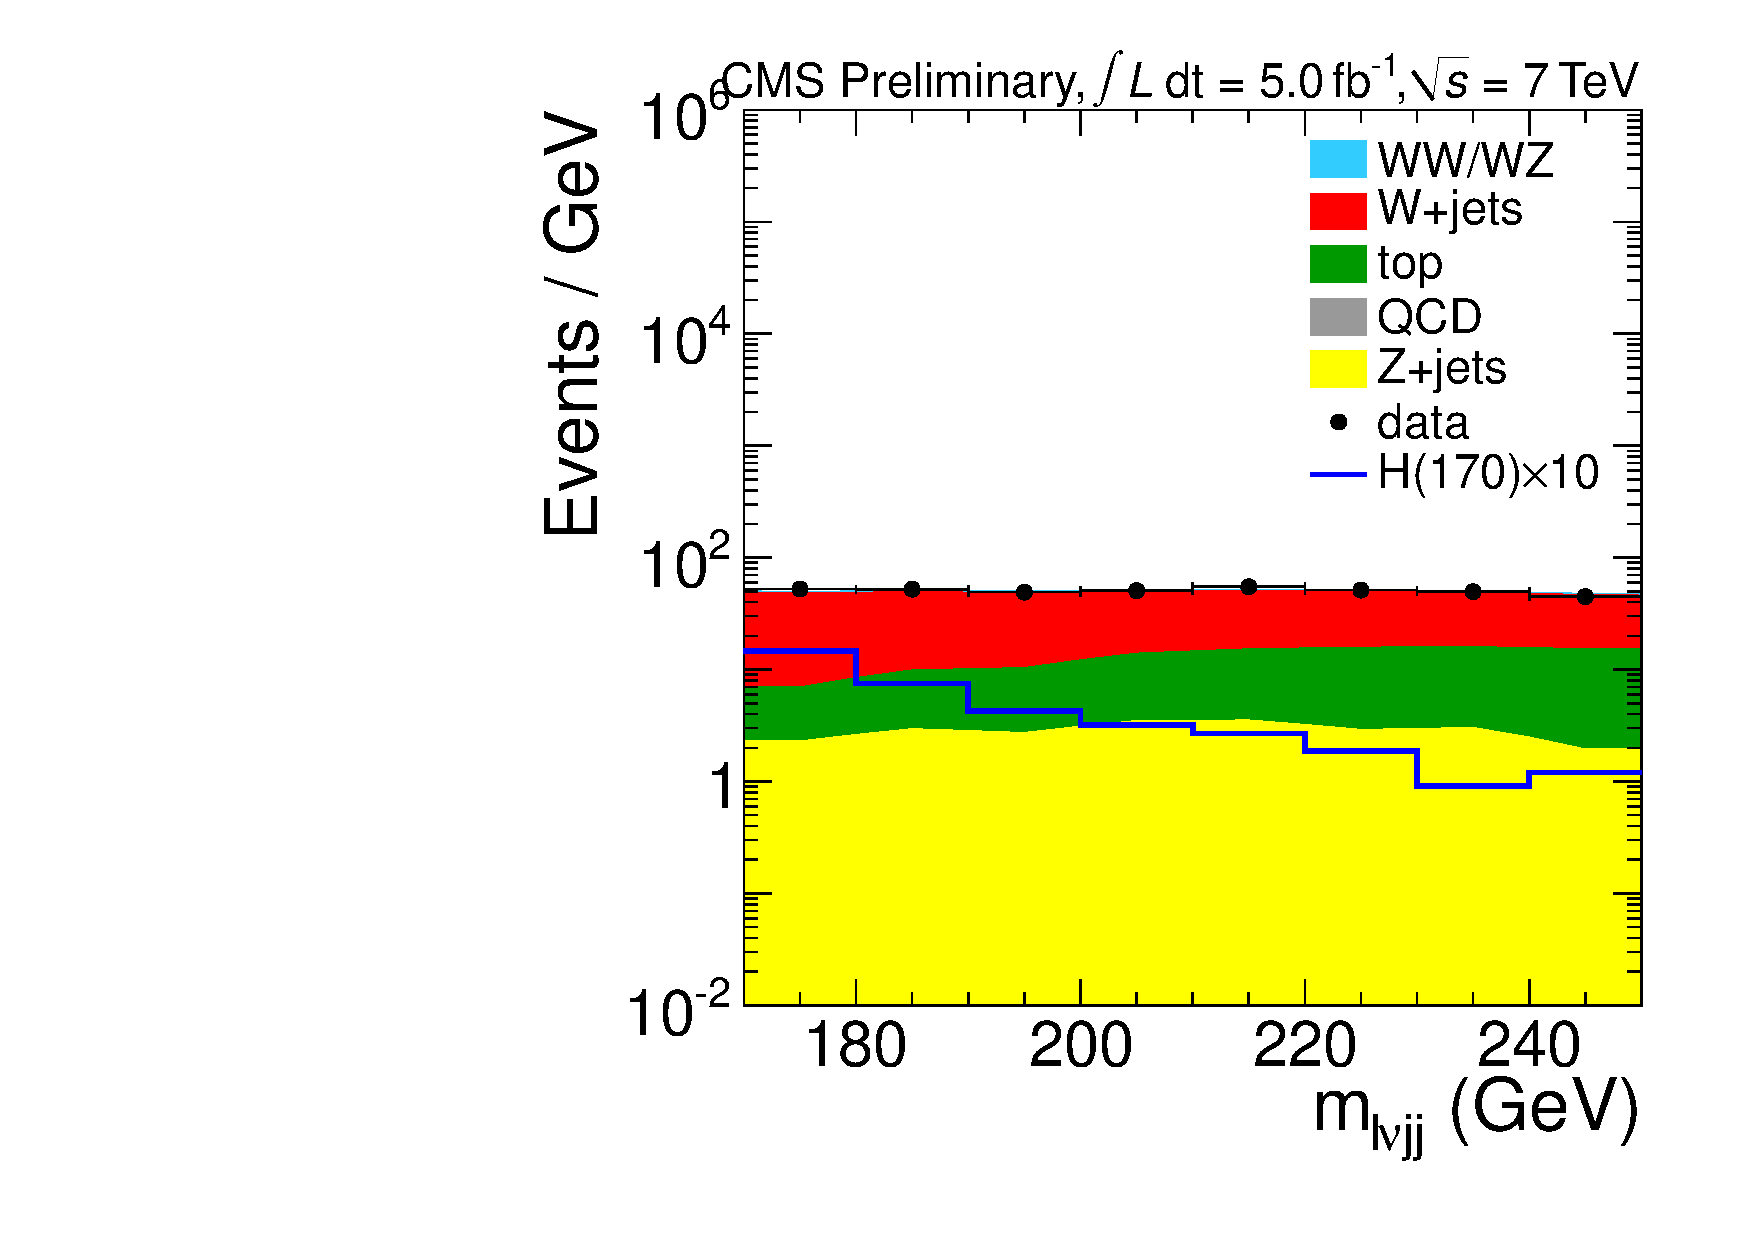
\includegraphics[width=0.3\textwidth]{plots/2012_FOURBSHAPES/H170_Mlvjj_Muon_3jets_Stacked_log}
    }
    \subfigure[]{
      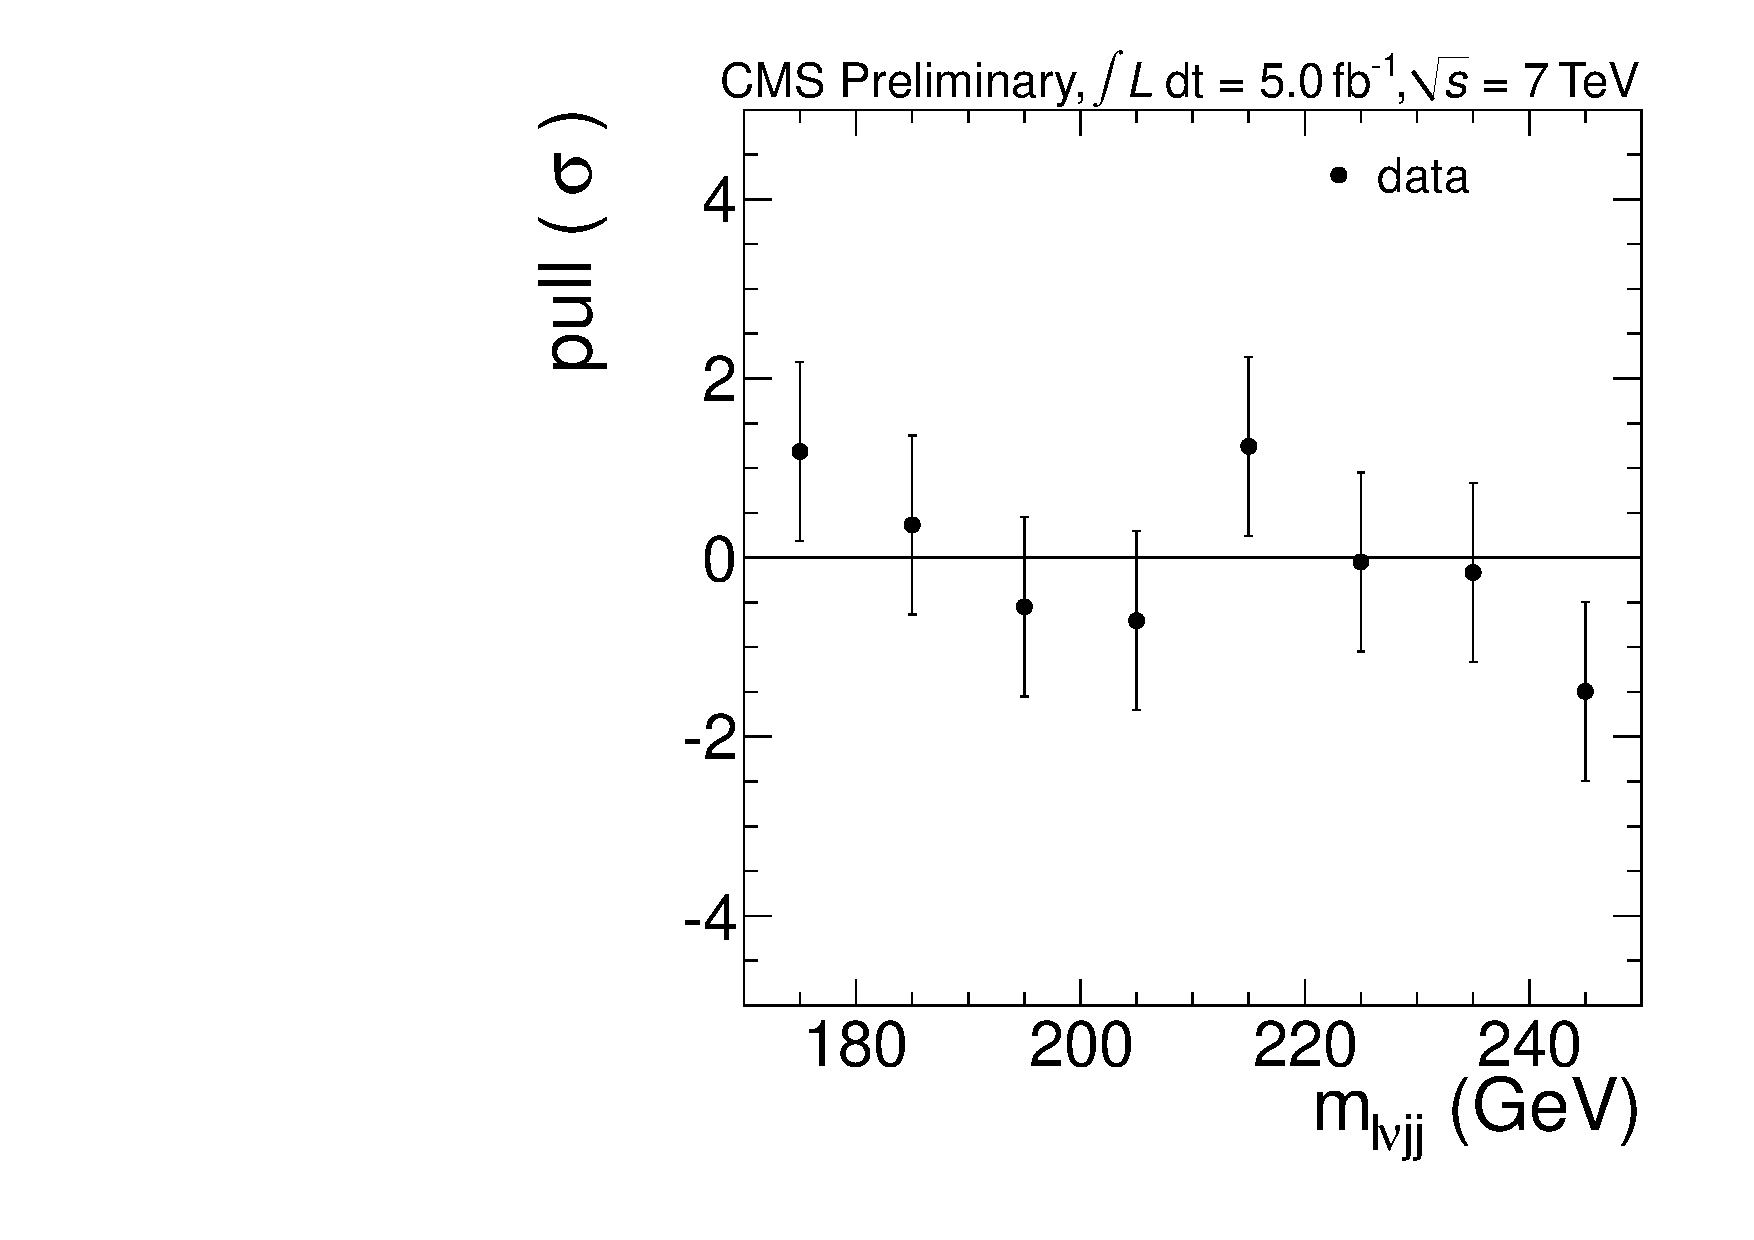
\includegraphics[width=0.3\textwidth]{plots/2012_FOURBSHAPES/H170_Mlvjj_Muon_3jets_Pull}
    }
    \vspace*{1mm} \\
    \subfigure[]{
        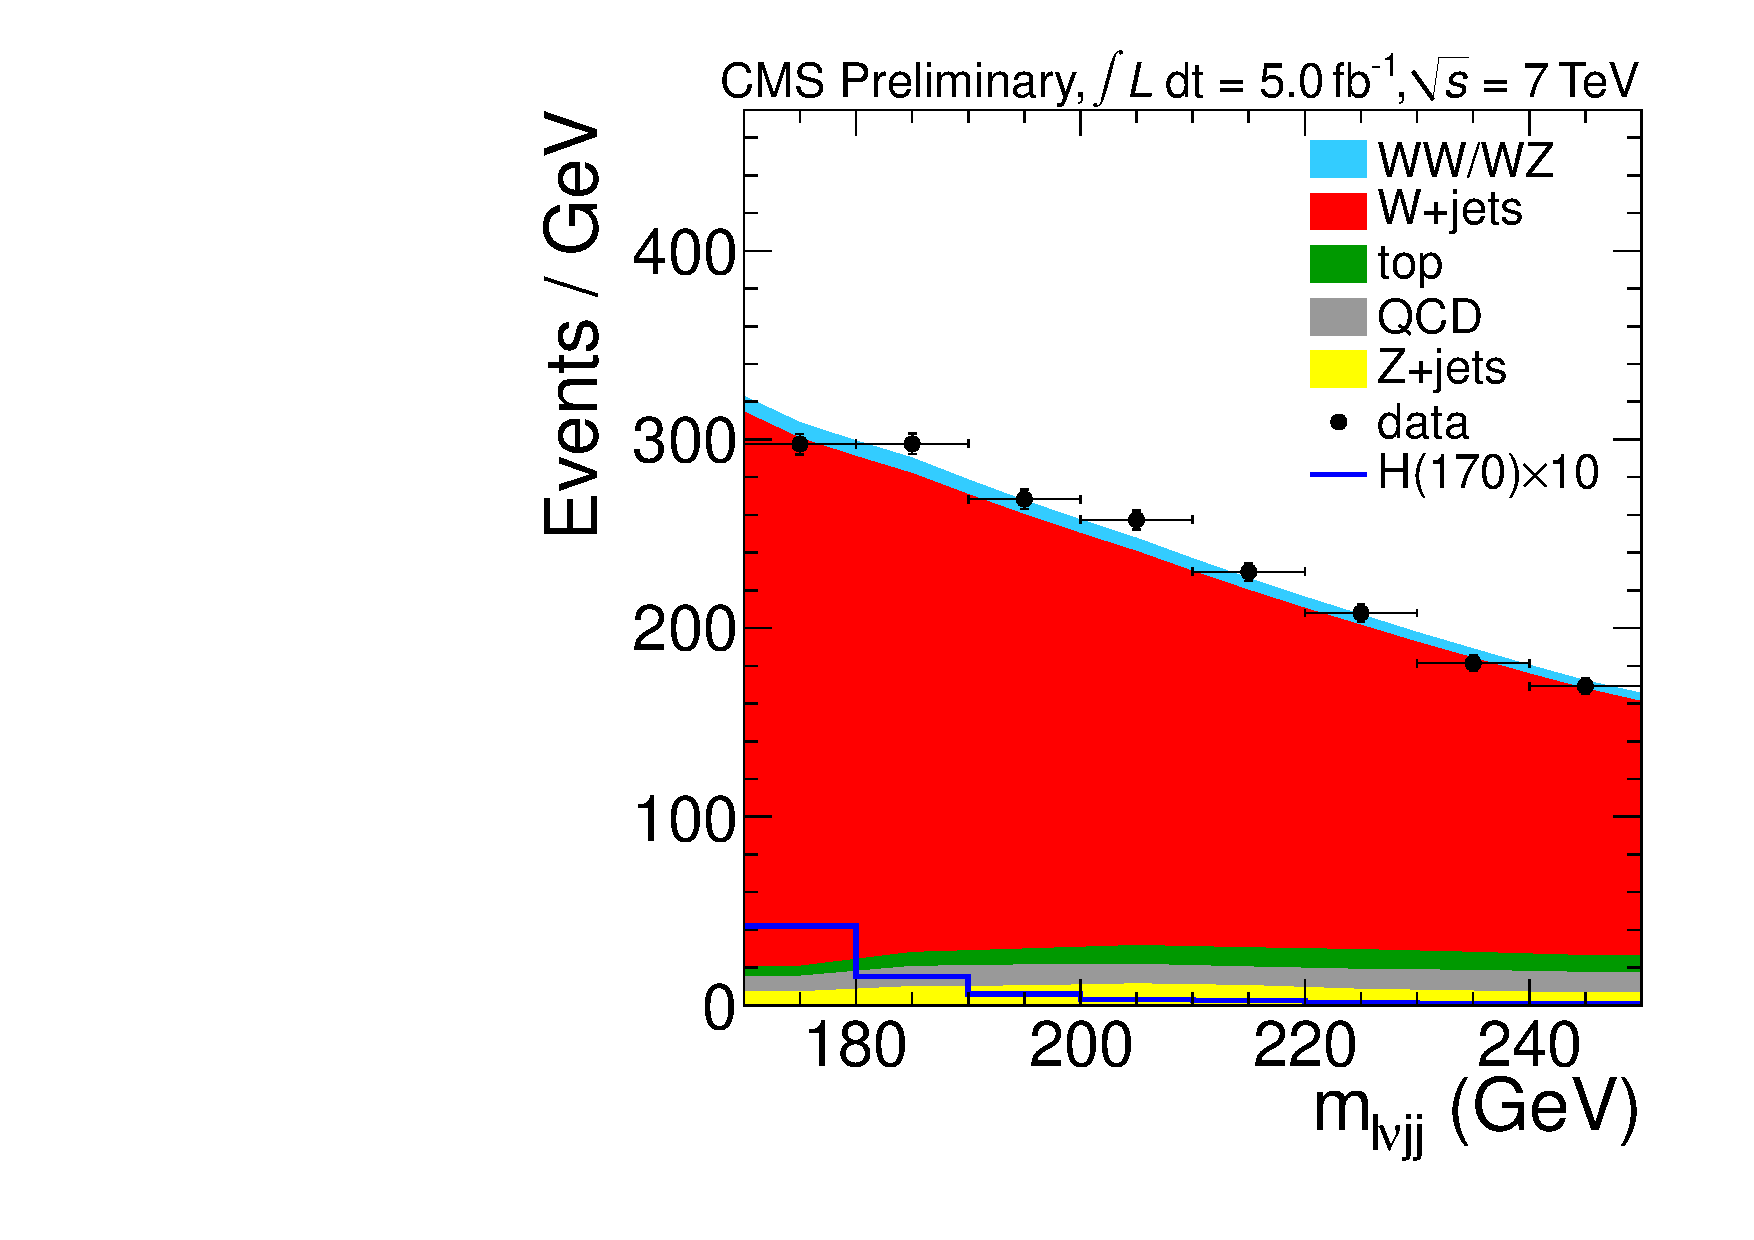
\includegraphics[width=0.3\textwidth]{plots/2012_FOURBSHAPES/H170_Mlvjj_Electron_2jets_Stacked}
    }
    \subfigure[]{
      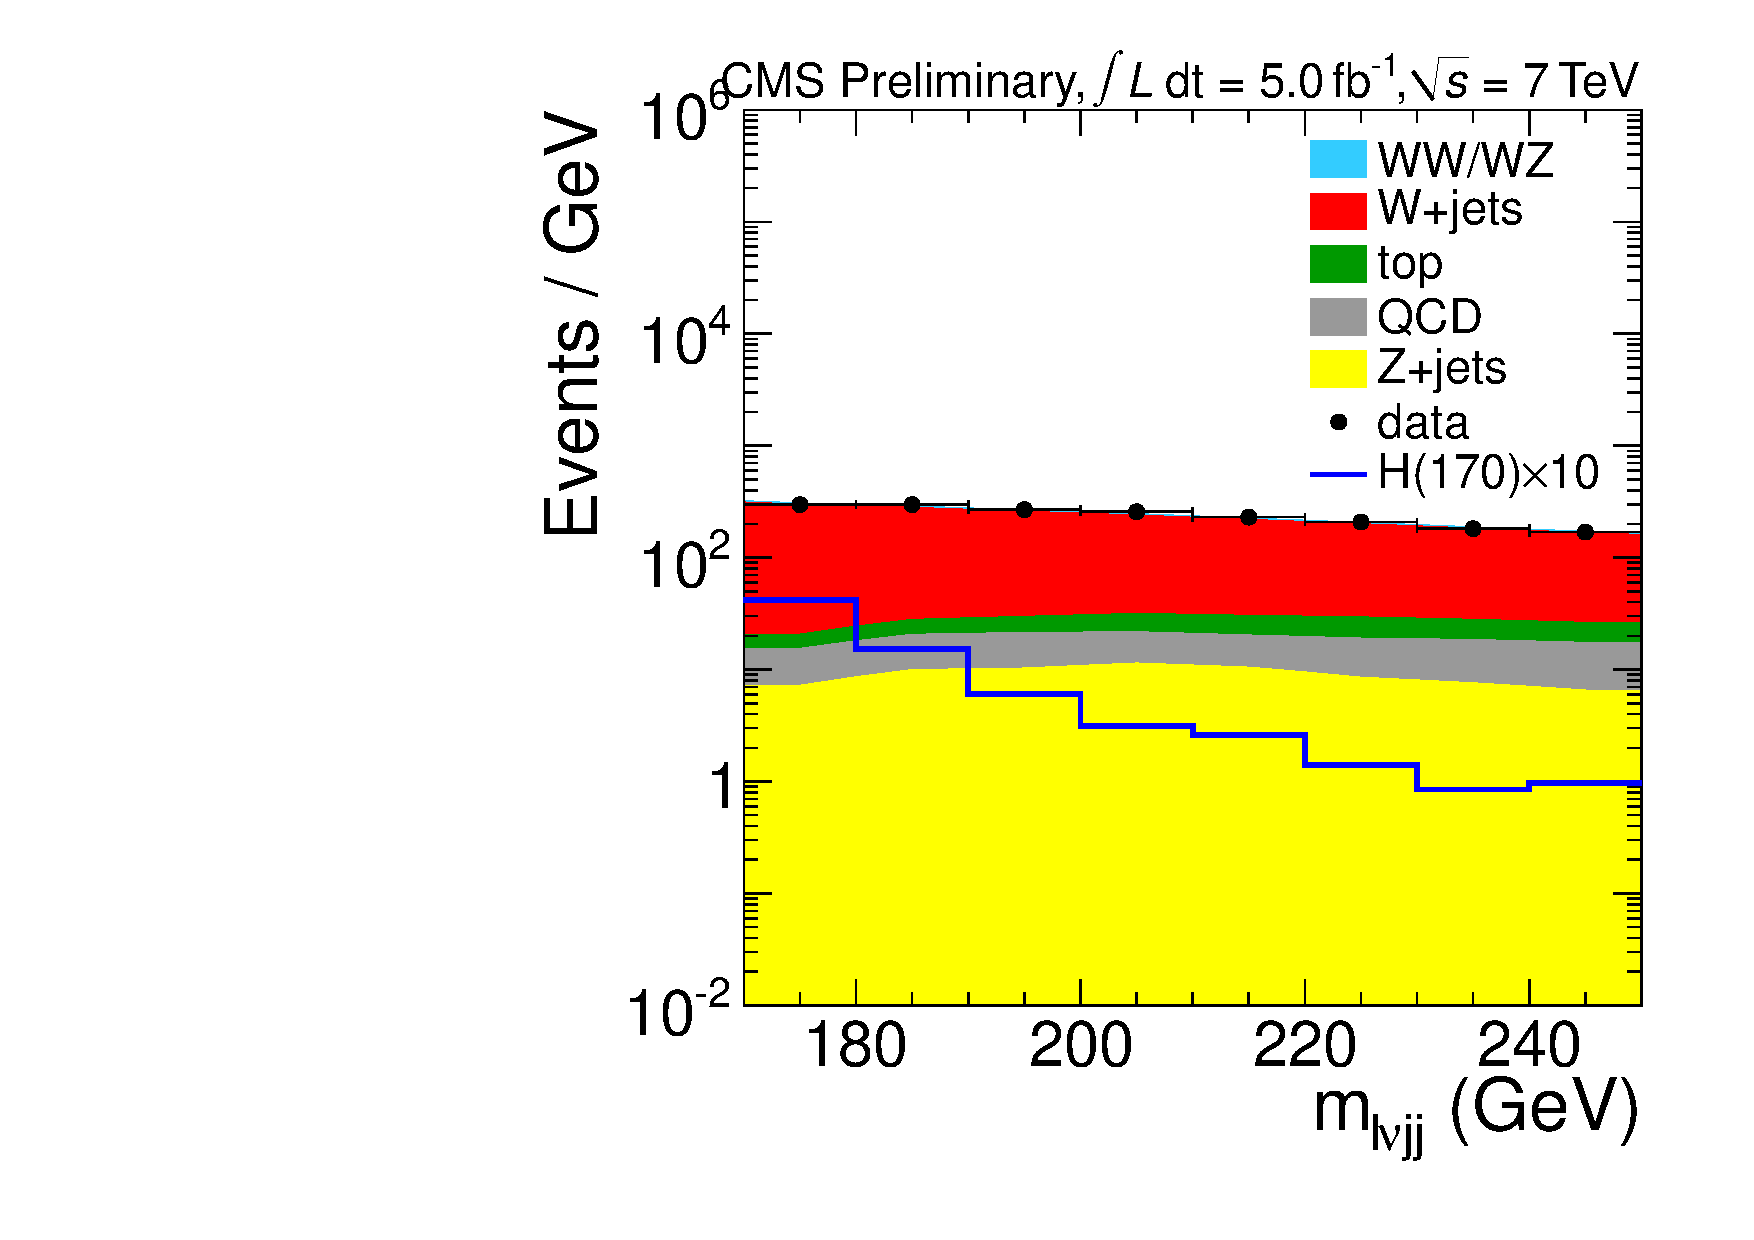
\includegraphics[width=0.3\textwidth]{plots/2012_FOURBSHAPES/H170_Mlvjj_Electron_2jets_Stacked_log}
    }
    \subfigure[]{
      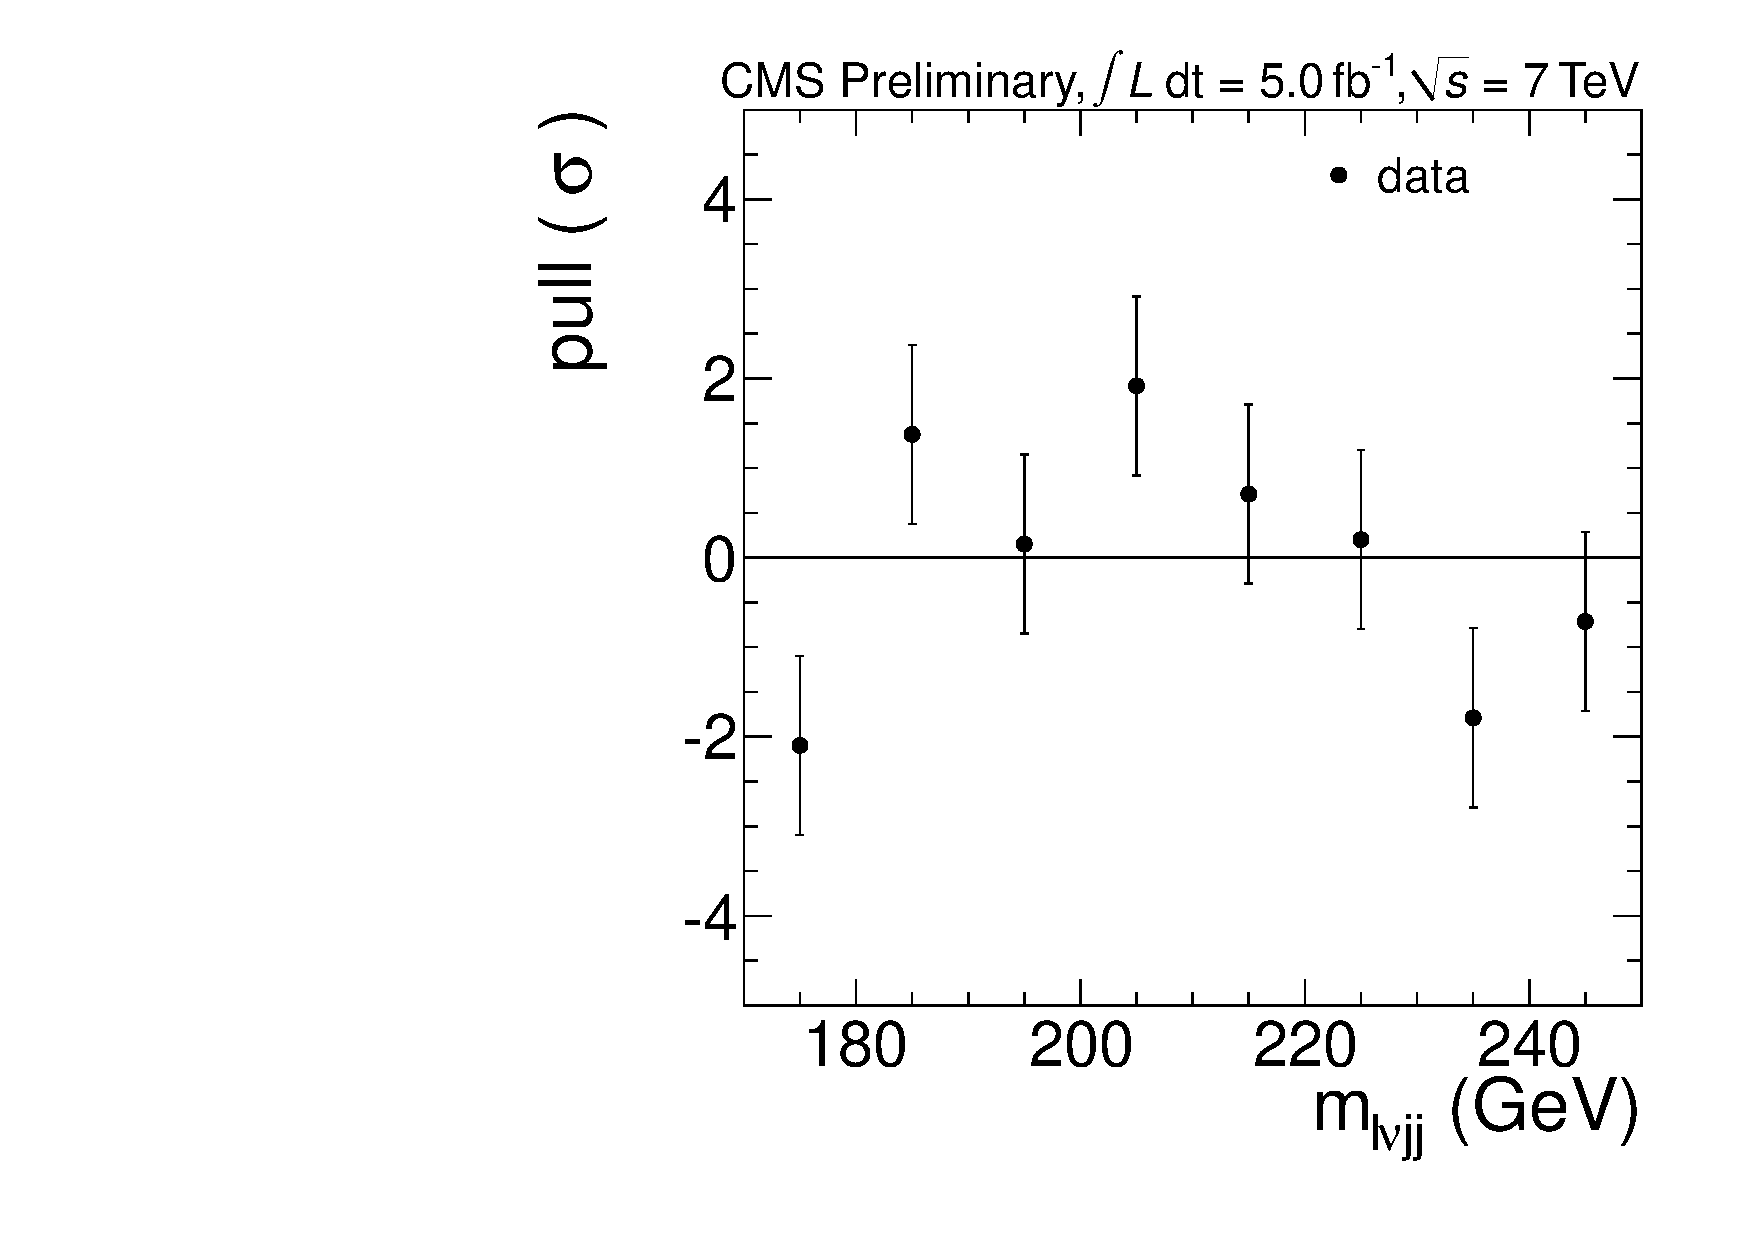
\includegraphics[width=0.3\textwidth]{plots/2012_FOURBSHAPES/H170_Mlvjj_Electron_2jets_Pull}
    }
    \vspace*{1mm} \\
    \subfigure[]{
        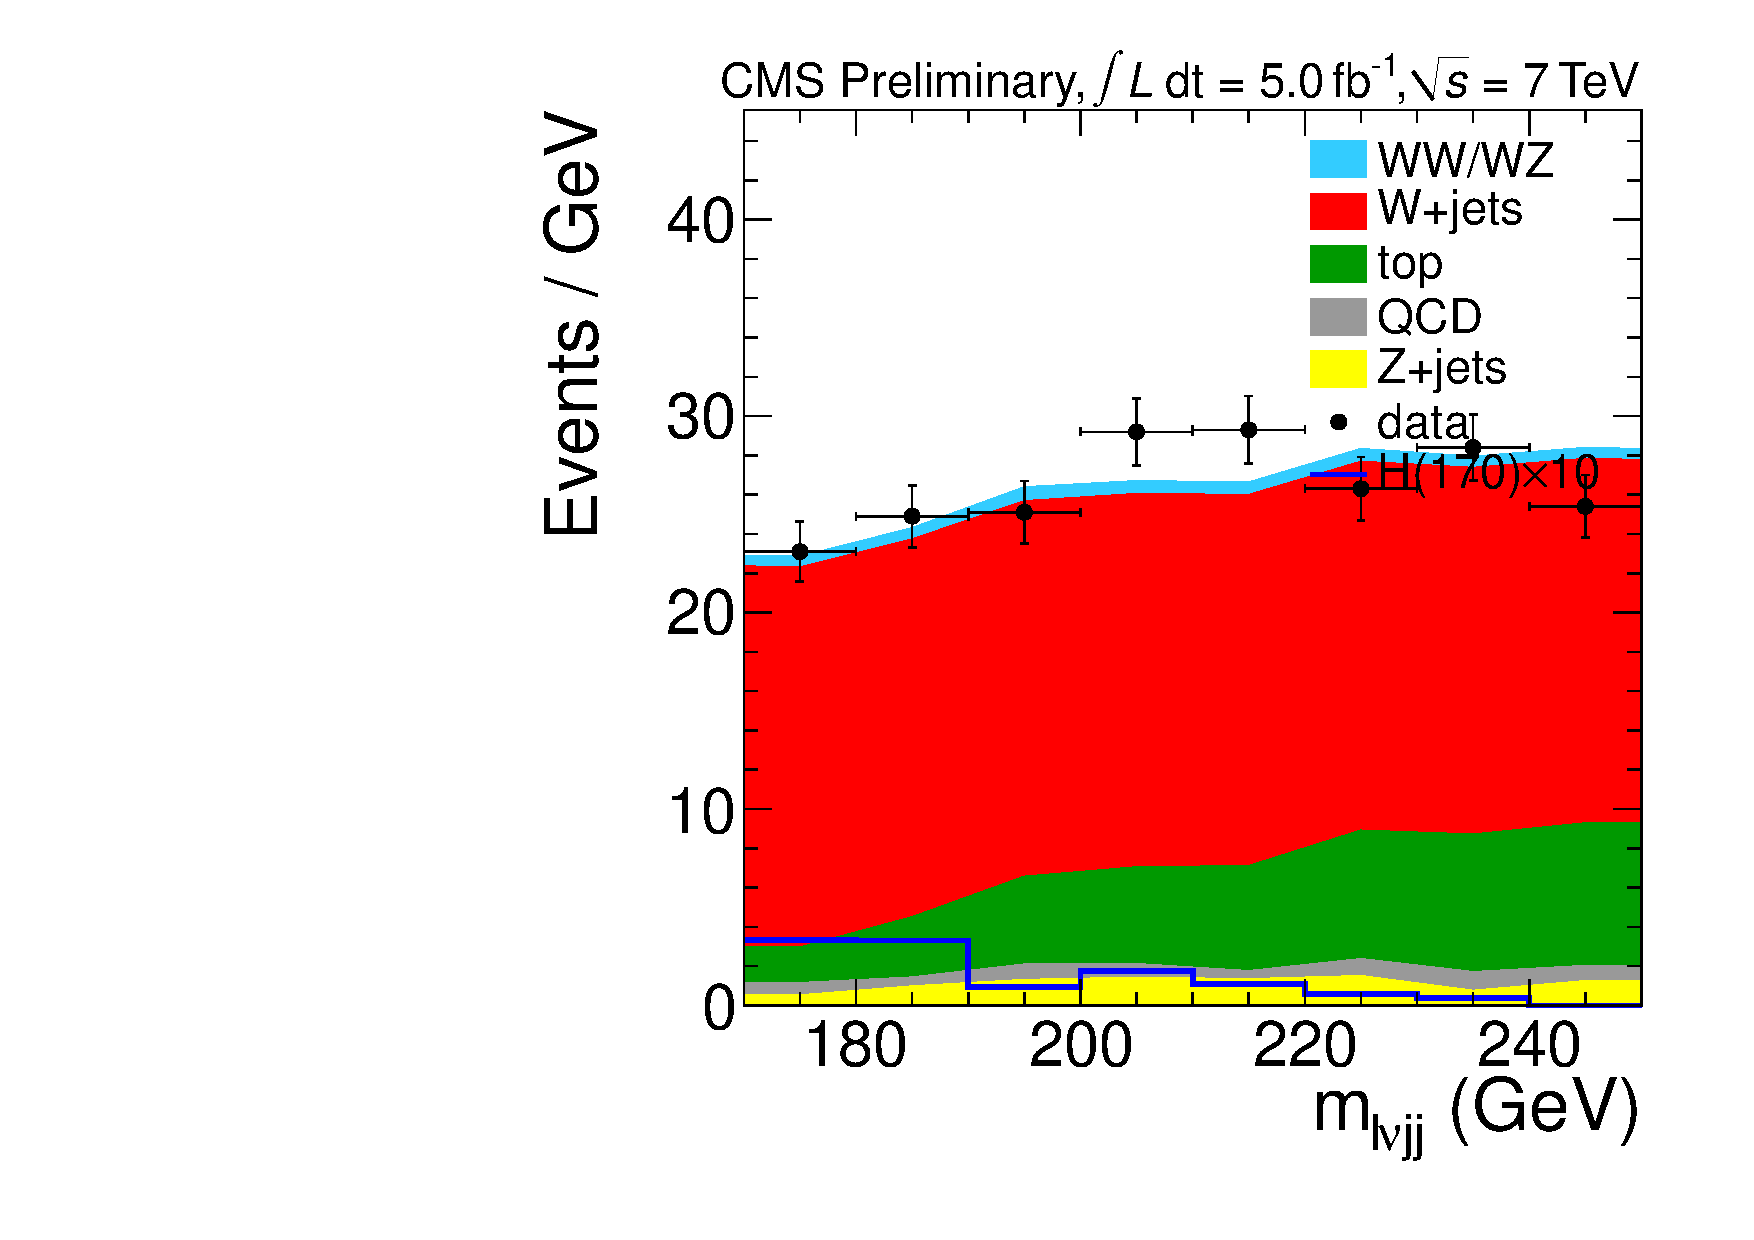
\includegraphics[width=0.3\textwidth]{plots/2012_FOURBSHAPES/H170_Mlvjj_Electron_3jets_Stacked}
    }
    \subfigure[]{
      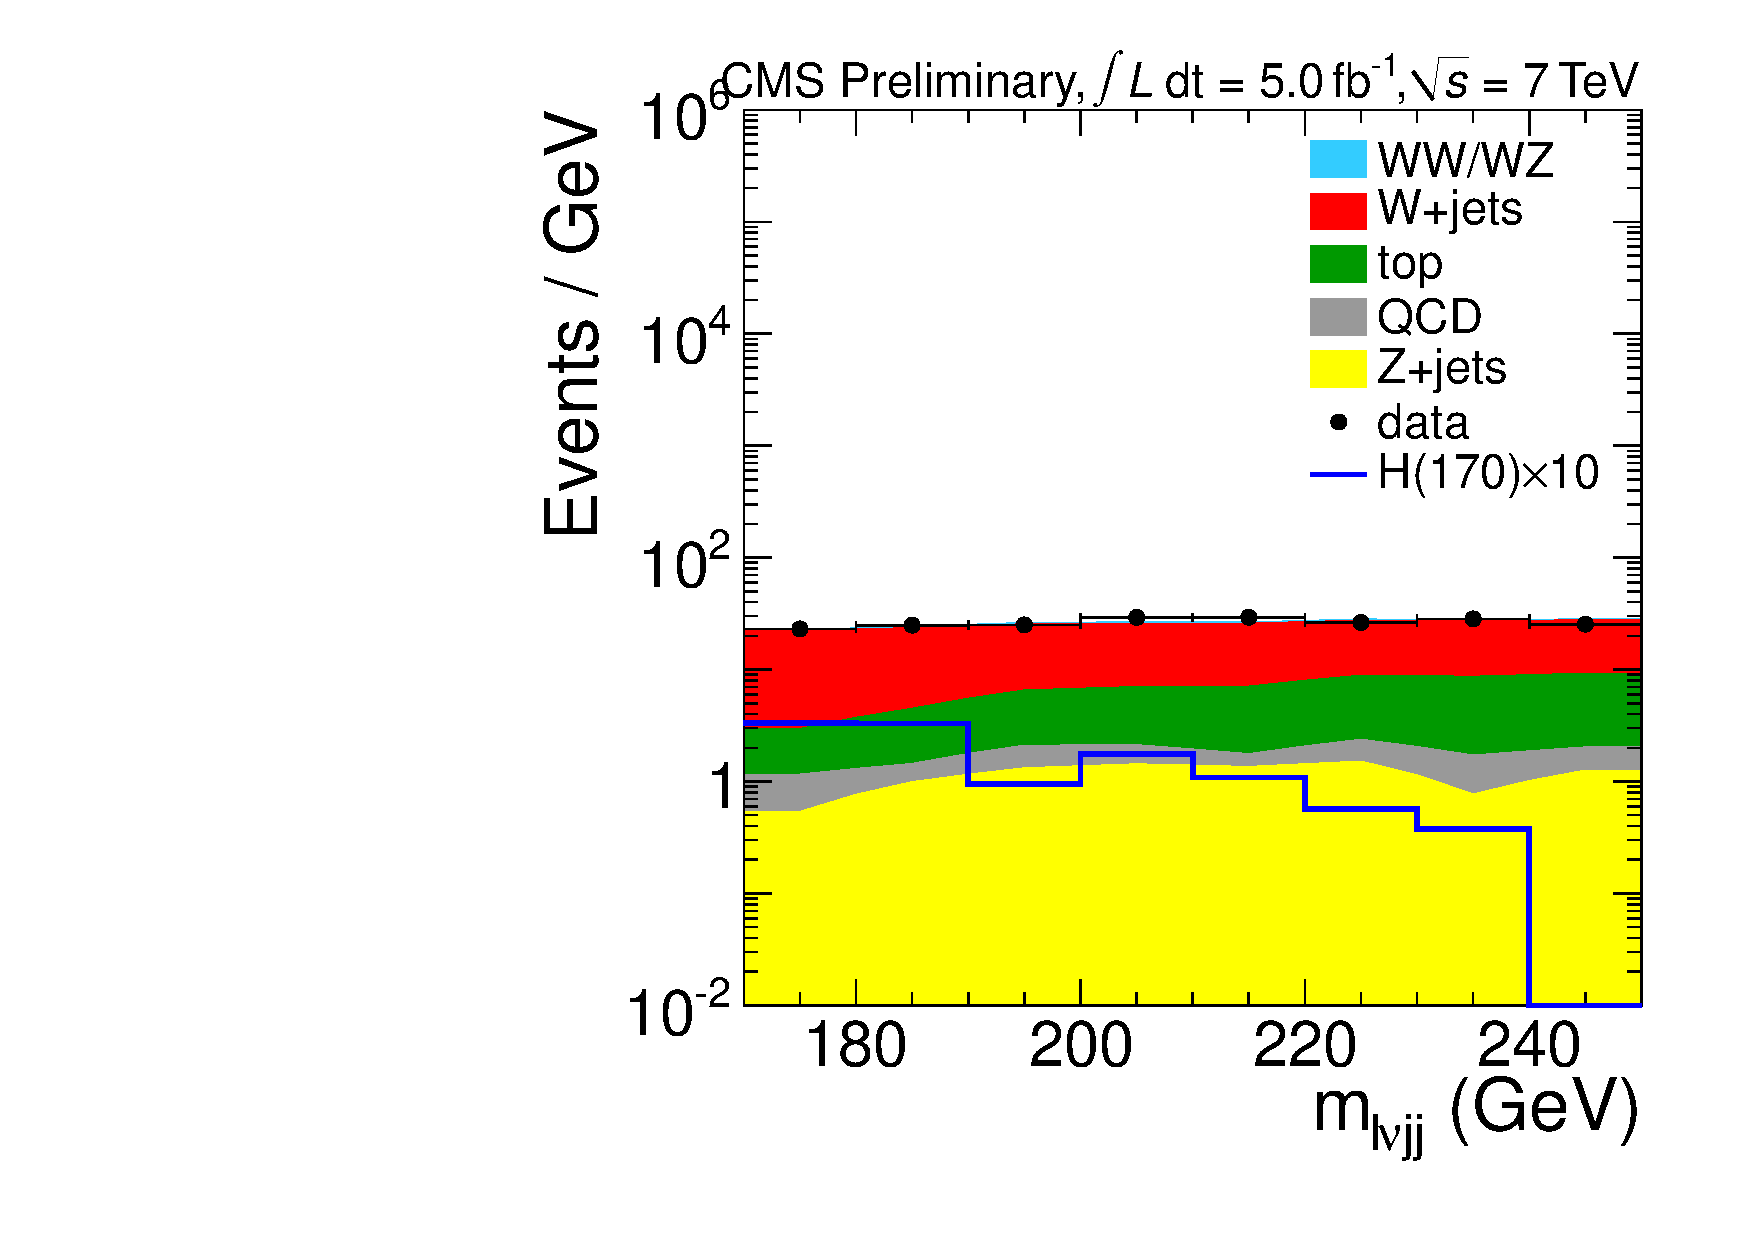
\includegraphics[width=0.3\textwidth]{plots/2012_FOURBSHAPES/H170_Mlvjj_Electron_3jets_Stacked_log}
    }
    \subfigure[]{
      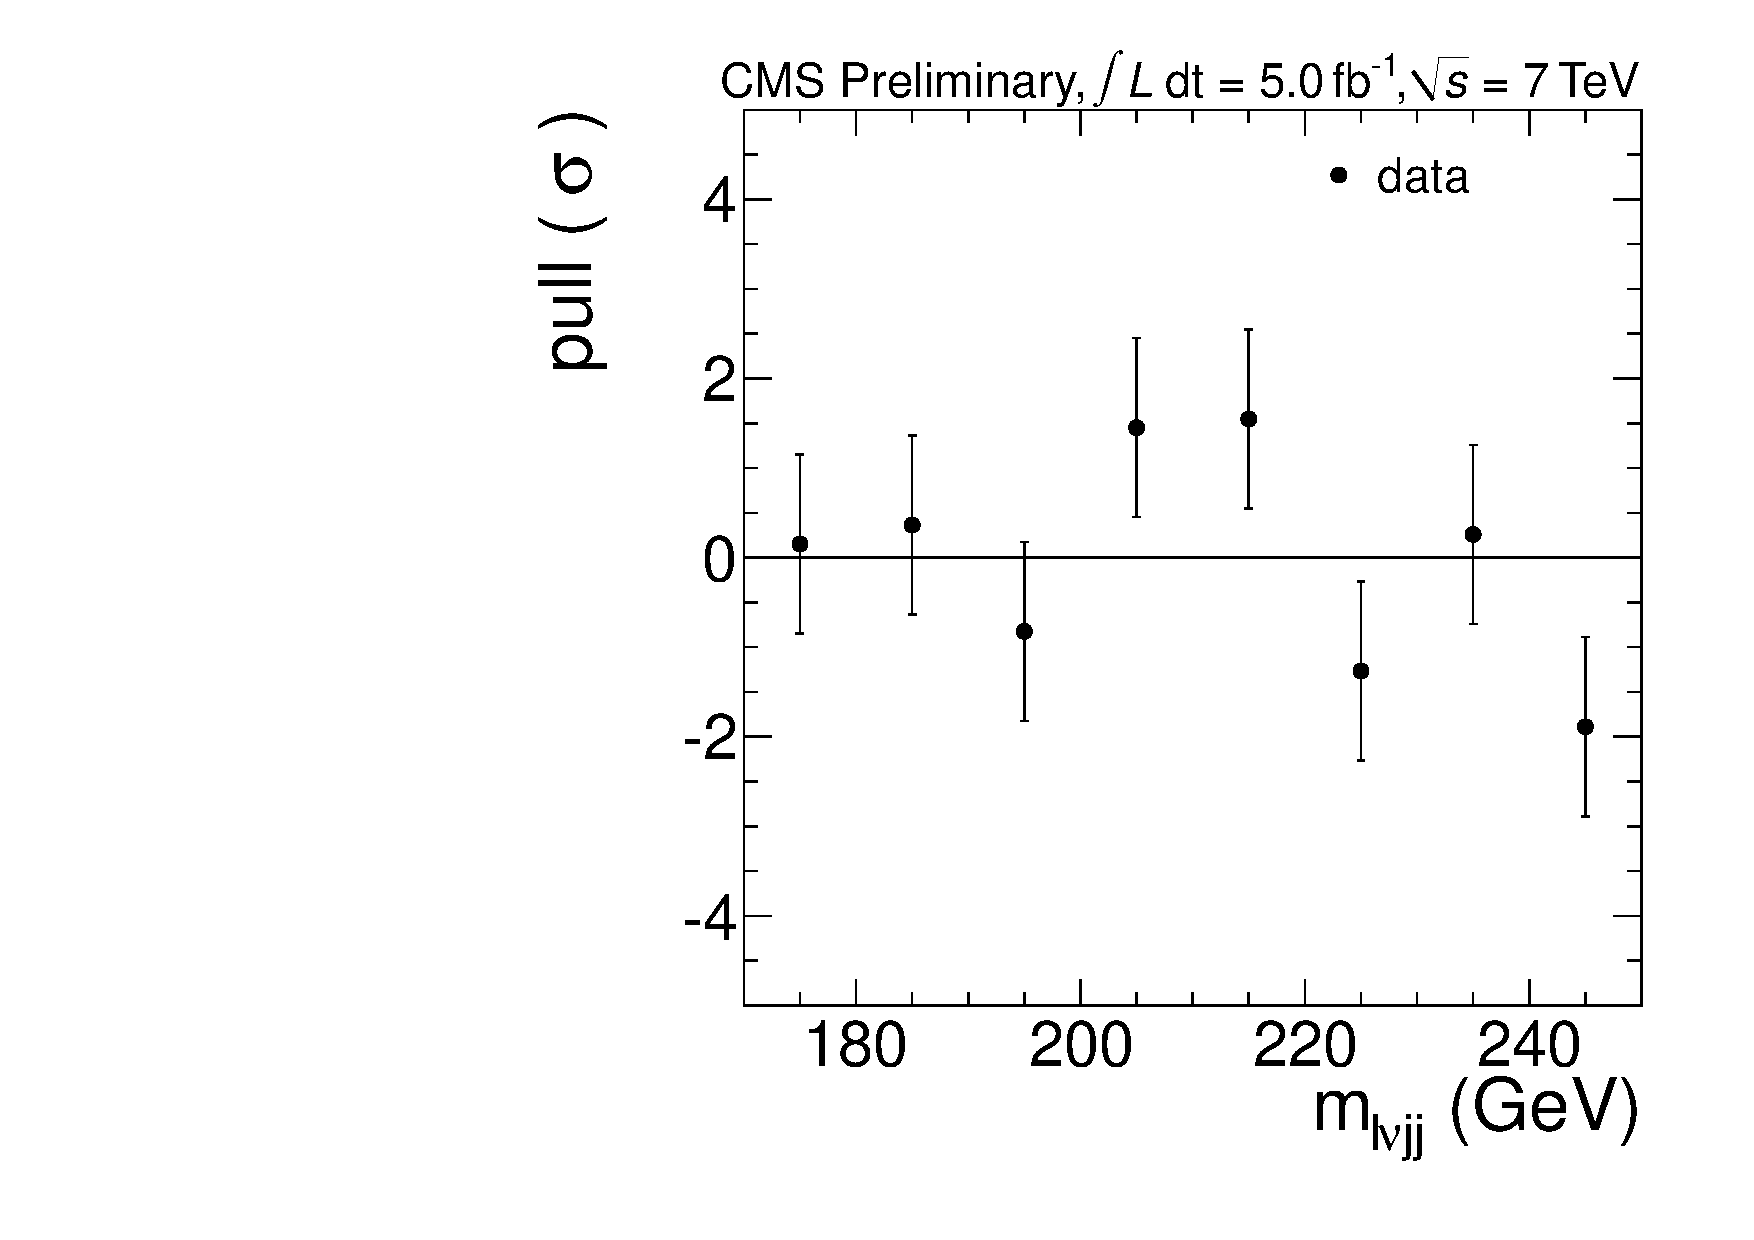
\includegraphics[width=0.3\textwidth]{plots/2012_FOURBSHAPES/H170_Mlvjj_Electron_3jets_Pull}
    }
    \caption{$M_H = 170$~GeV point. The distribution of the 4-body invariant mass $m_{\ell\nu jj}$ plotted on 
    linear (left) and log (center) scales. The pull distribution computed as 
    [(Data - Background)/ Background uncertainty] is shown on the right.
    The four rows correspond to muon 2-jets, muon 3-jets, electron 2-jets, 
    and electron 3-jets event categories, respectively. }
    \label{fig:mlnujj_mH170}
\end{figure}
%%%%%%%%%%%%%%%%%%%%
%%%%%%%%%%%%%%%%%%%%
%%%%%%%%%%%%%%%%%%%%
%  \begin{figure}[h!t]
%  \subfigure[]{
%      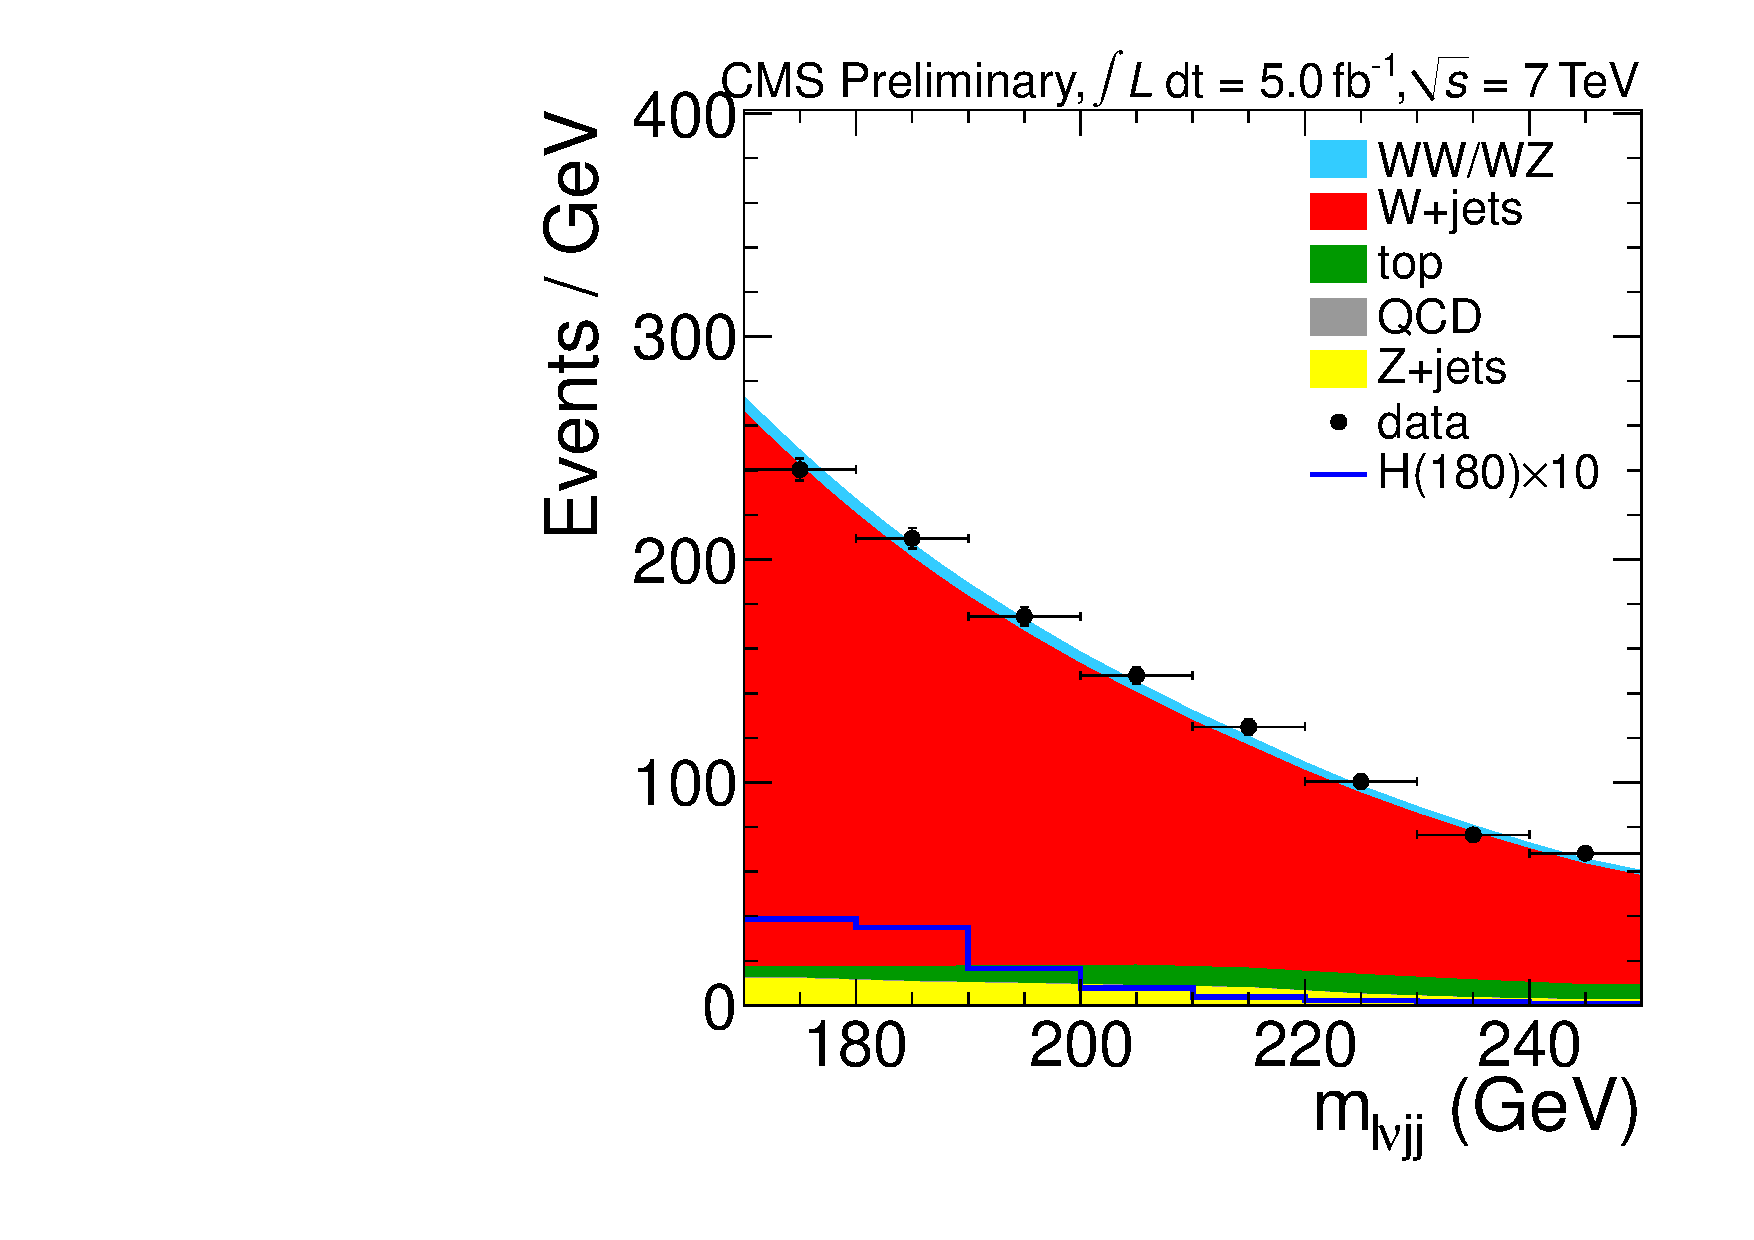
\includegraphics[width=0.3\textwidth]{plots/2012_FOURBSHAPES/H180_Mlvjj_Muon_2jets_Stacked}
%  }
%  \subfigure[]{
%    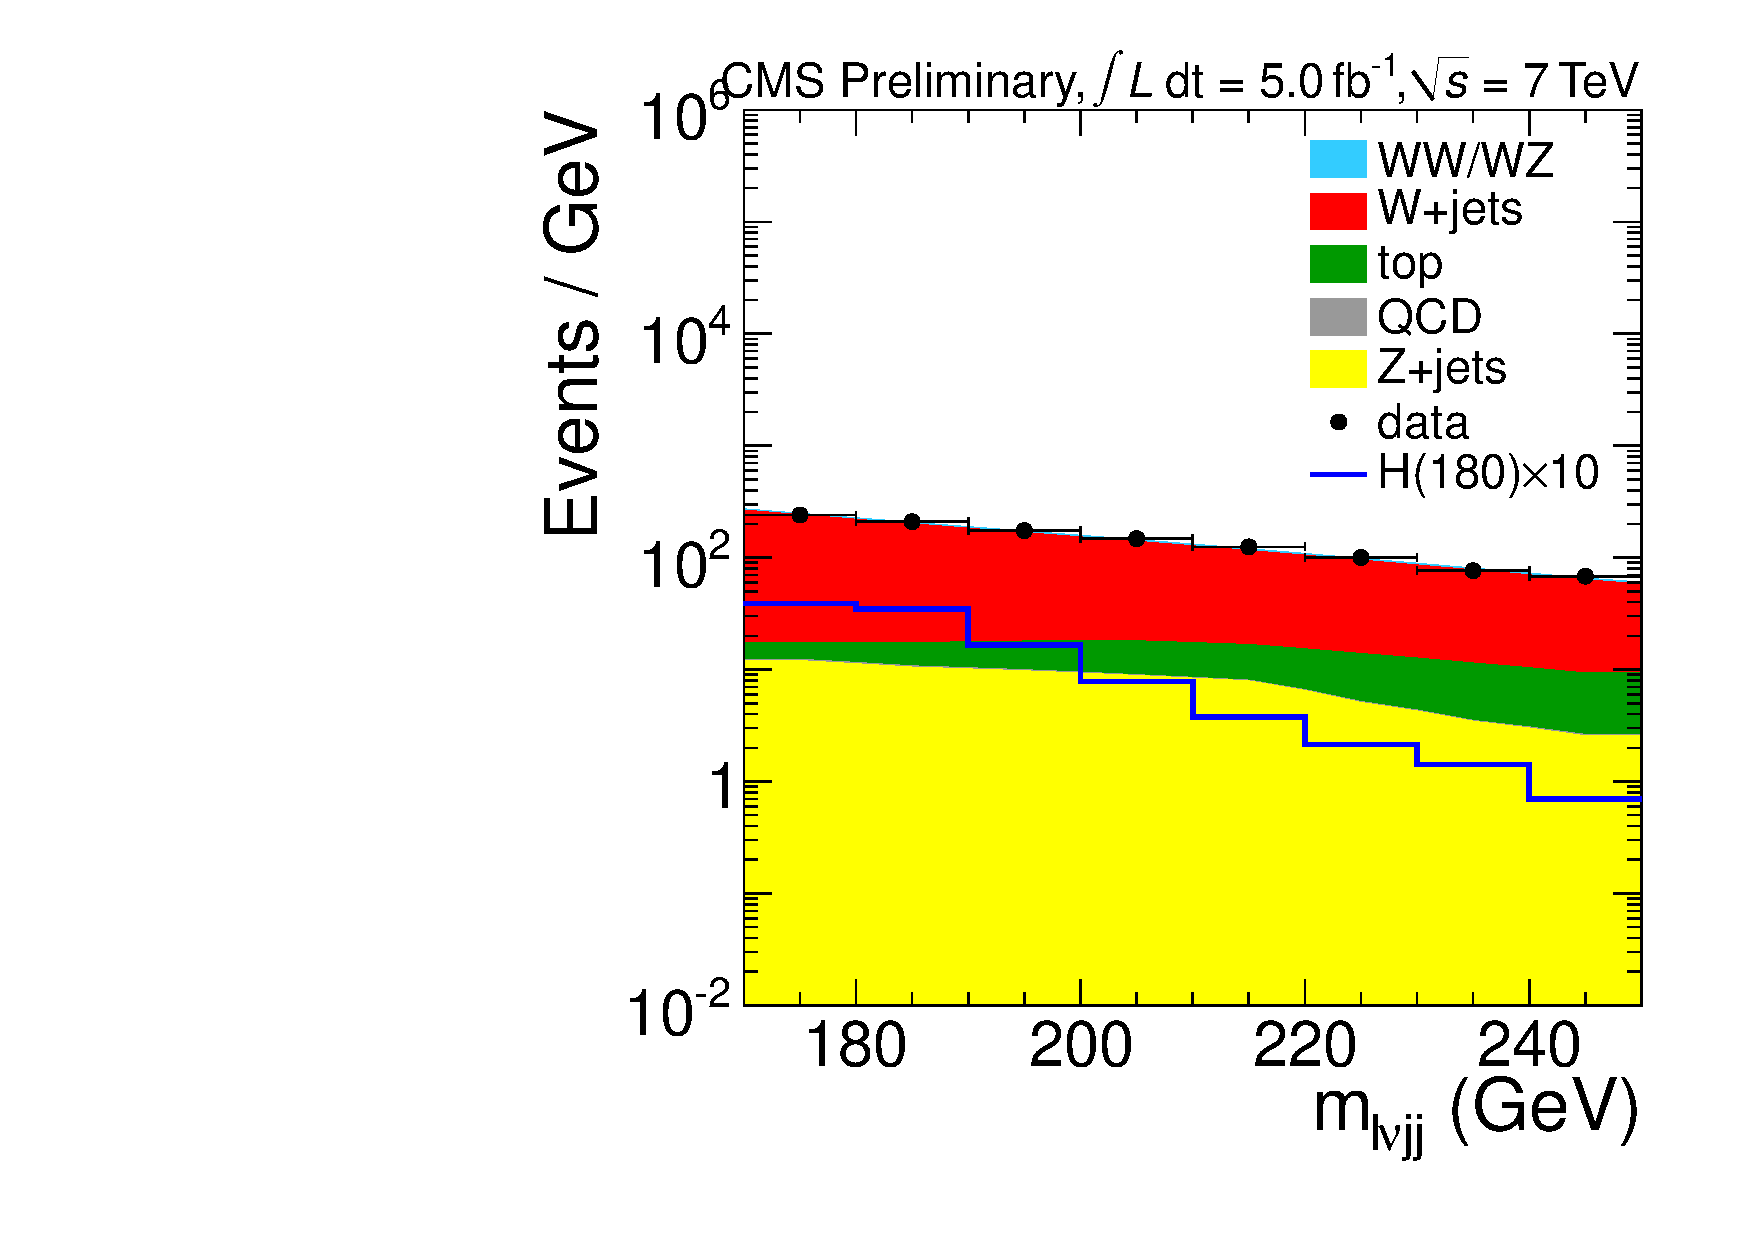
\includegraphics[width=0.3\textwidth]{plots/2012_FOURBSHAPES/H180_Mlvjj_Muon_2jets_Stacked_log}
%  }
%  \subfigure[]{
%    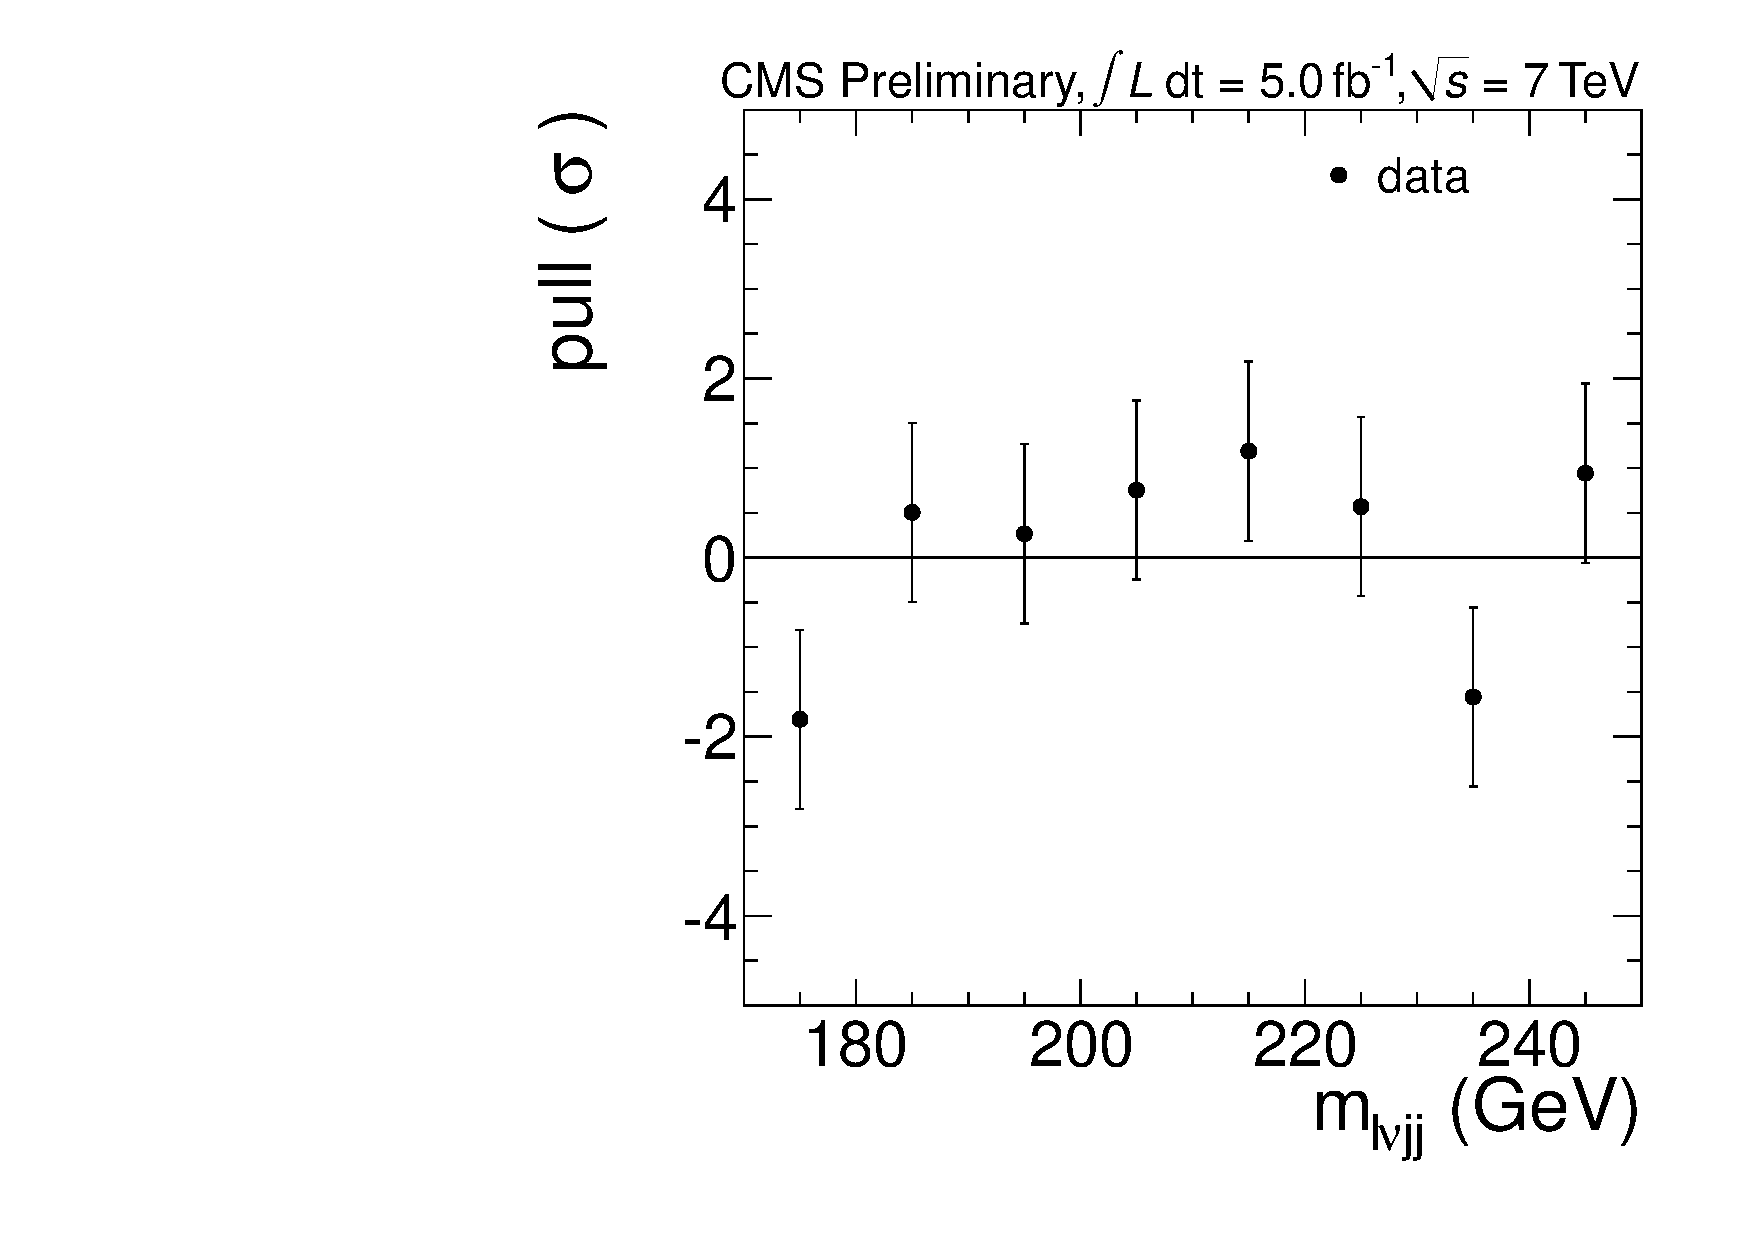
\includegraphics[width=0.3\textwidth]{plots/2012_FOURBSHAPES/H180_Mlvjj_Muon_2jets_Pull}
%  }
%  \vspace*{1mm} \\
%  \subfigure[]{
%      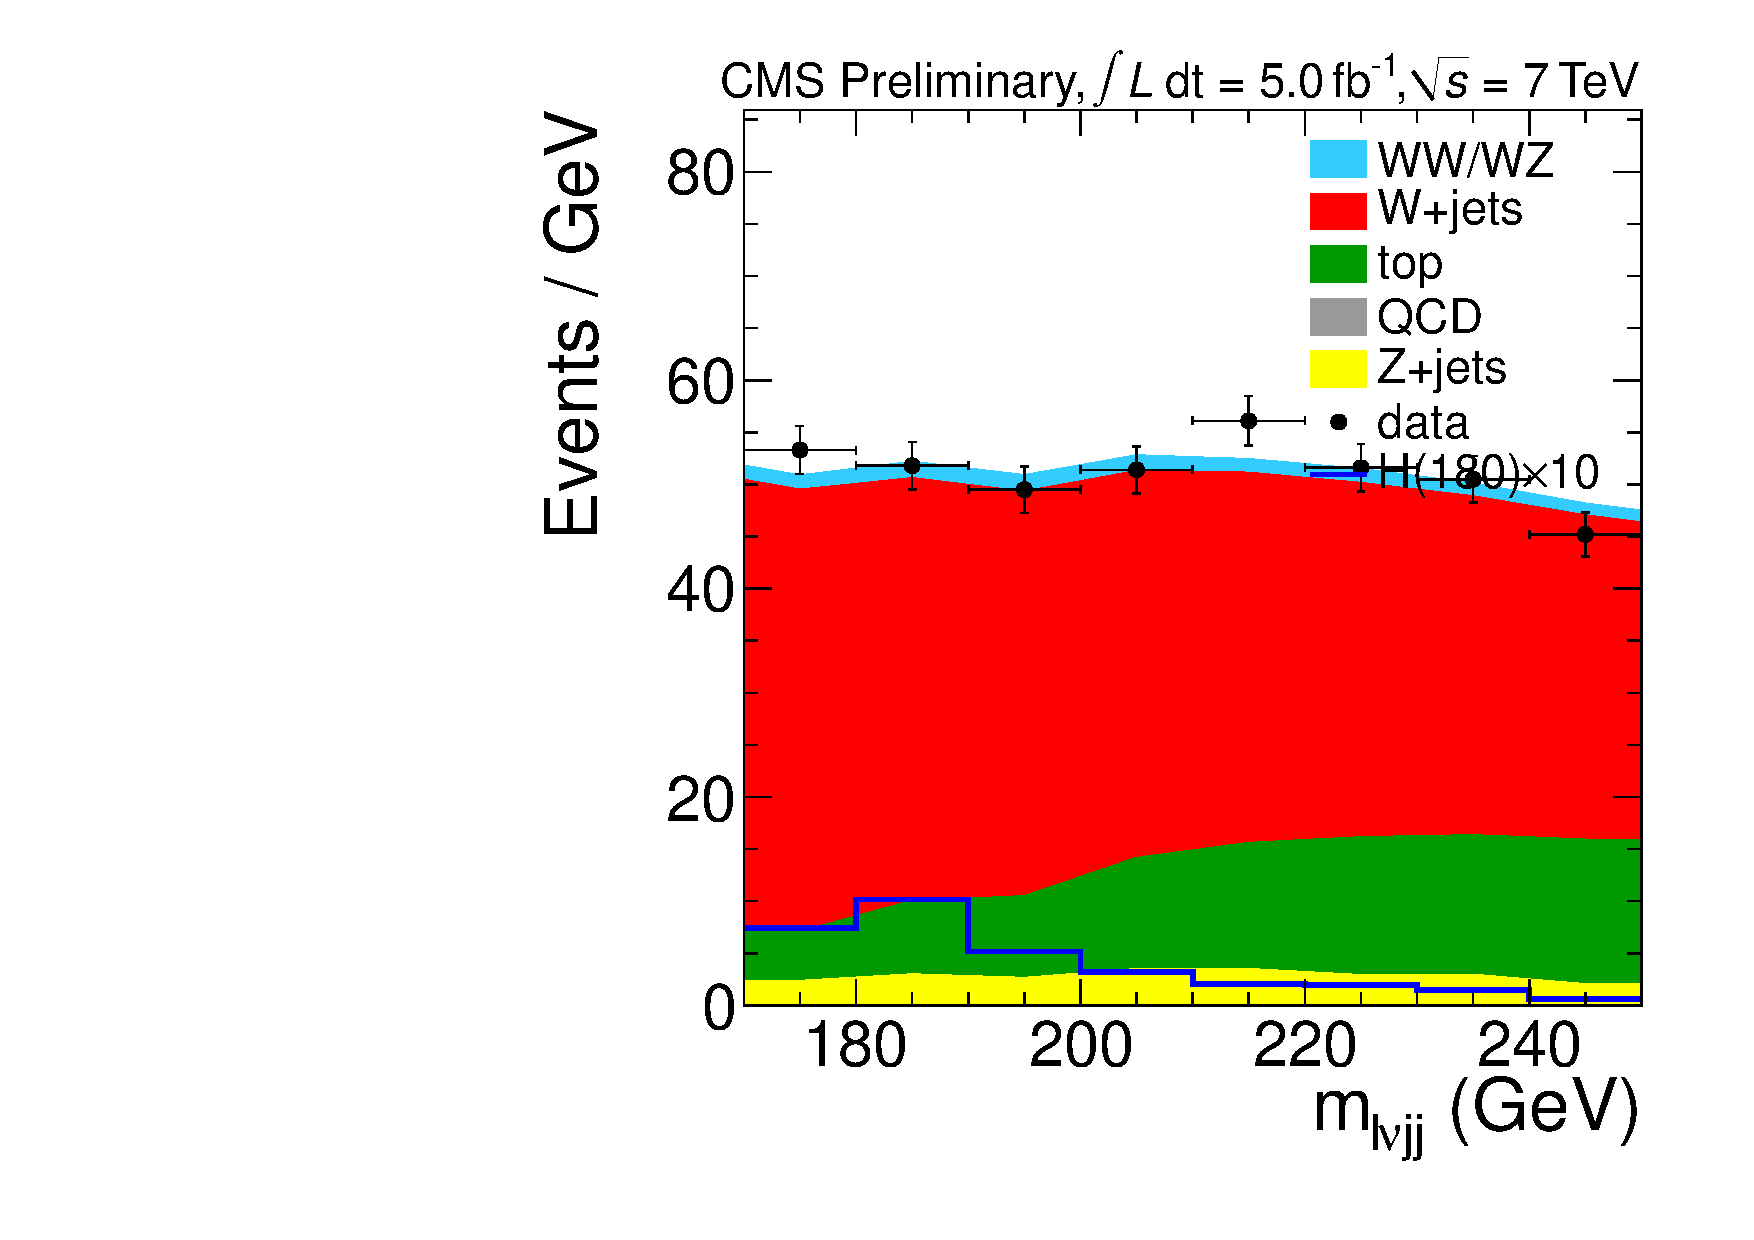
\includegraphics[width=0.3\textwidth]{plots/2012_FOURBSHAPES/H180_Mlvjj_Muon_3jets_Stacked}
%  }
%  \subfigure[]{
%    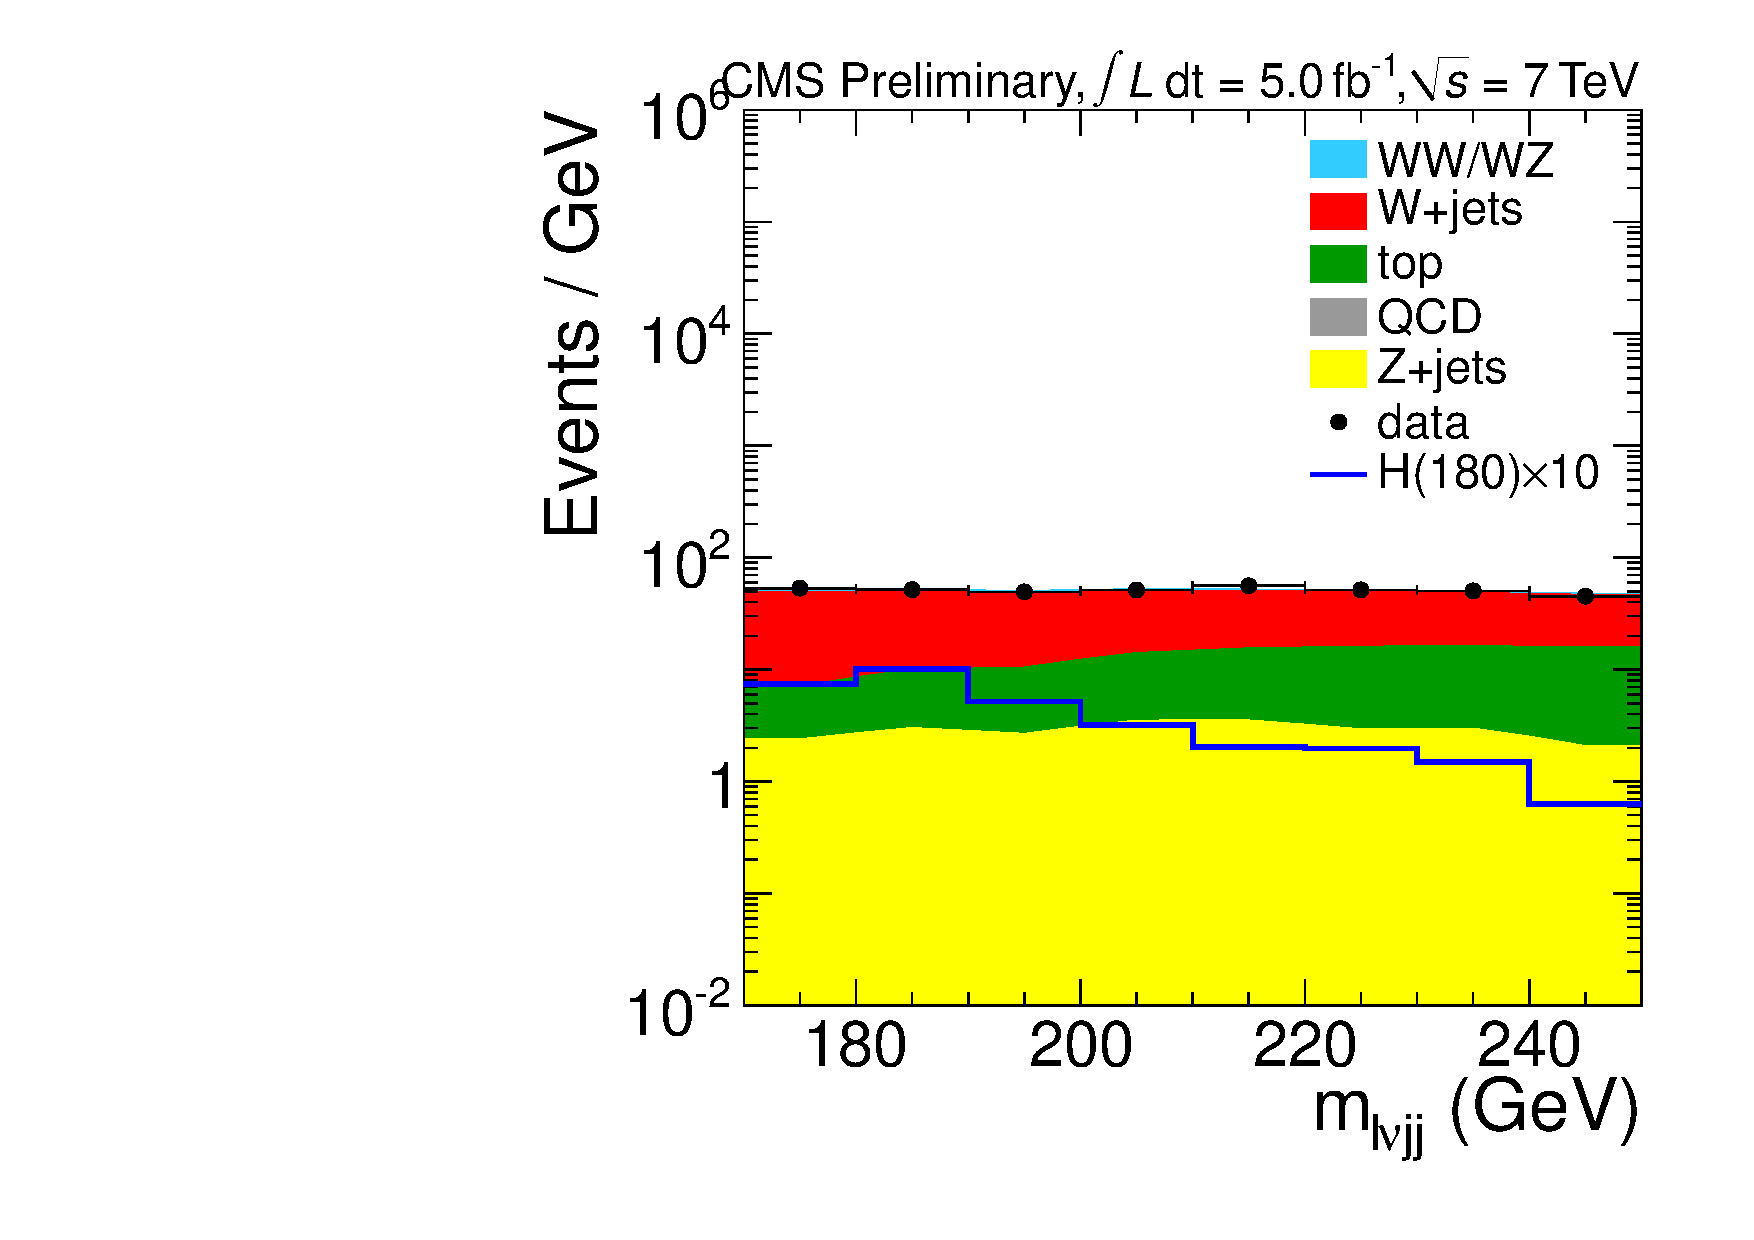
\includegraphics[width=0.3\textwidth]{plots/2012_FOURBSHAPES/H180_Mlvjj_Muon_3jets_Stacked_log}
%  }
%  \subfigure[]{
%    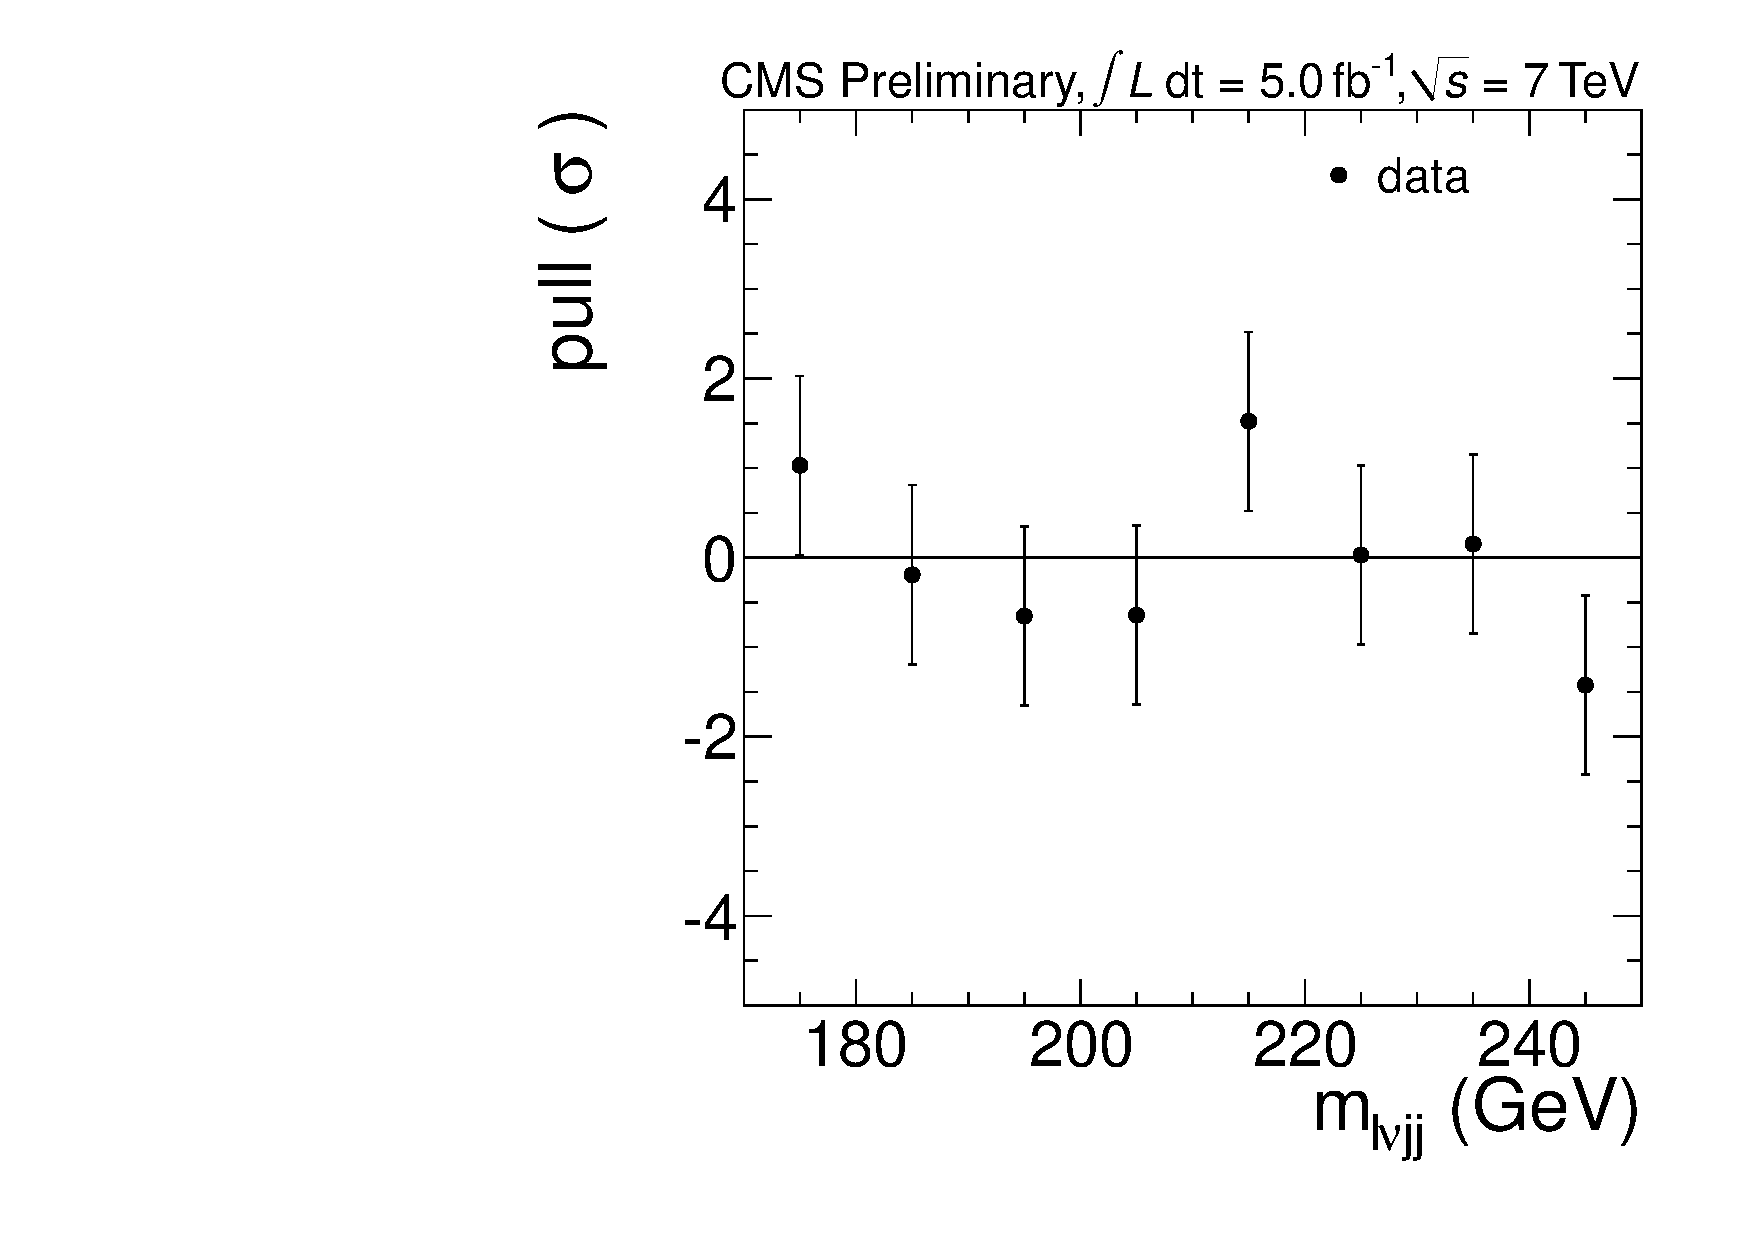
\includegraphics[width=0.3\textwidth]{plots/2012_FOURBSHAPES/H180_Mlvjj_Muon_3jets_Pull}
%  }
%  \vspace*{1mm} \\
%  \subfigure[]{
%      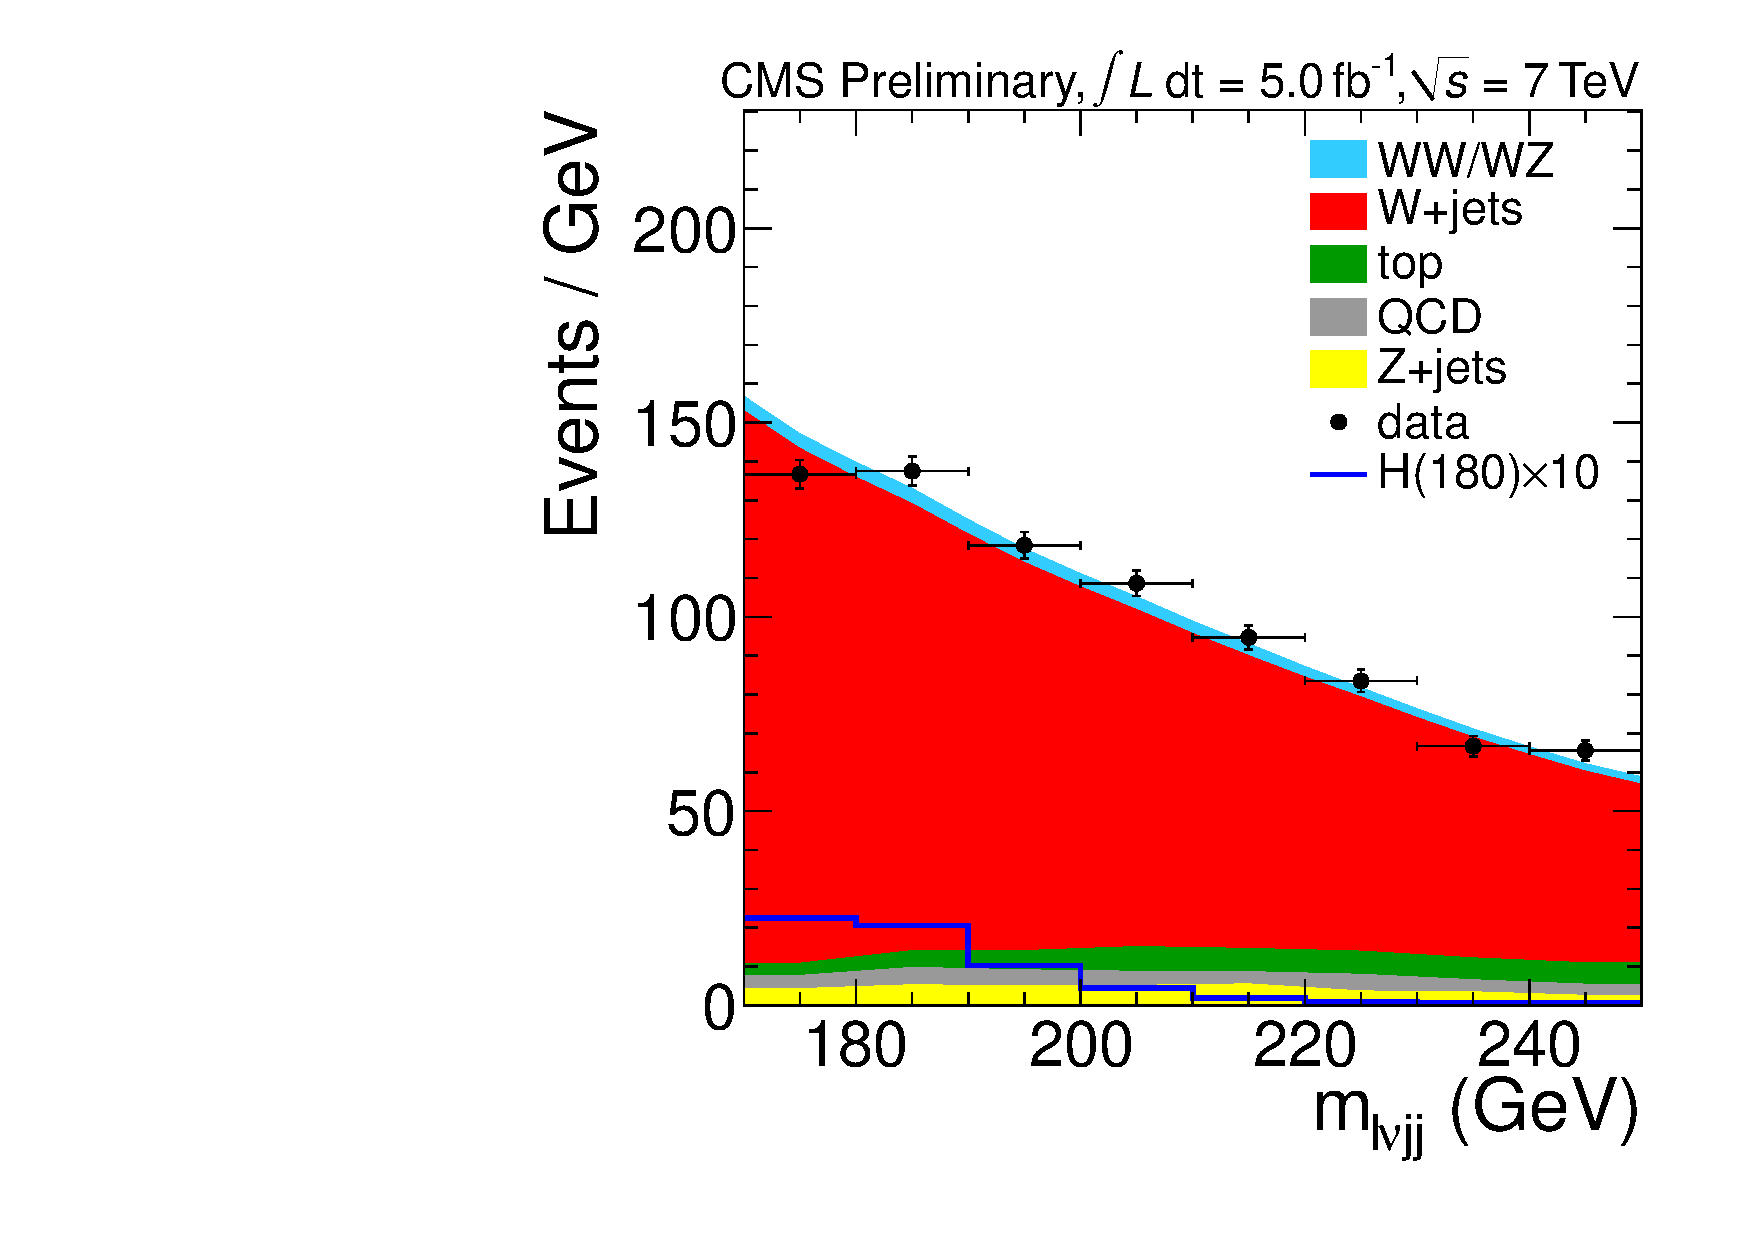
\includegraphics[width=0.3\textwidth]{plots/2012_FOURBSHAPES/H180_Mlvjj_Electron_2jets_Stacked}
%  }
%  \subfigure[]{
%    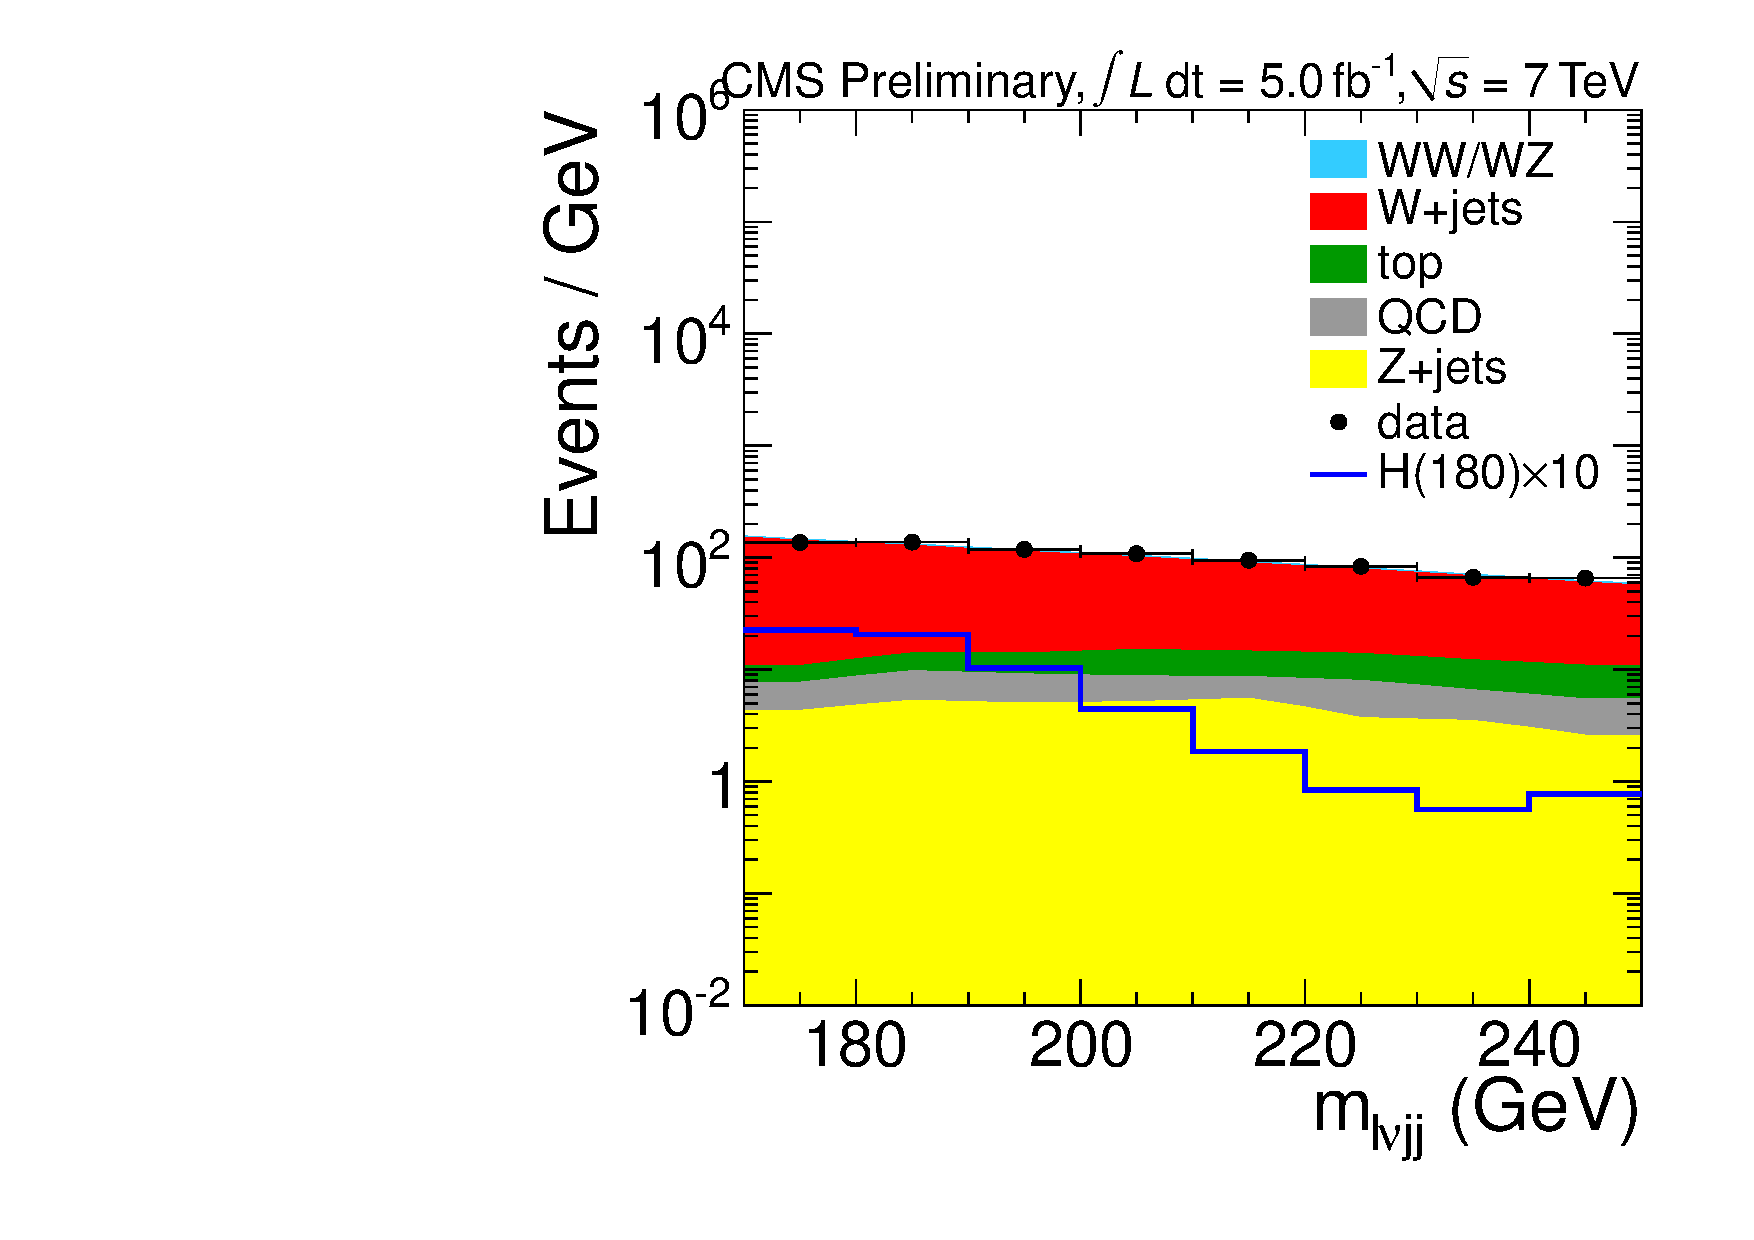
\includegraphics[width=0.3\textwidth]{plots/2012_FOURBSHAPES/H180_Mlvjj_Electron_2jets_Stacked_log}
%  }
%  \subfigure[]{
%    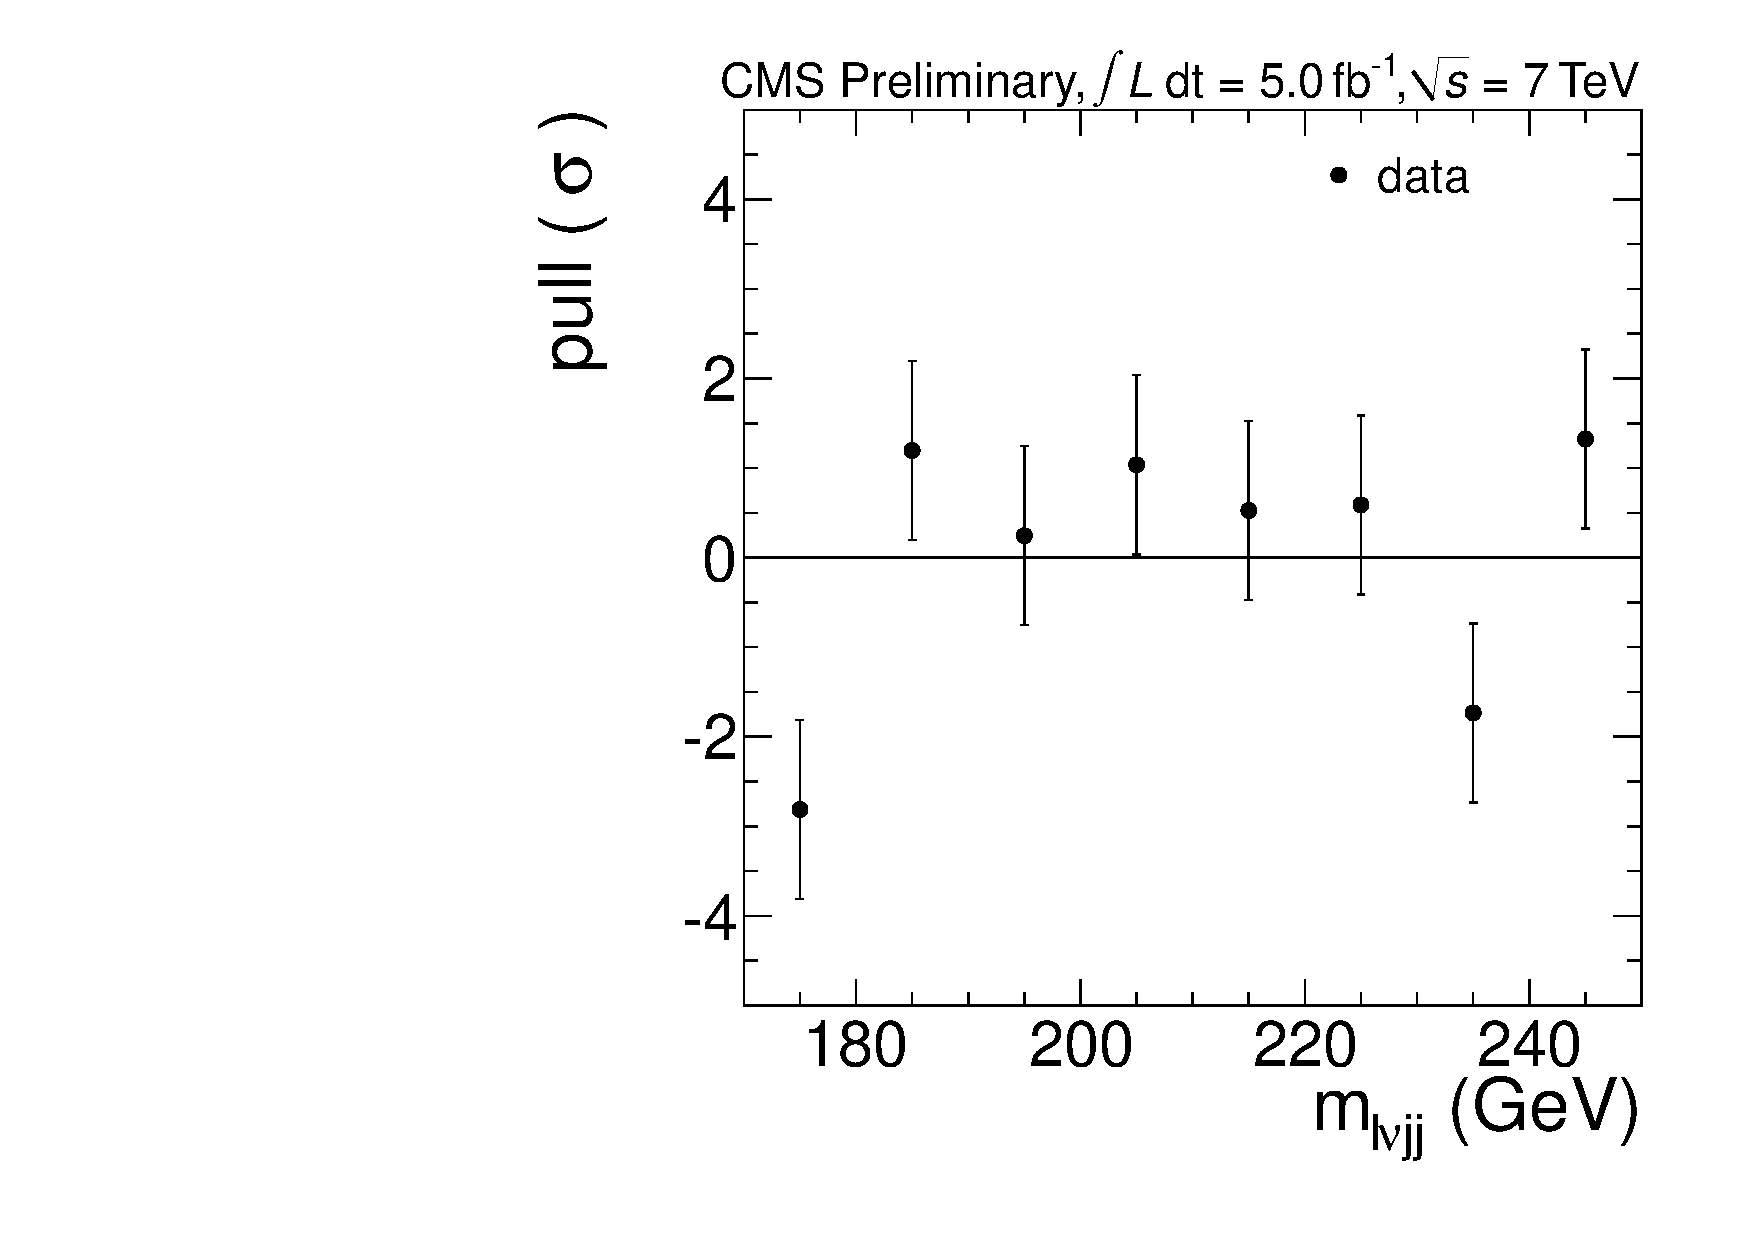
\includegraphics[width=0.3\textwidth]{plots/2012_FOURBSHAPES/H180_Mlvjj_Electron_2jets_Pull}
%  }
%  \vspace*{1mm} \\
%  \subfigure[]{
%      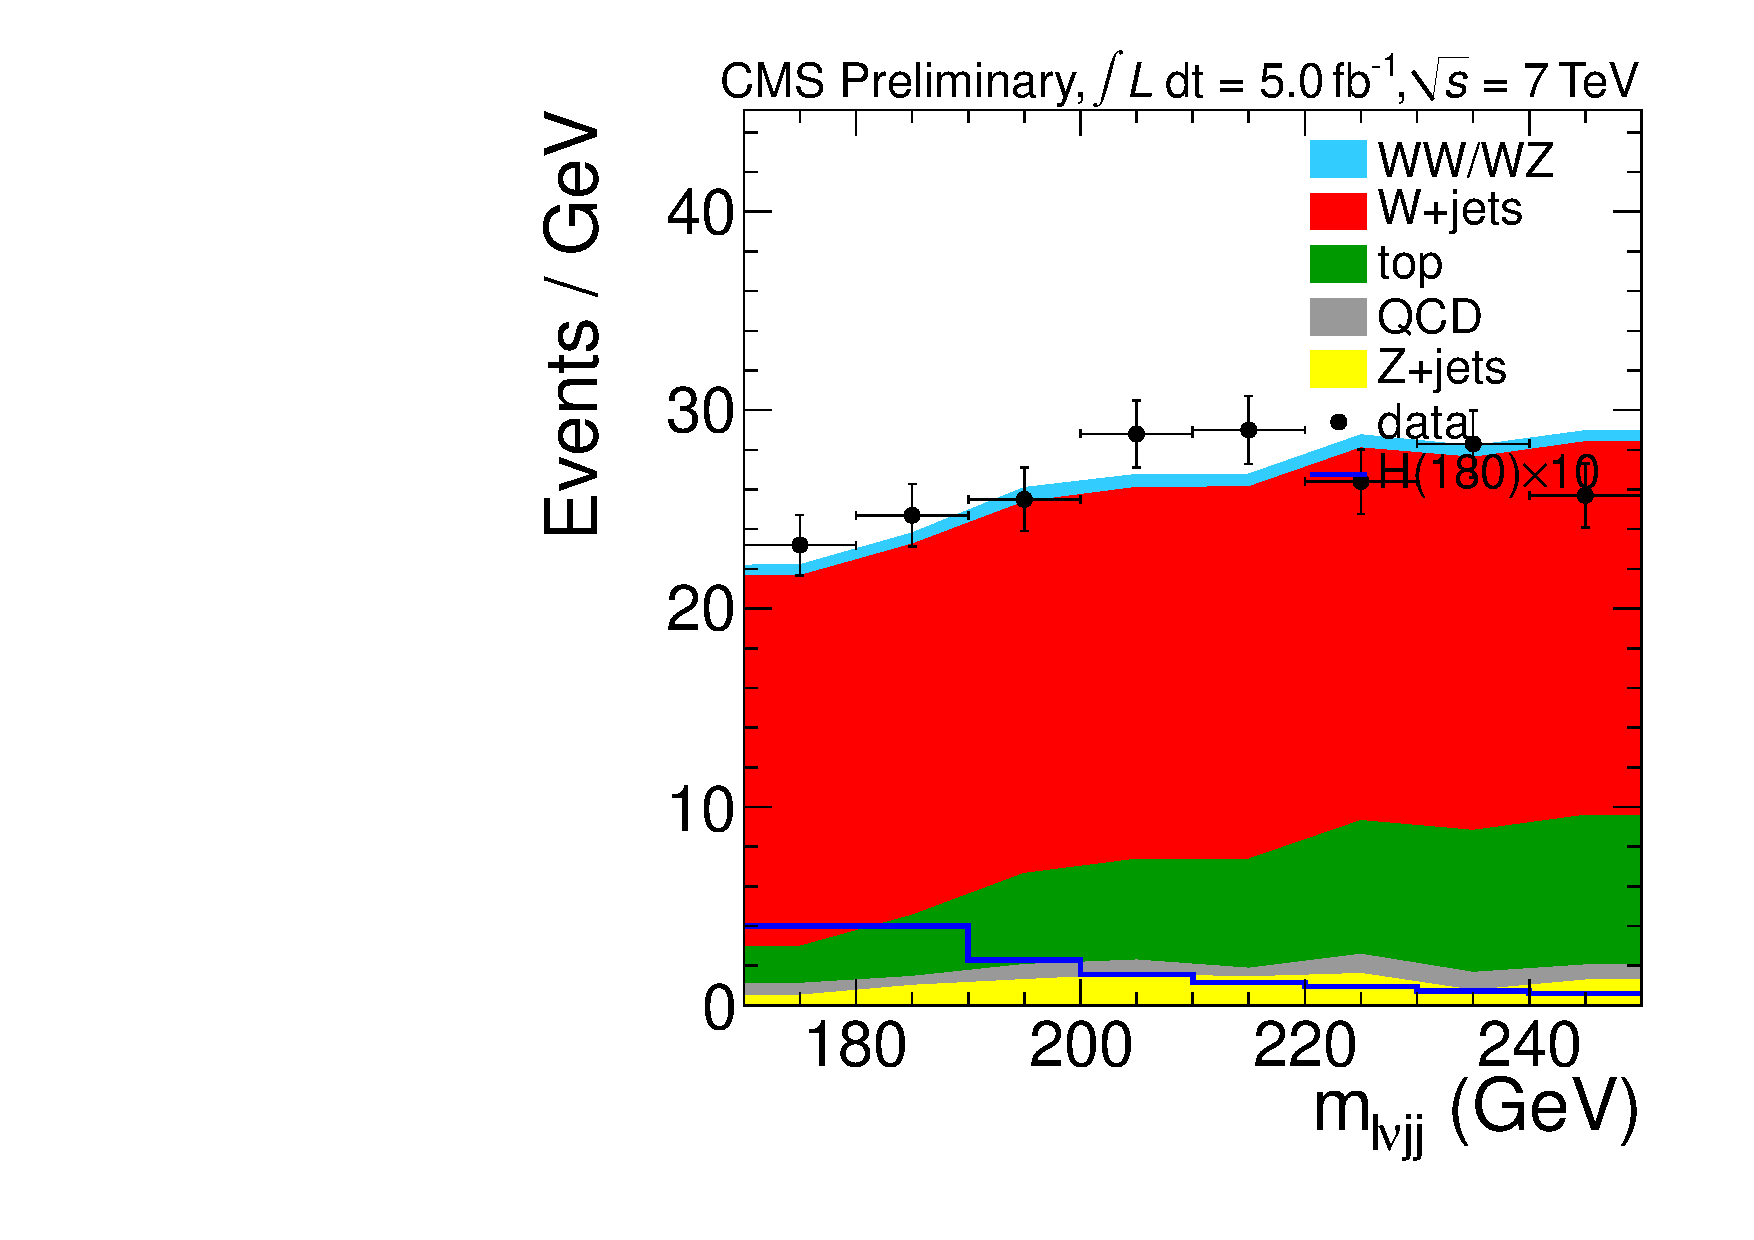
\includegraphics[width=0.3\textwidth]{plots/2012_FOURBSHAPES/H180_Mlvjj_Electron_3jets_Stacked}
%  }
%  \subfigure[]{
%    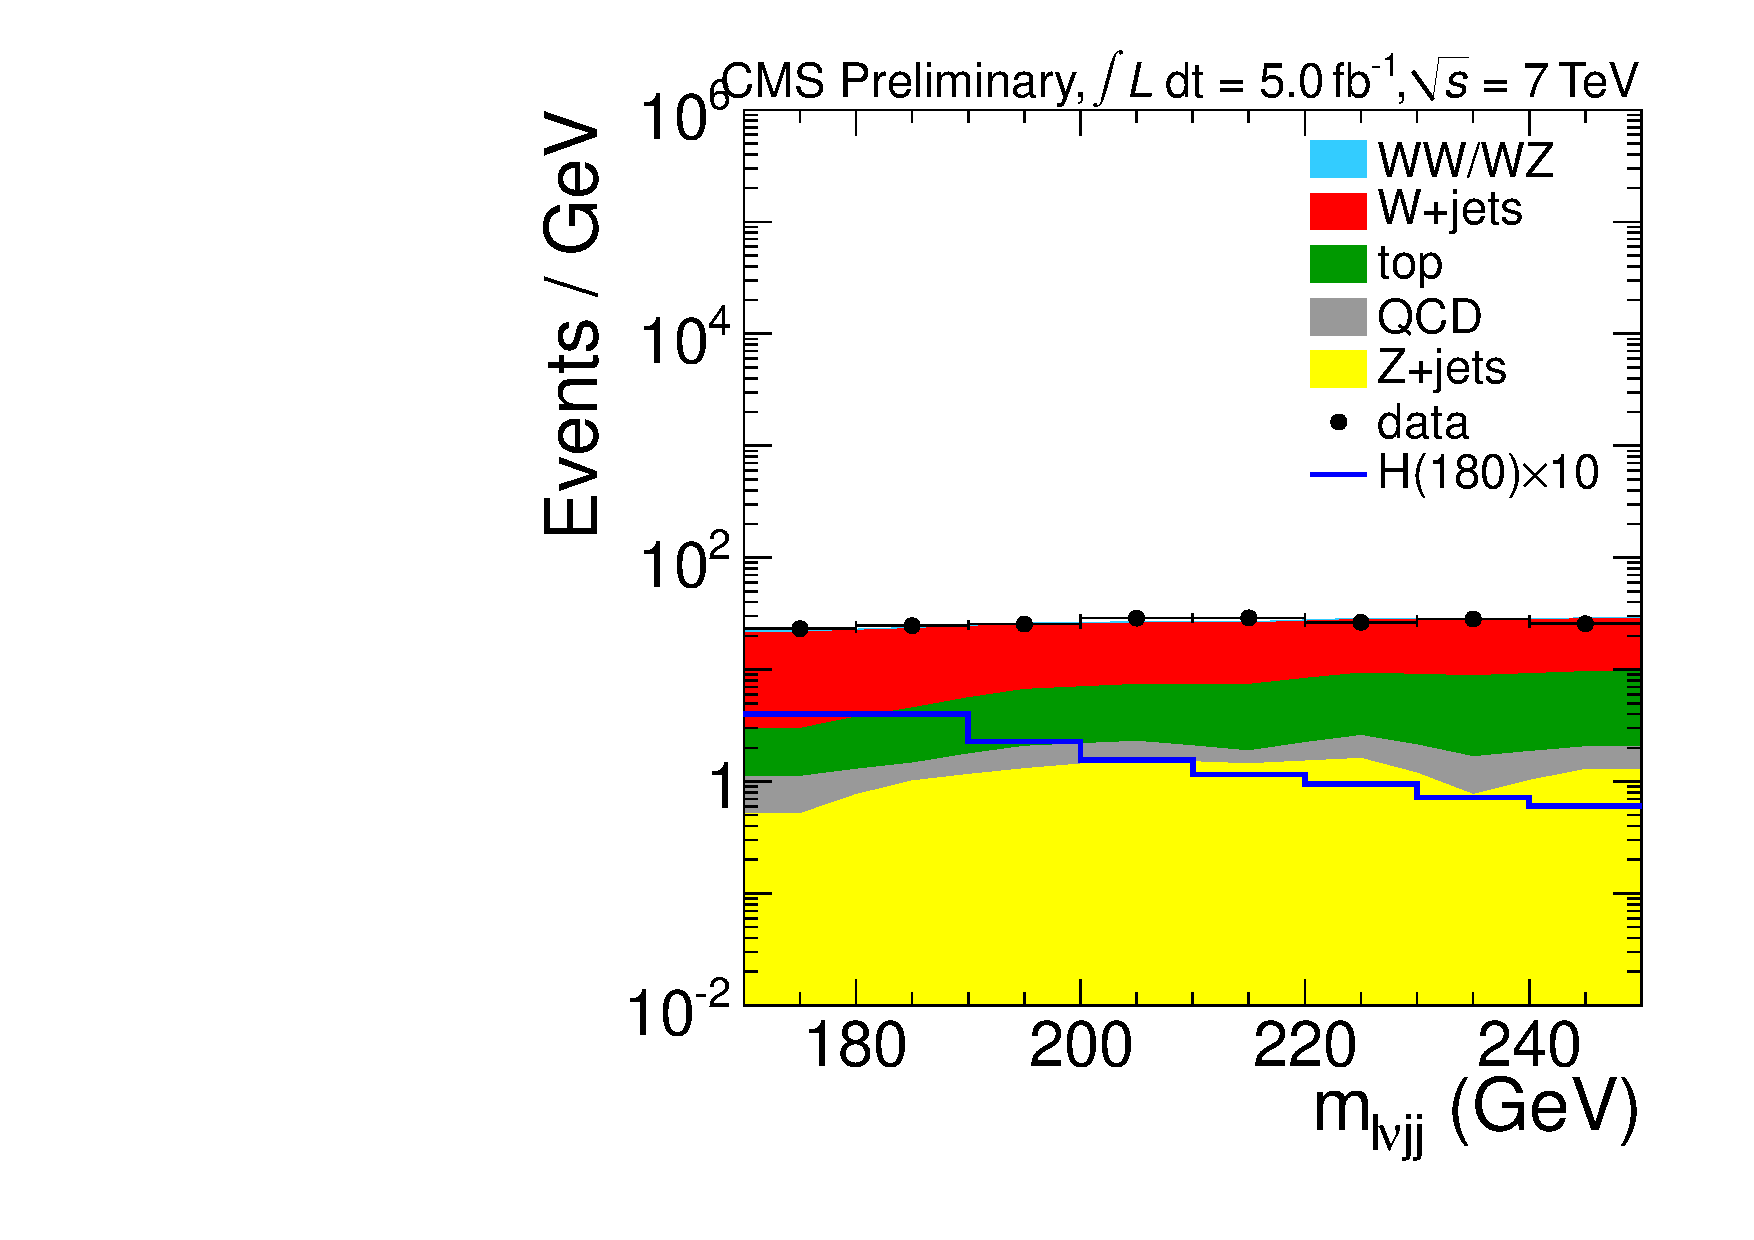
\includegraphics[width=0.3\textwidth]{plots/2012_FOURBSHAPES/H180_Mlvjj_Electron_3jets_Stacked_log}
%  }
%  \subfigure[]{
%    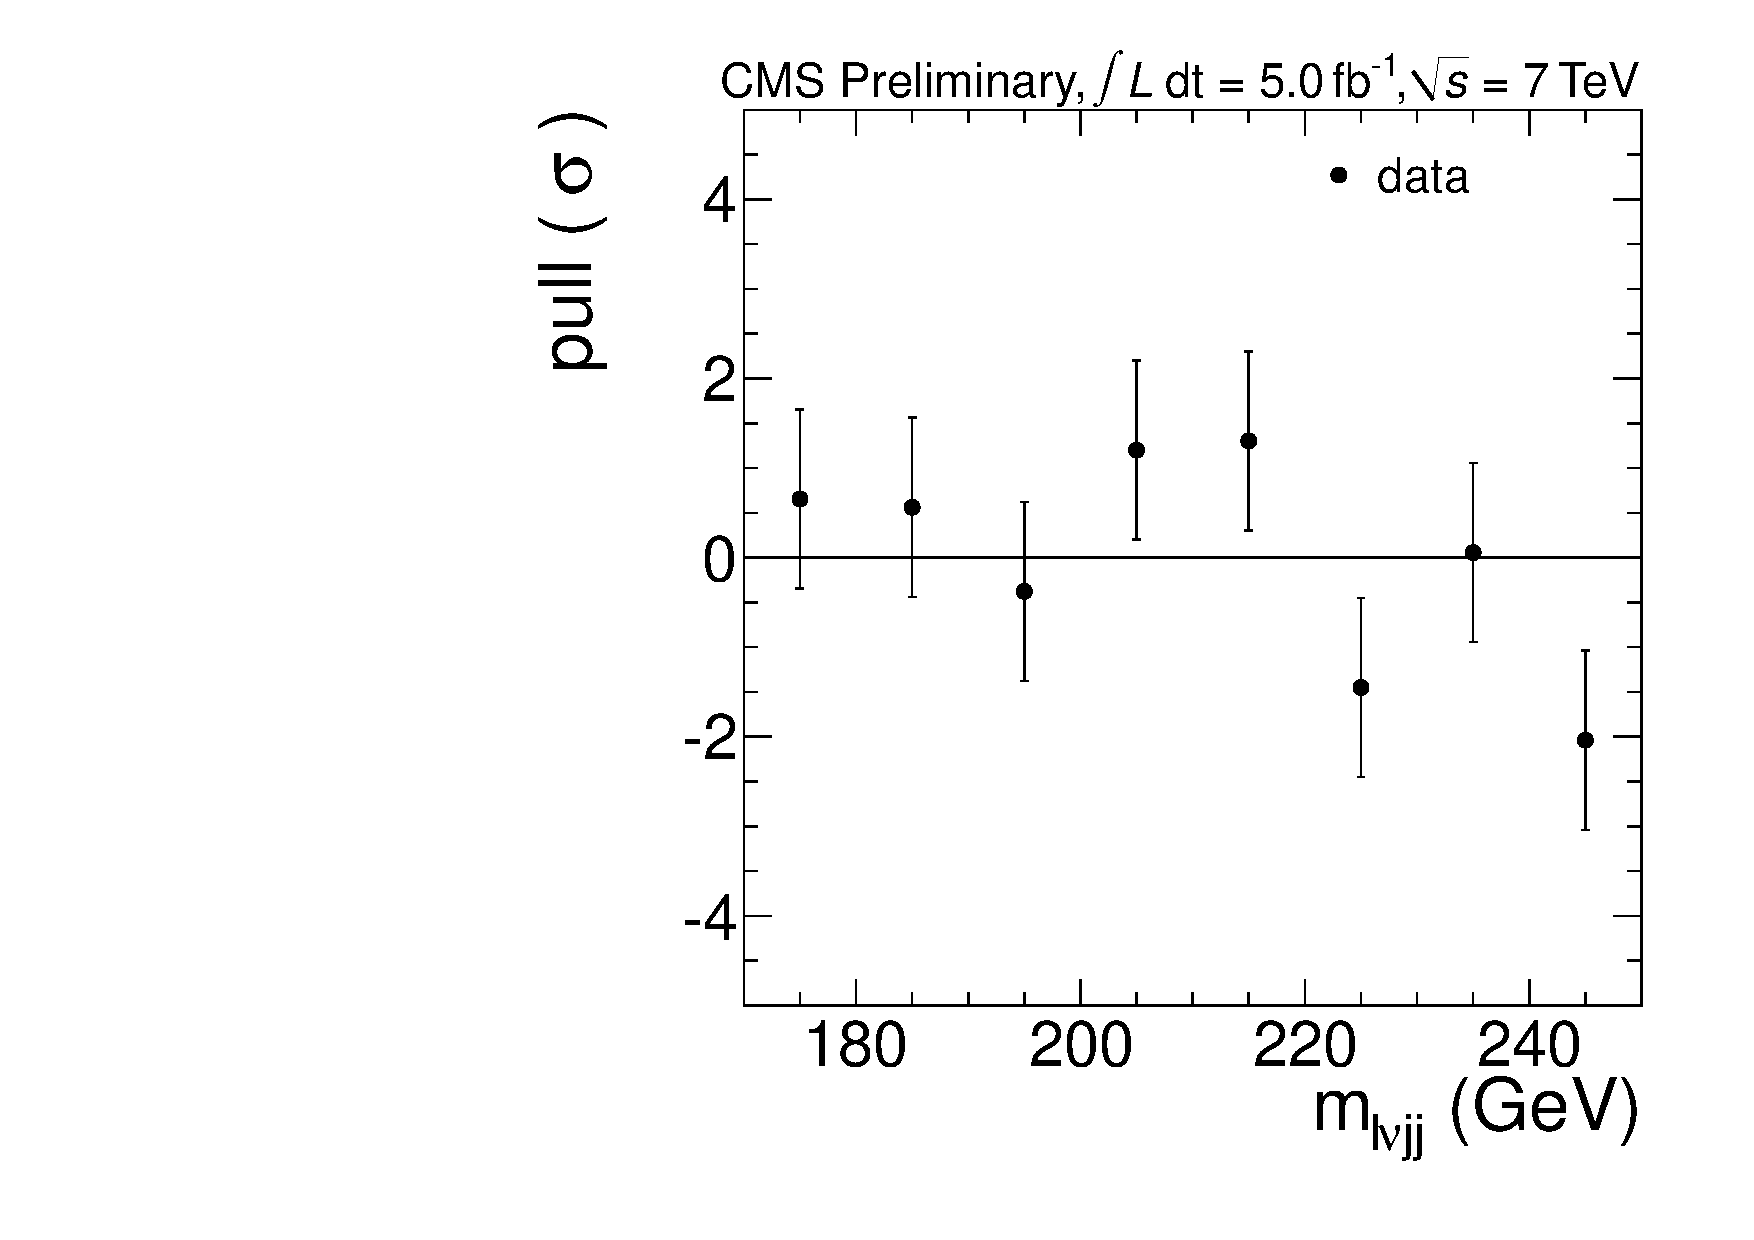
\includegraphics[width=0.3\textwidth]{plots/2012_FOURBSHAPES/H180_Mlvjj_Electron_3jets_Pull}
%  }
%  \caption{$M_H = 180$~GeV point. The distribution of the 4-body invariant mass $m_{\ell\nu jj}$ plotted on 
%  linear (left) and log (center) scales. The pull distribution computed as 
%  [(Data - Background)/ Background uncertainty] is shown on the right.
%  The four rows correspond to muon 2-jets, muon 3-jets, electron 2-jets, 
%  and electron 3-jets event categories, respectively. }
%  \label{fig:mlnujj_mH180}
%  \end{figure}
%%%%%%%%%%%%%%%%%%%%
%%%%%%%%%%%%%%%%%%%%
%%%%%%%%%%%%%%%%%%%%
%  \begin{figure}[h!t]
%  \subfigure[]{
%      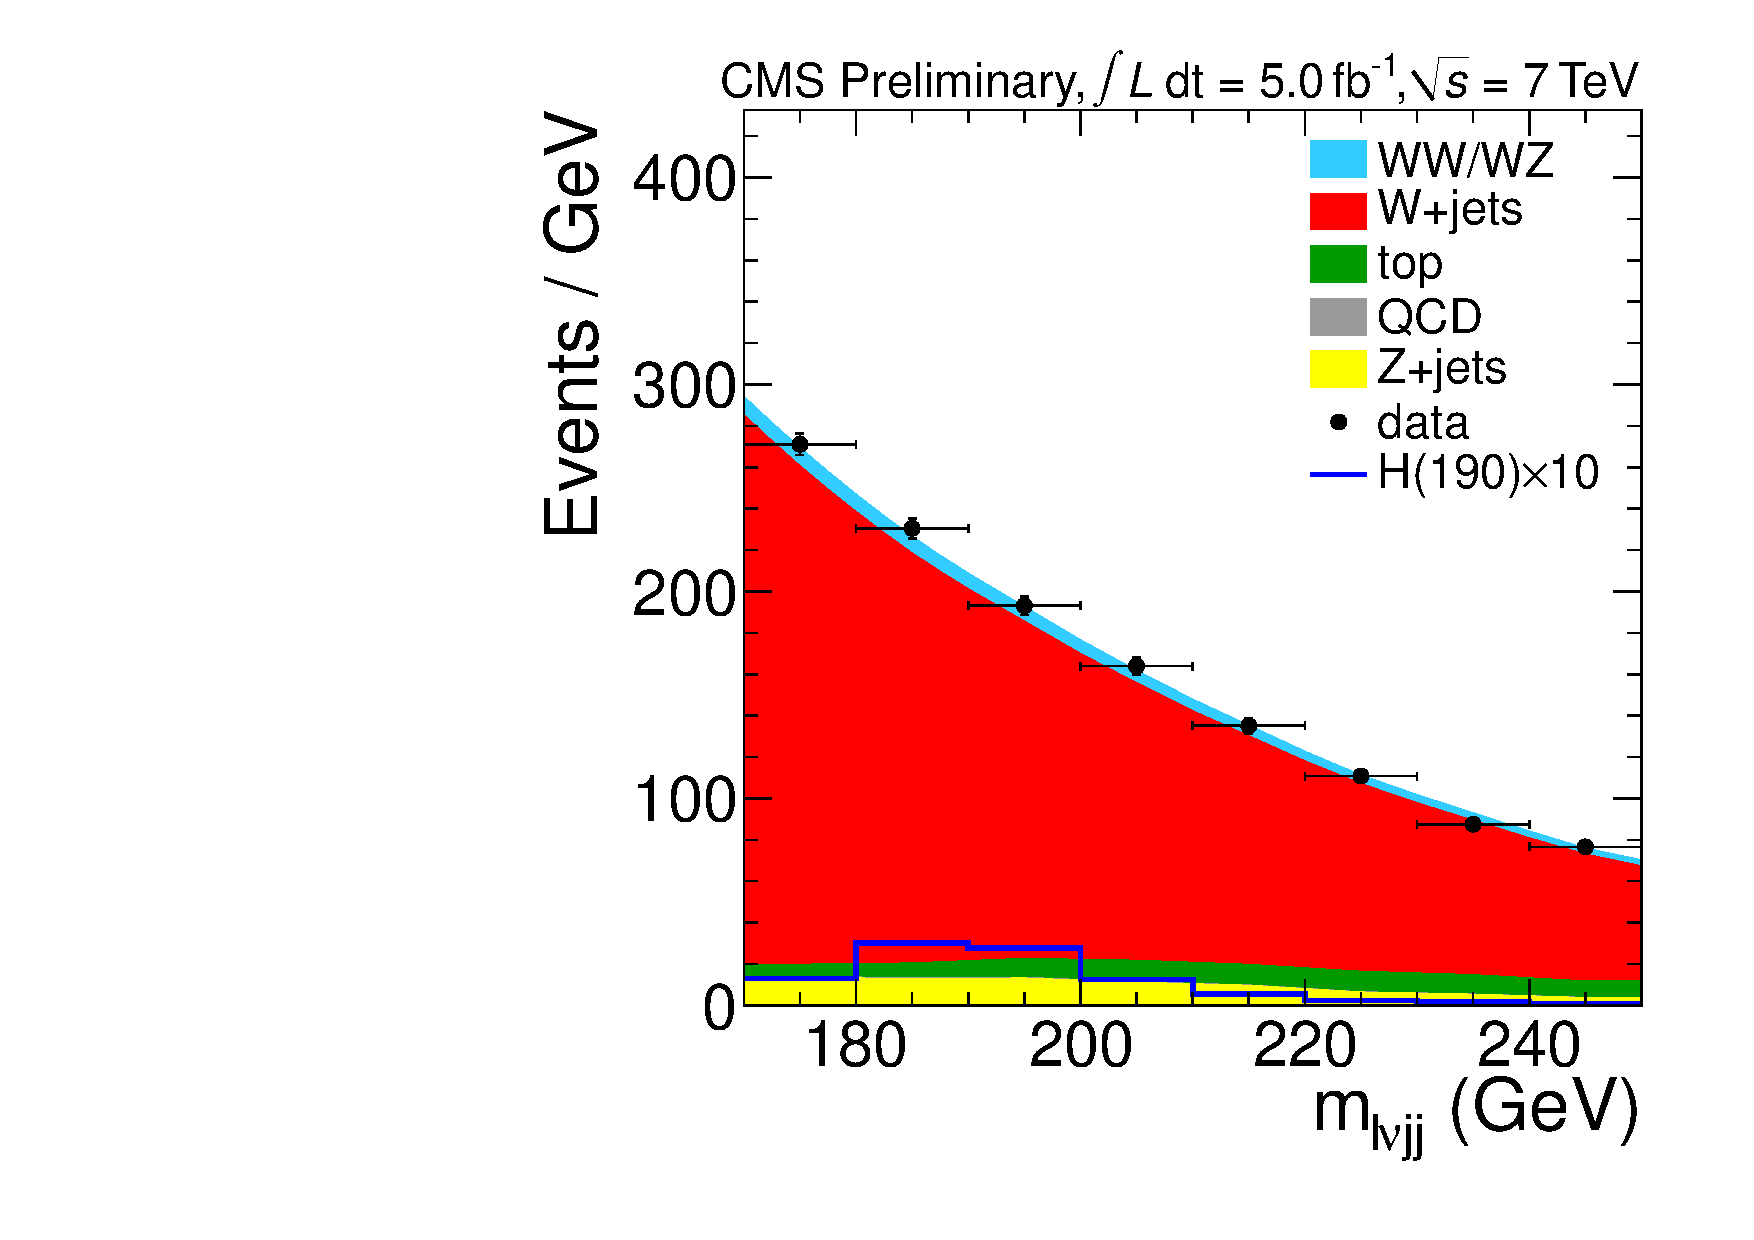
\includegraphics[width=0.3\textwidth]{plots/2012_FOURBSHAPES/H190_Mlvjj_Muon_2jets_Stacked}
%  }
%  \subfigure[]{
%    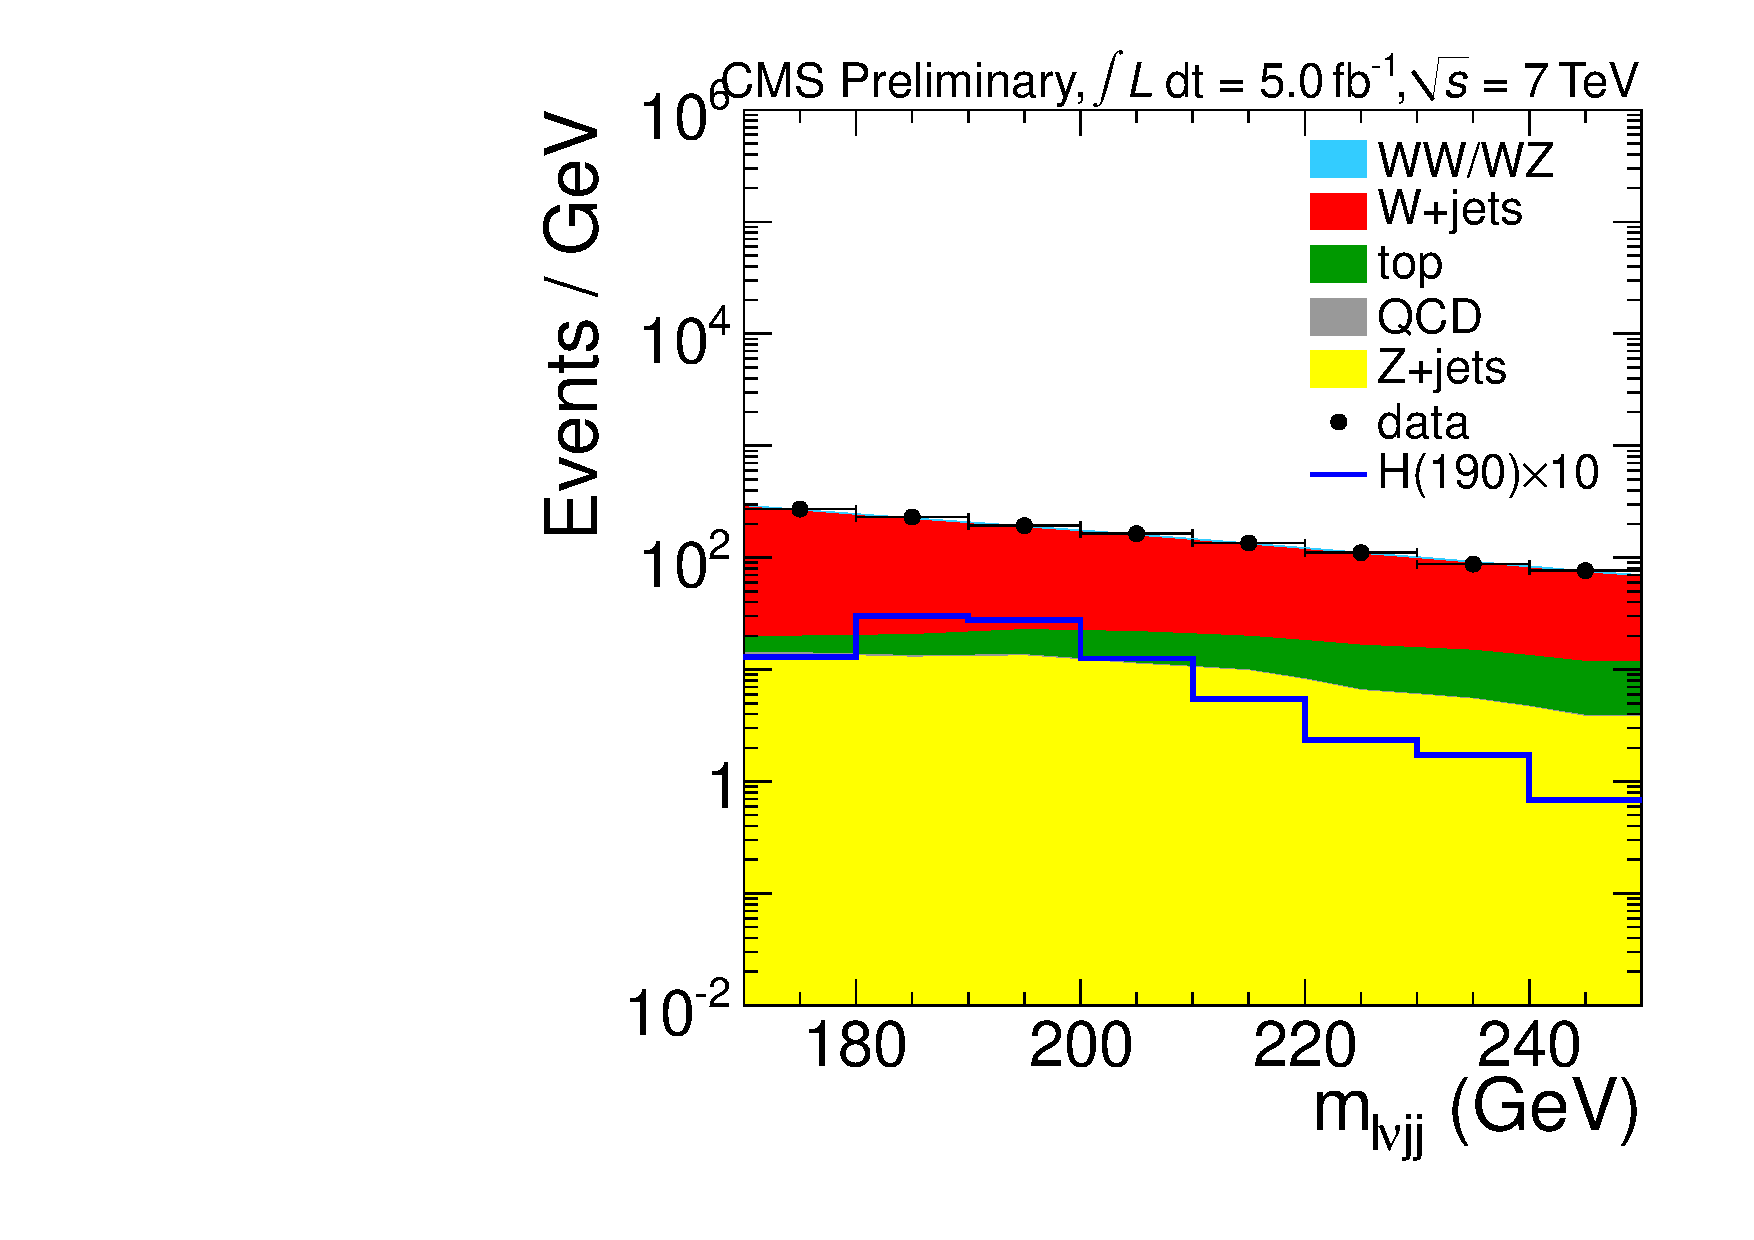
\includegraphics[width=0.3\textwidth]{plots/2012_FOURBSHAPES/H190_Mlvjj_Muon_2jets_Stacked_log}
%  }
%  \subfigure[]{
%    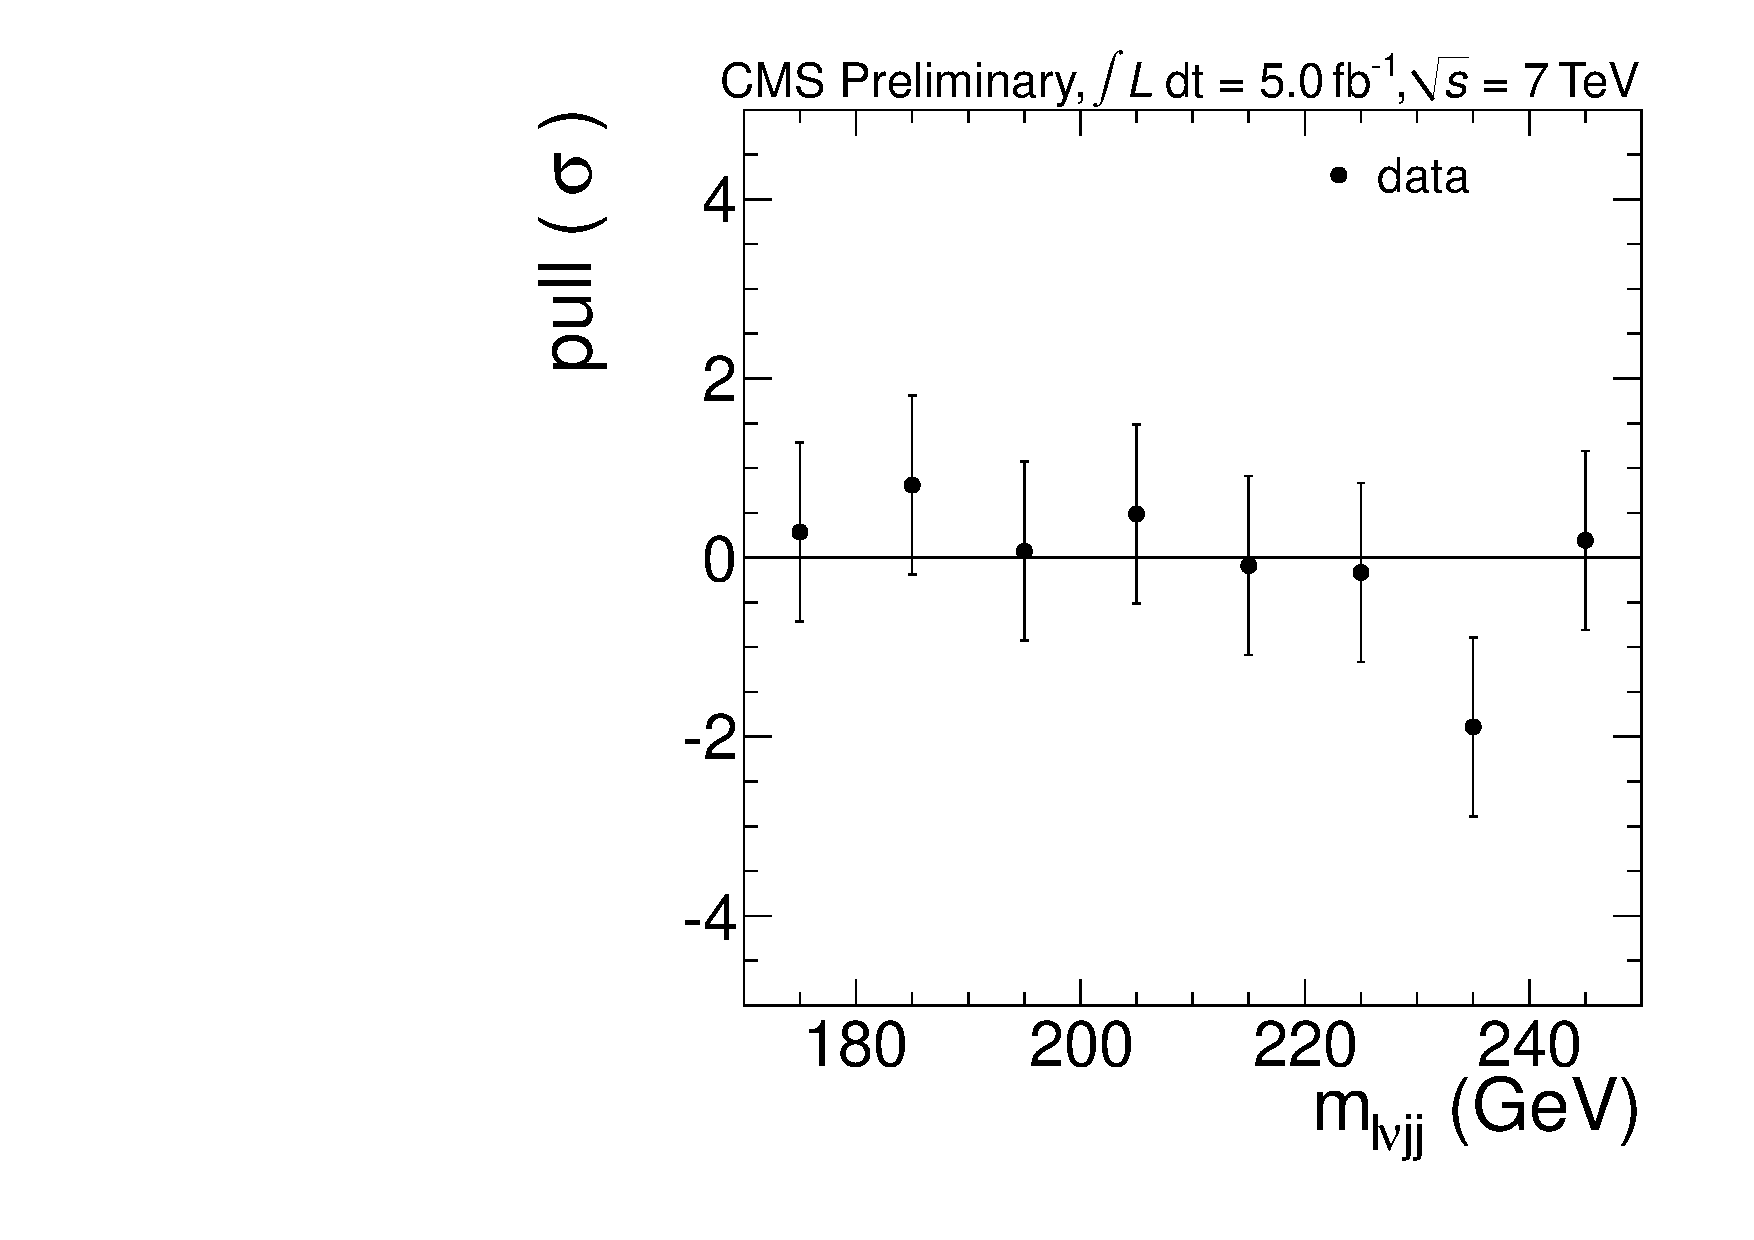
\includegraphics[width=0.3\textwidth]{plots/2012_FOURBSHAPES/H190_Mlvjj_Muon_2jets_Pull}
%  }
%  \vspace*{1mm} \\
%  \subfigure[]{
%      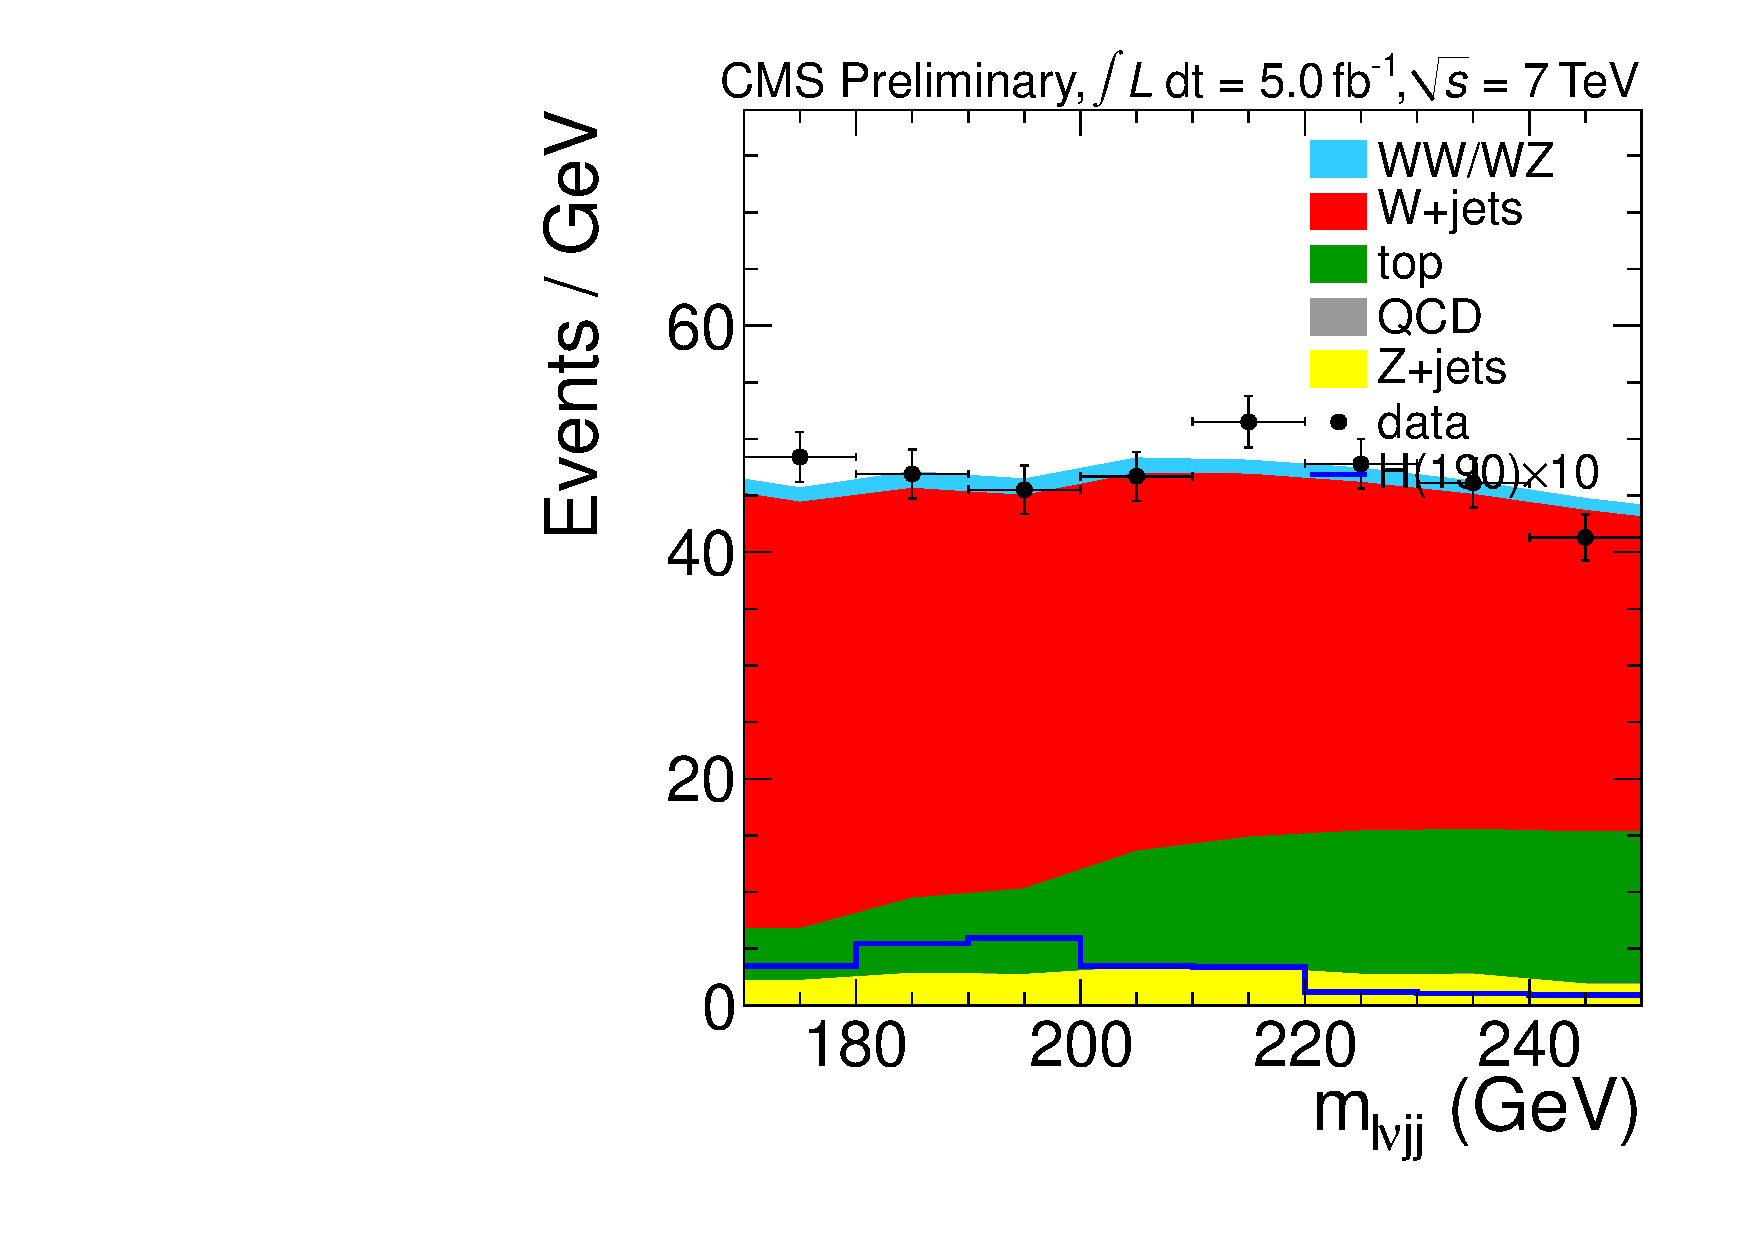
\includegraphics[width=0.3\textwidth]{plots/2012_FOURBSHAPES/H190_Mlvjj_Muon_3jets_Stacked}
%  }
%  \subfigure[]{
%    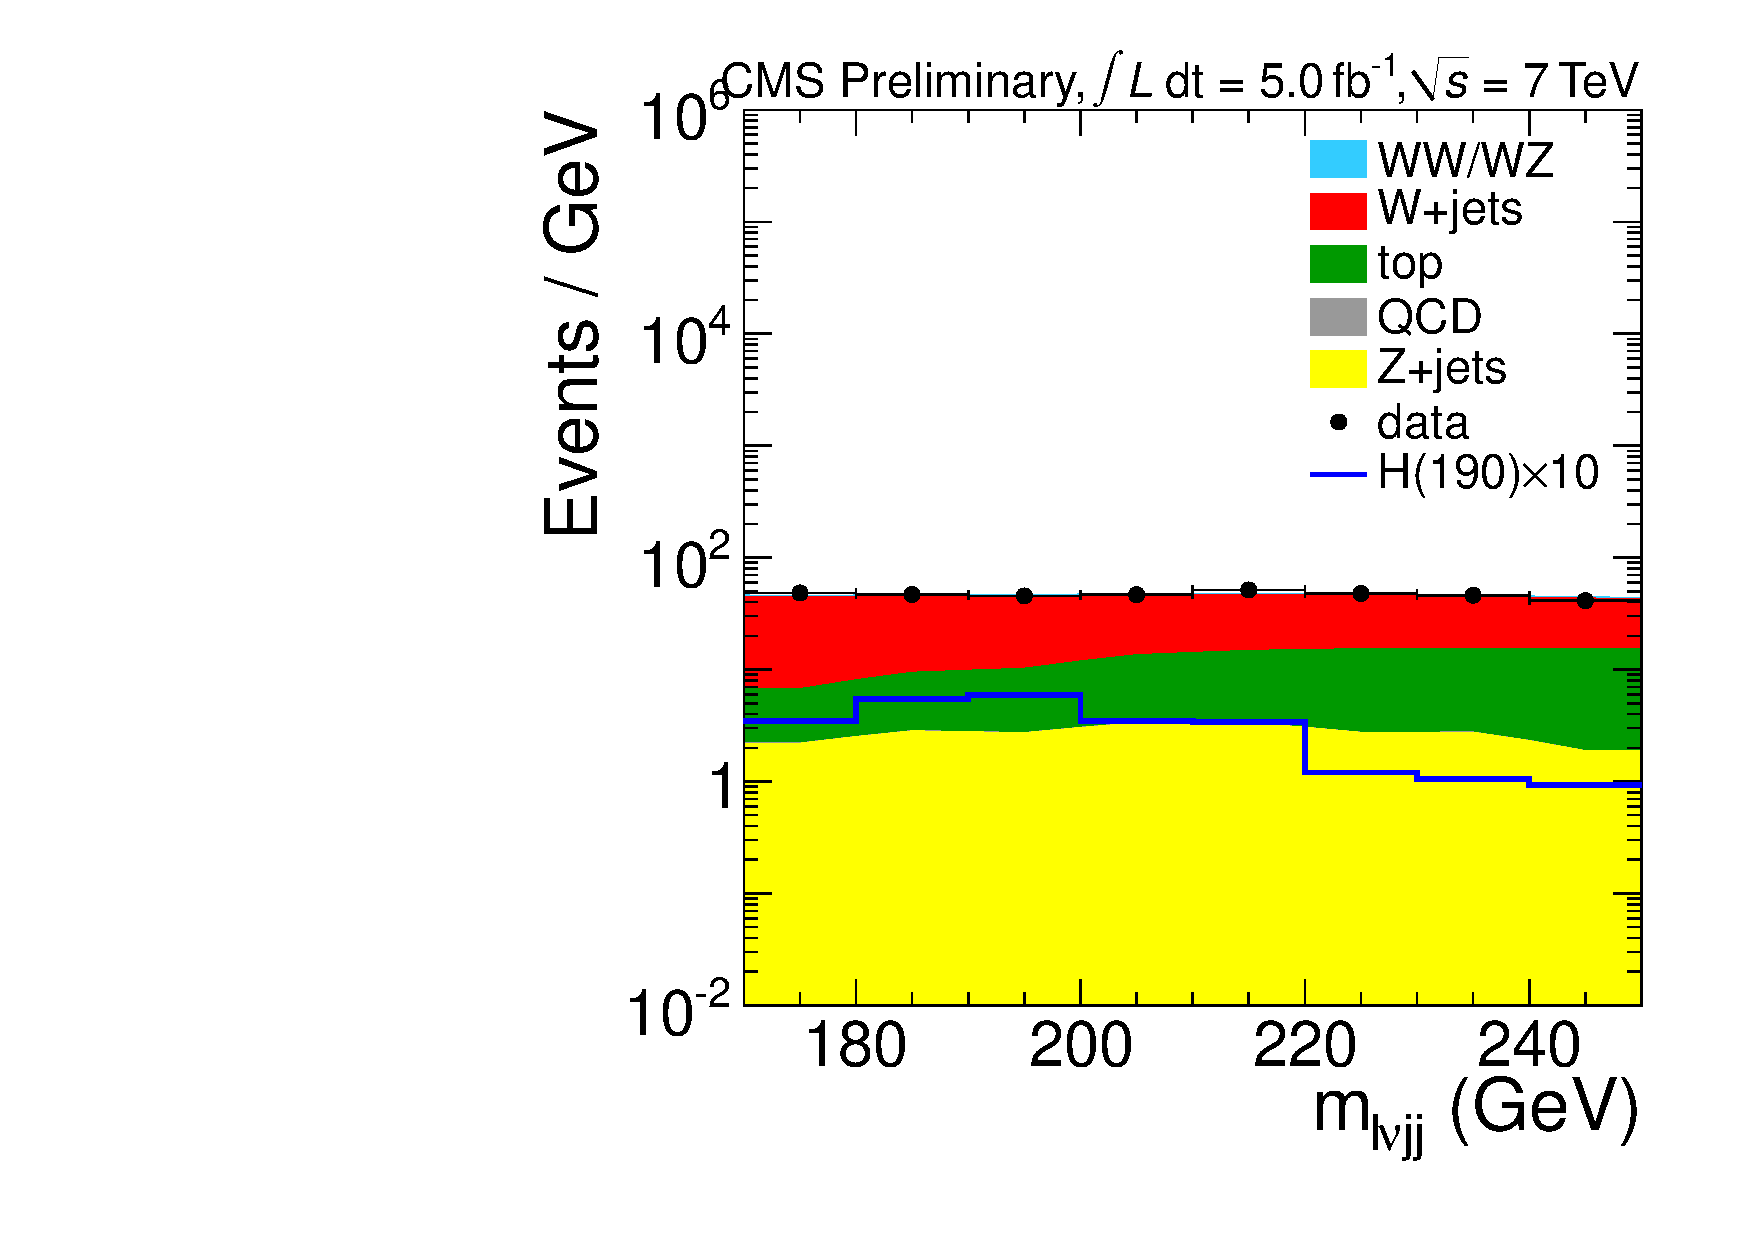
\includegraphics[width=0.3\textwidth]{plots/2012_FOURBSHAPES/H190_Mlvjj_Muon_3jets_Stacked_log}
%  }
%  \subfigure[]{
%    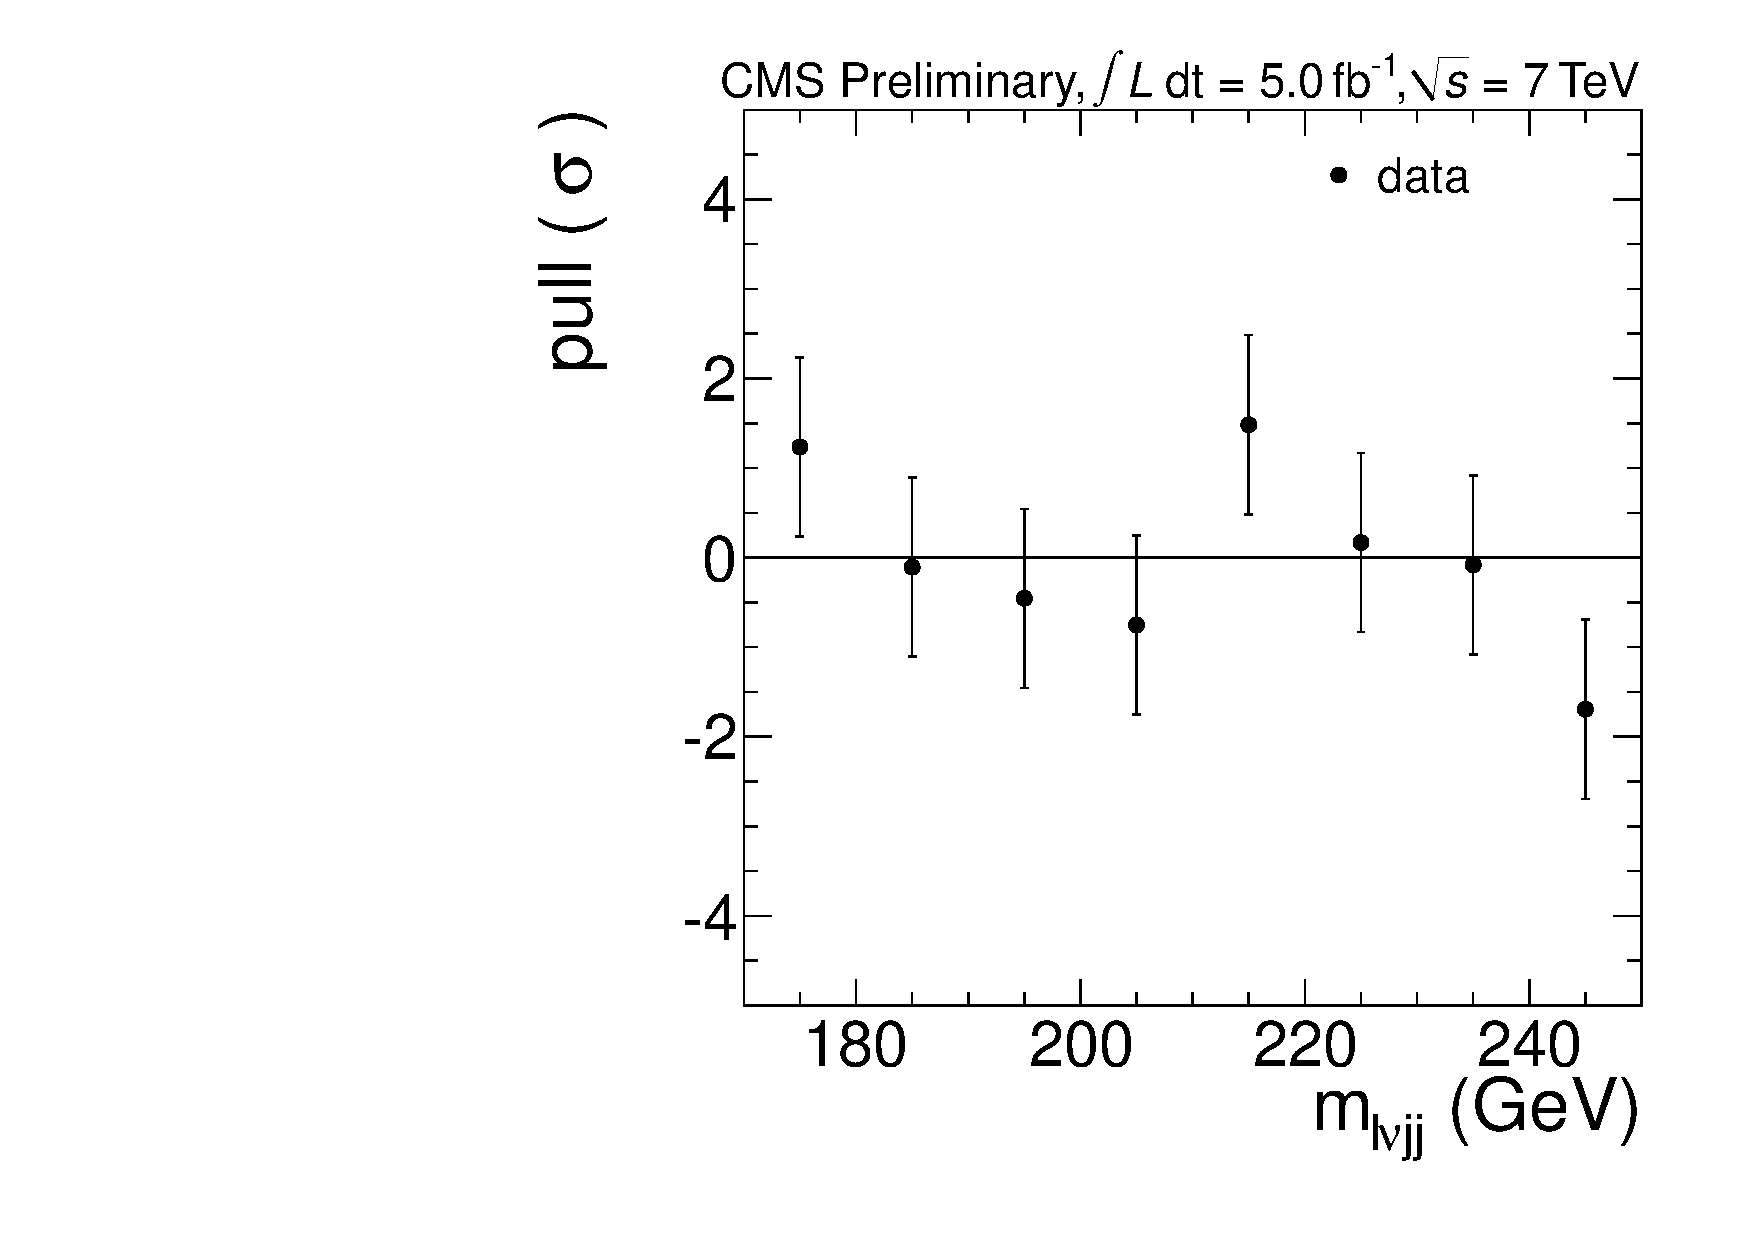
\includegraphics[width=0.3\textwidth]{plots/2012_FOURBSHAPES/H190_Mlvjj_Muon_3jets_Pull}
%  }
%  \vspace*{1mm} \\
%  \subfigure[]{
%      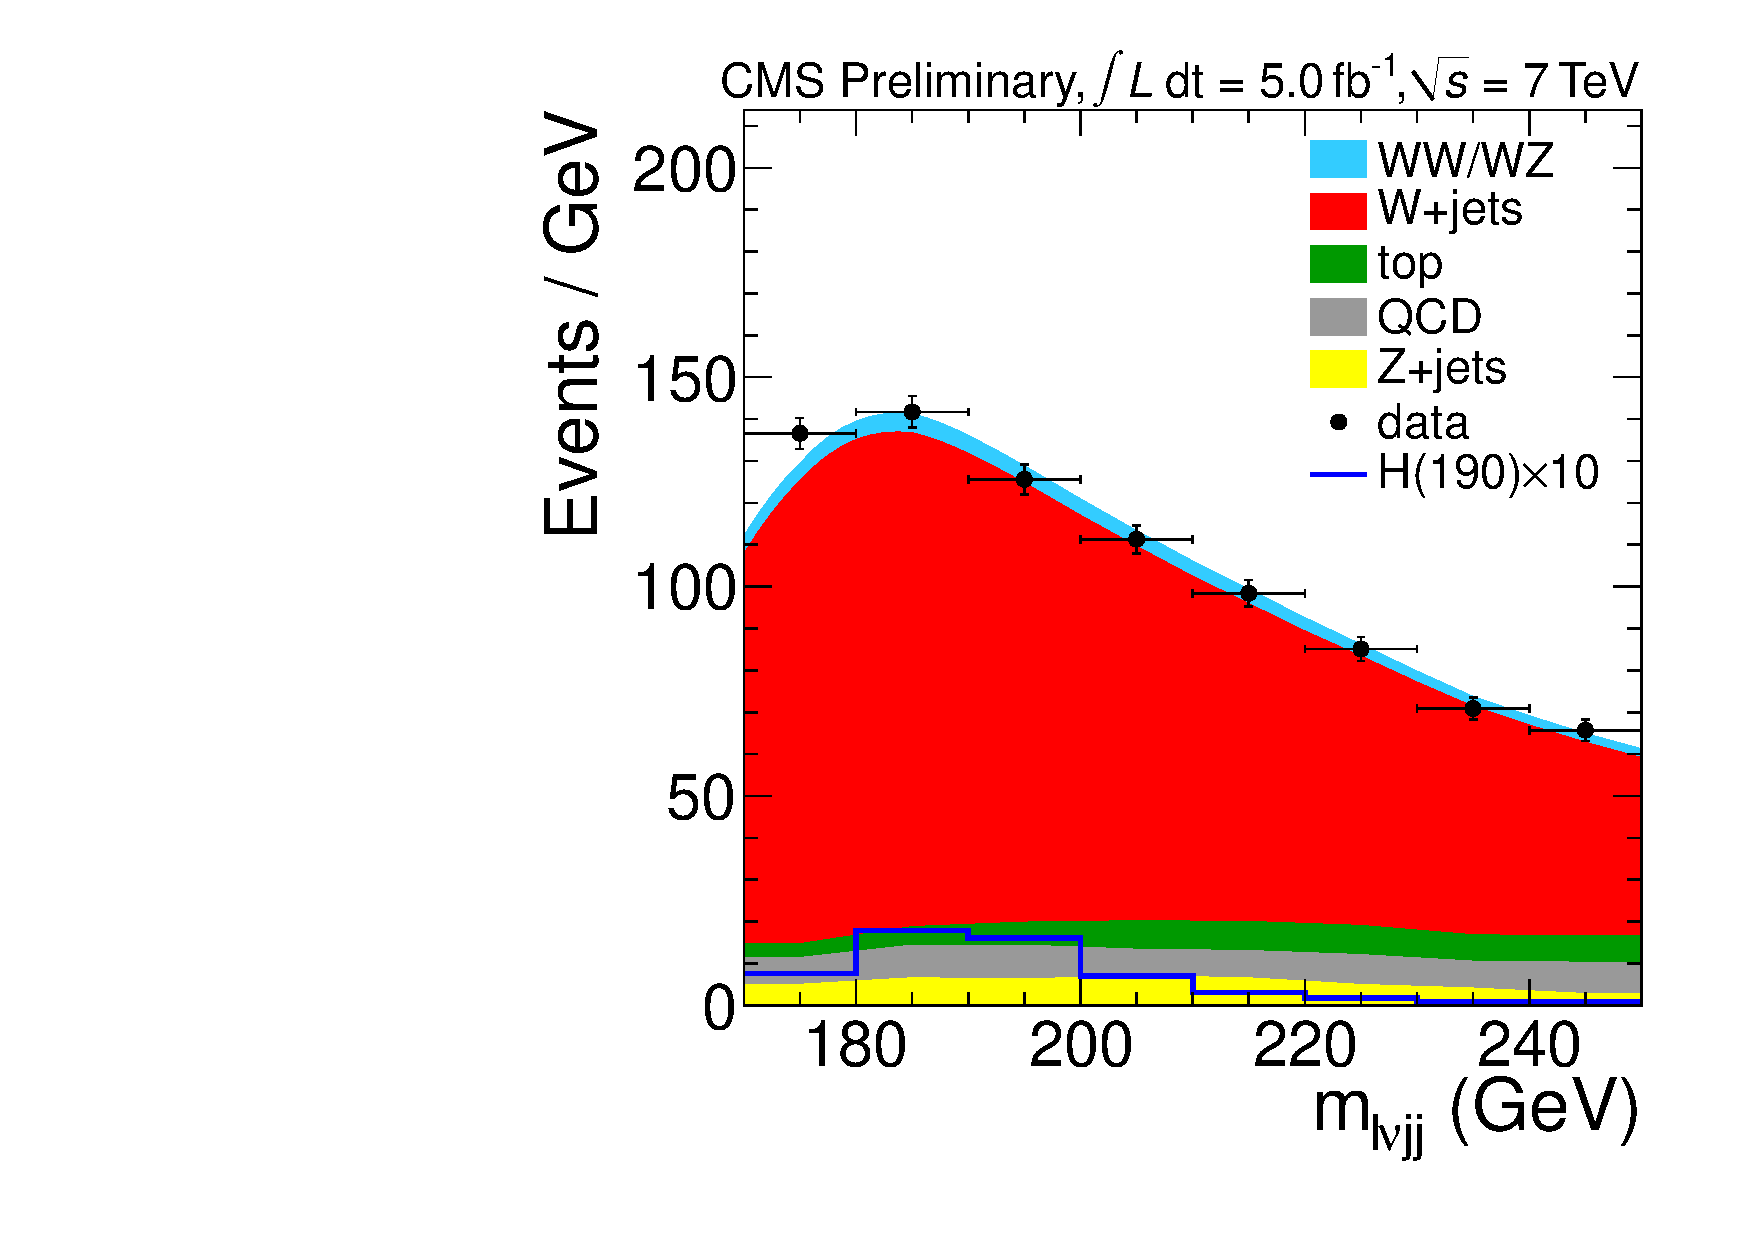
\includegraphics[width=0.3\textwidth]{plots/2012_FOURBSHAPES/H190_Mlvjj_Electron_2jets_Stacked}
%  }
%  \subfigure[]{
%    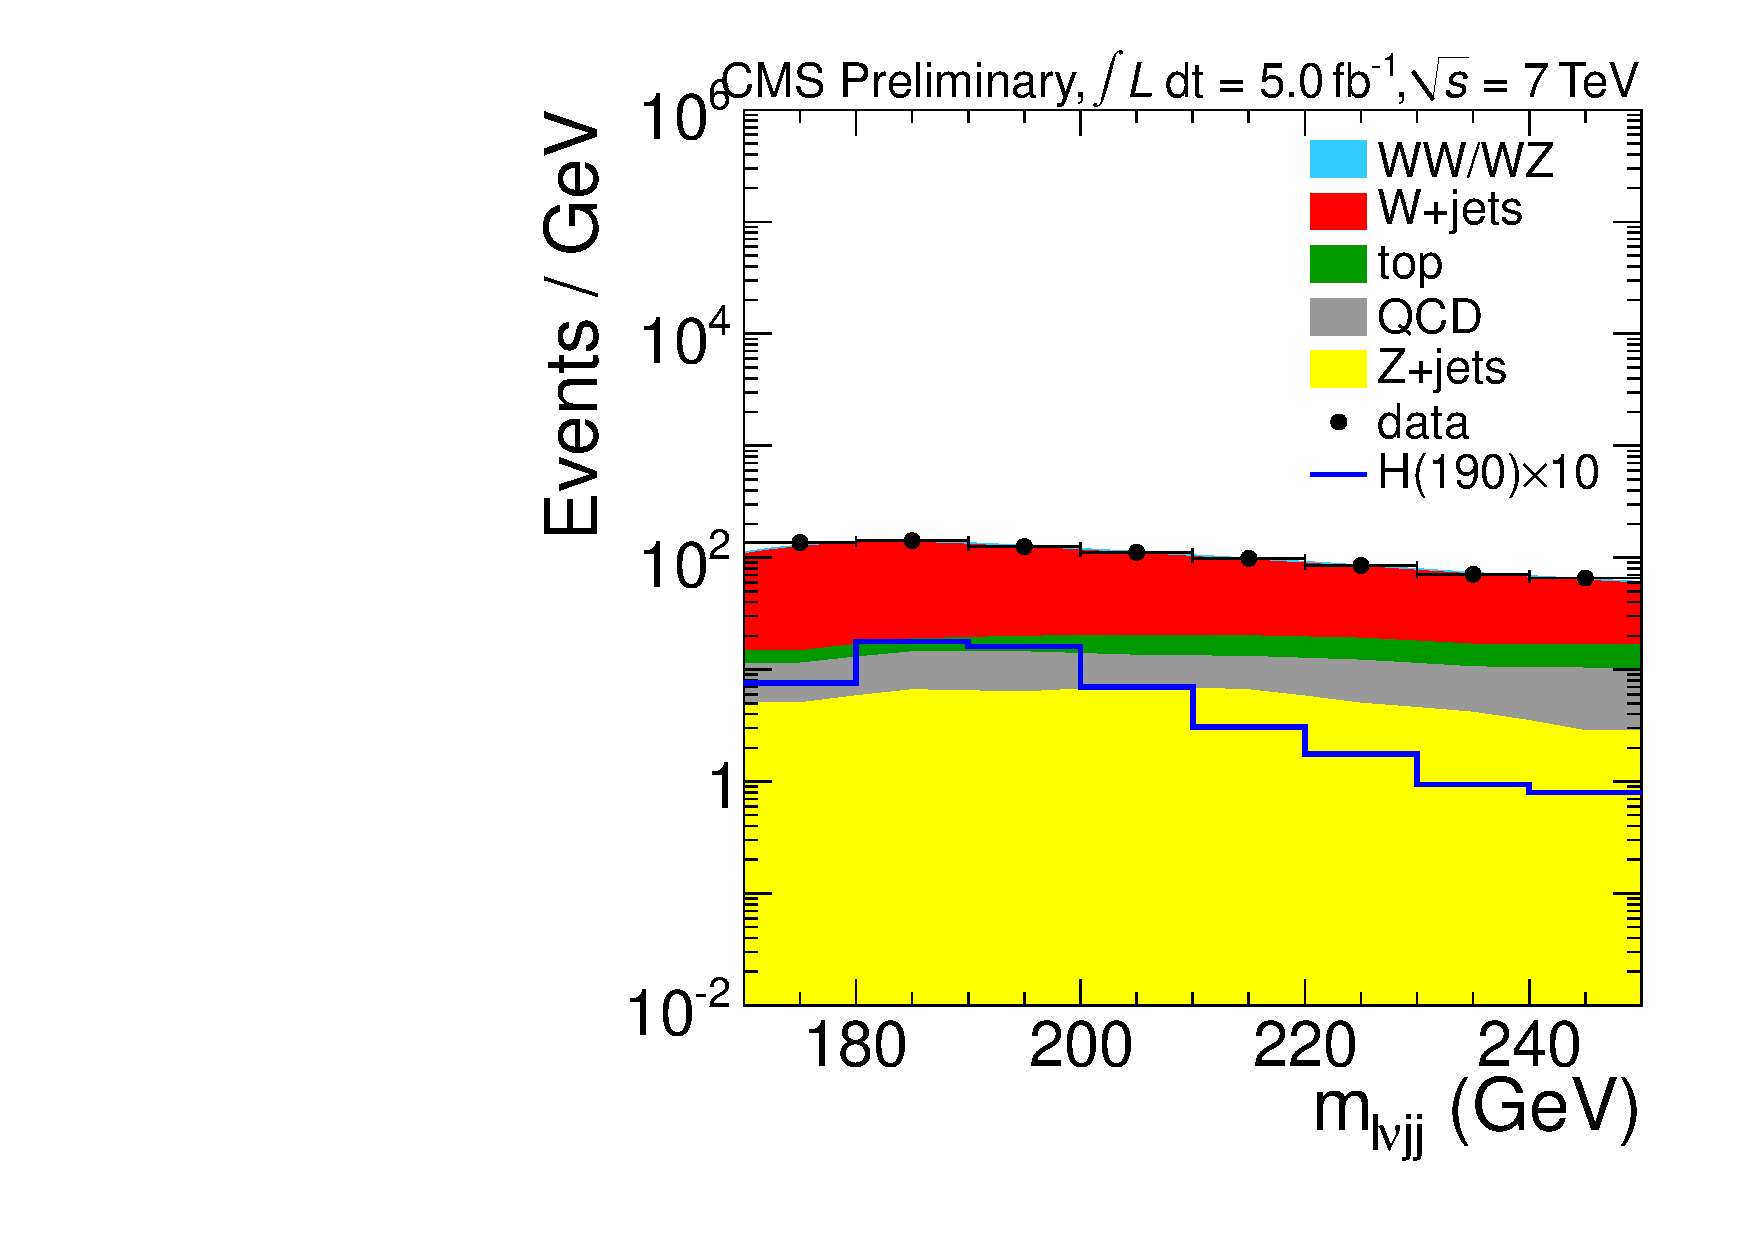
\includegraphics[width=0.3\textwidth]{plots/2012_FOURBSHAPES/H190_Mlvjj_Electron_2jets_Stacked_log}
%  }
%  \subfigure[]{
%    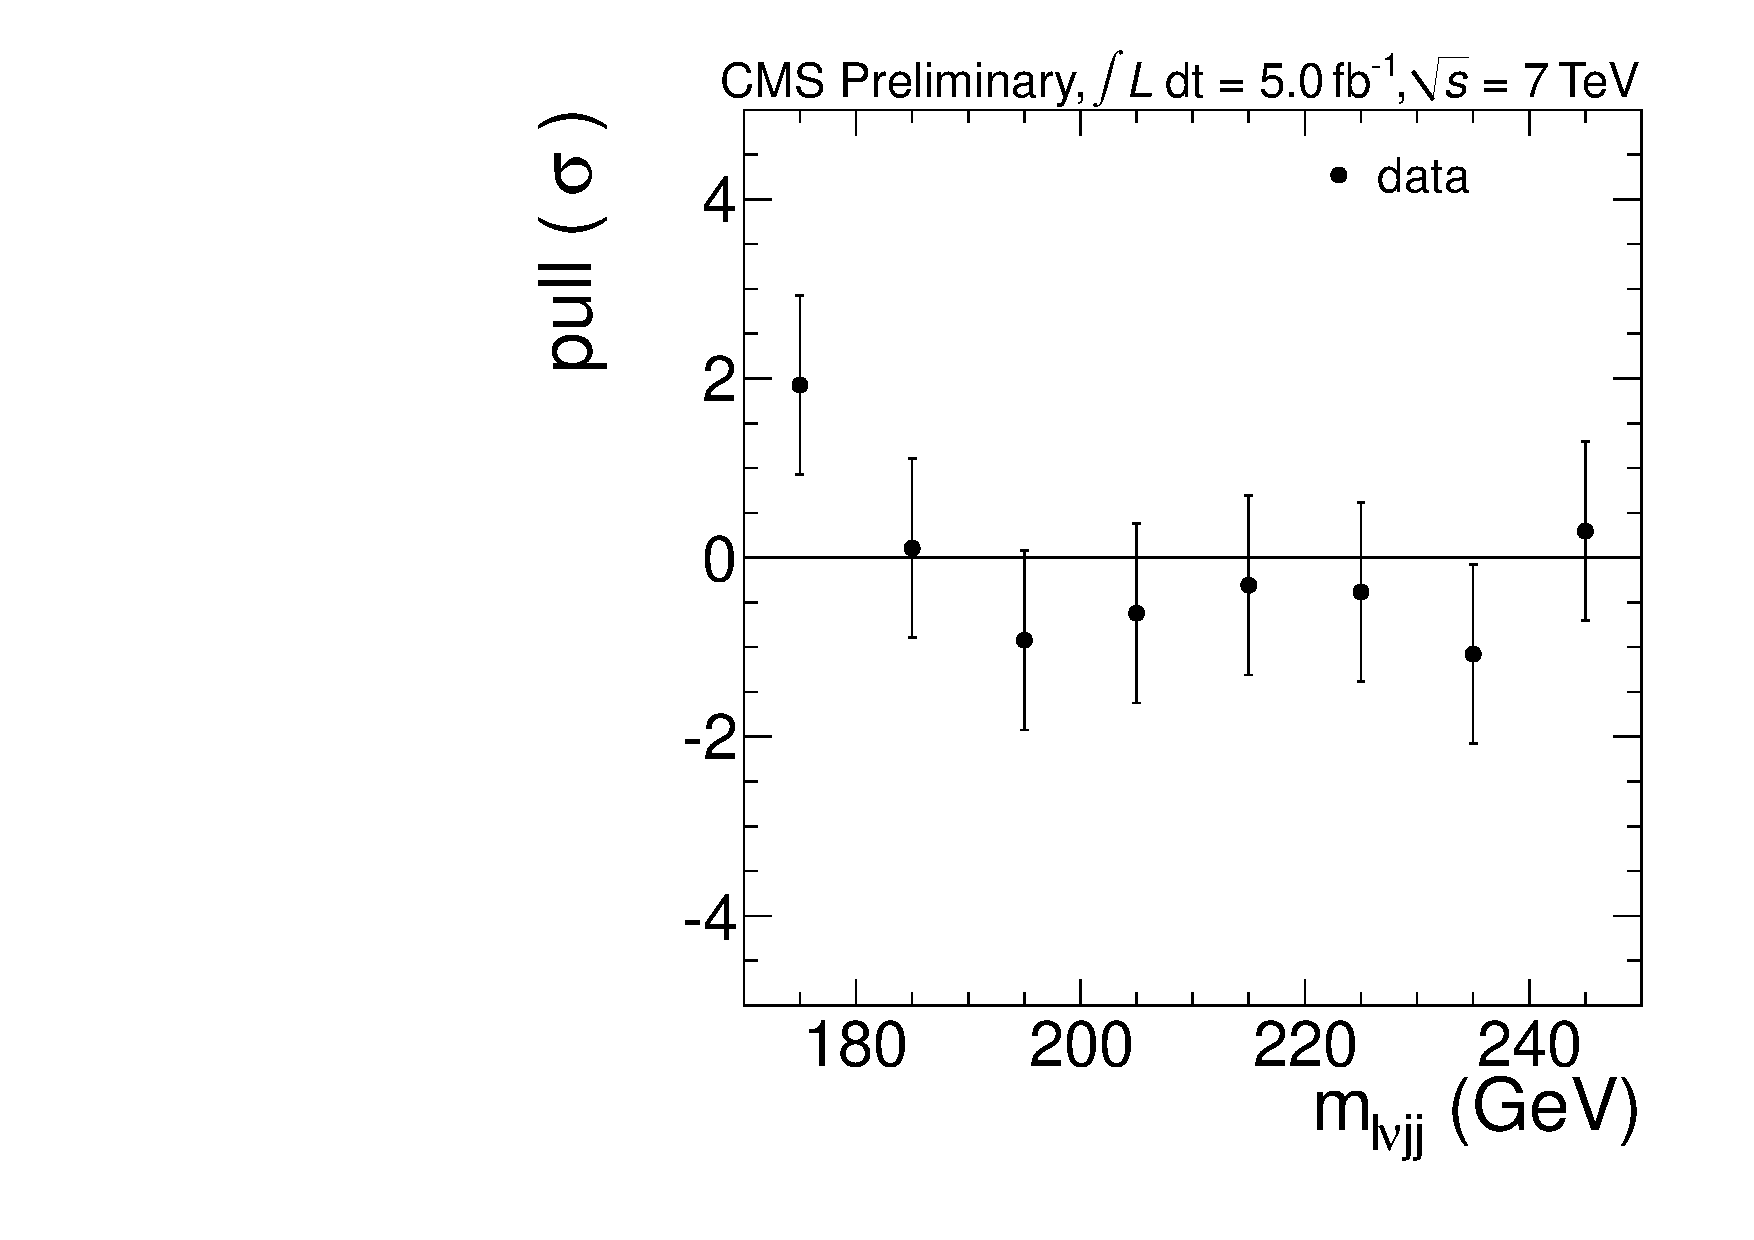
\includegraphics[width=0.3\textwidth]{plots/2012_FOURBSHAPES/H190_Mlvjj_Electron_2jets_Pull}
%  }
%  \vspace*{1mm} \\
%  \subfigure[]{
%      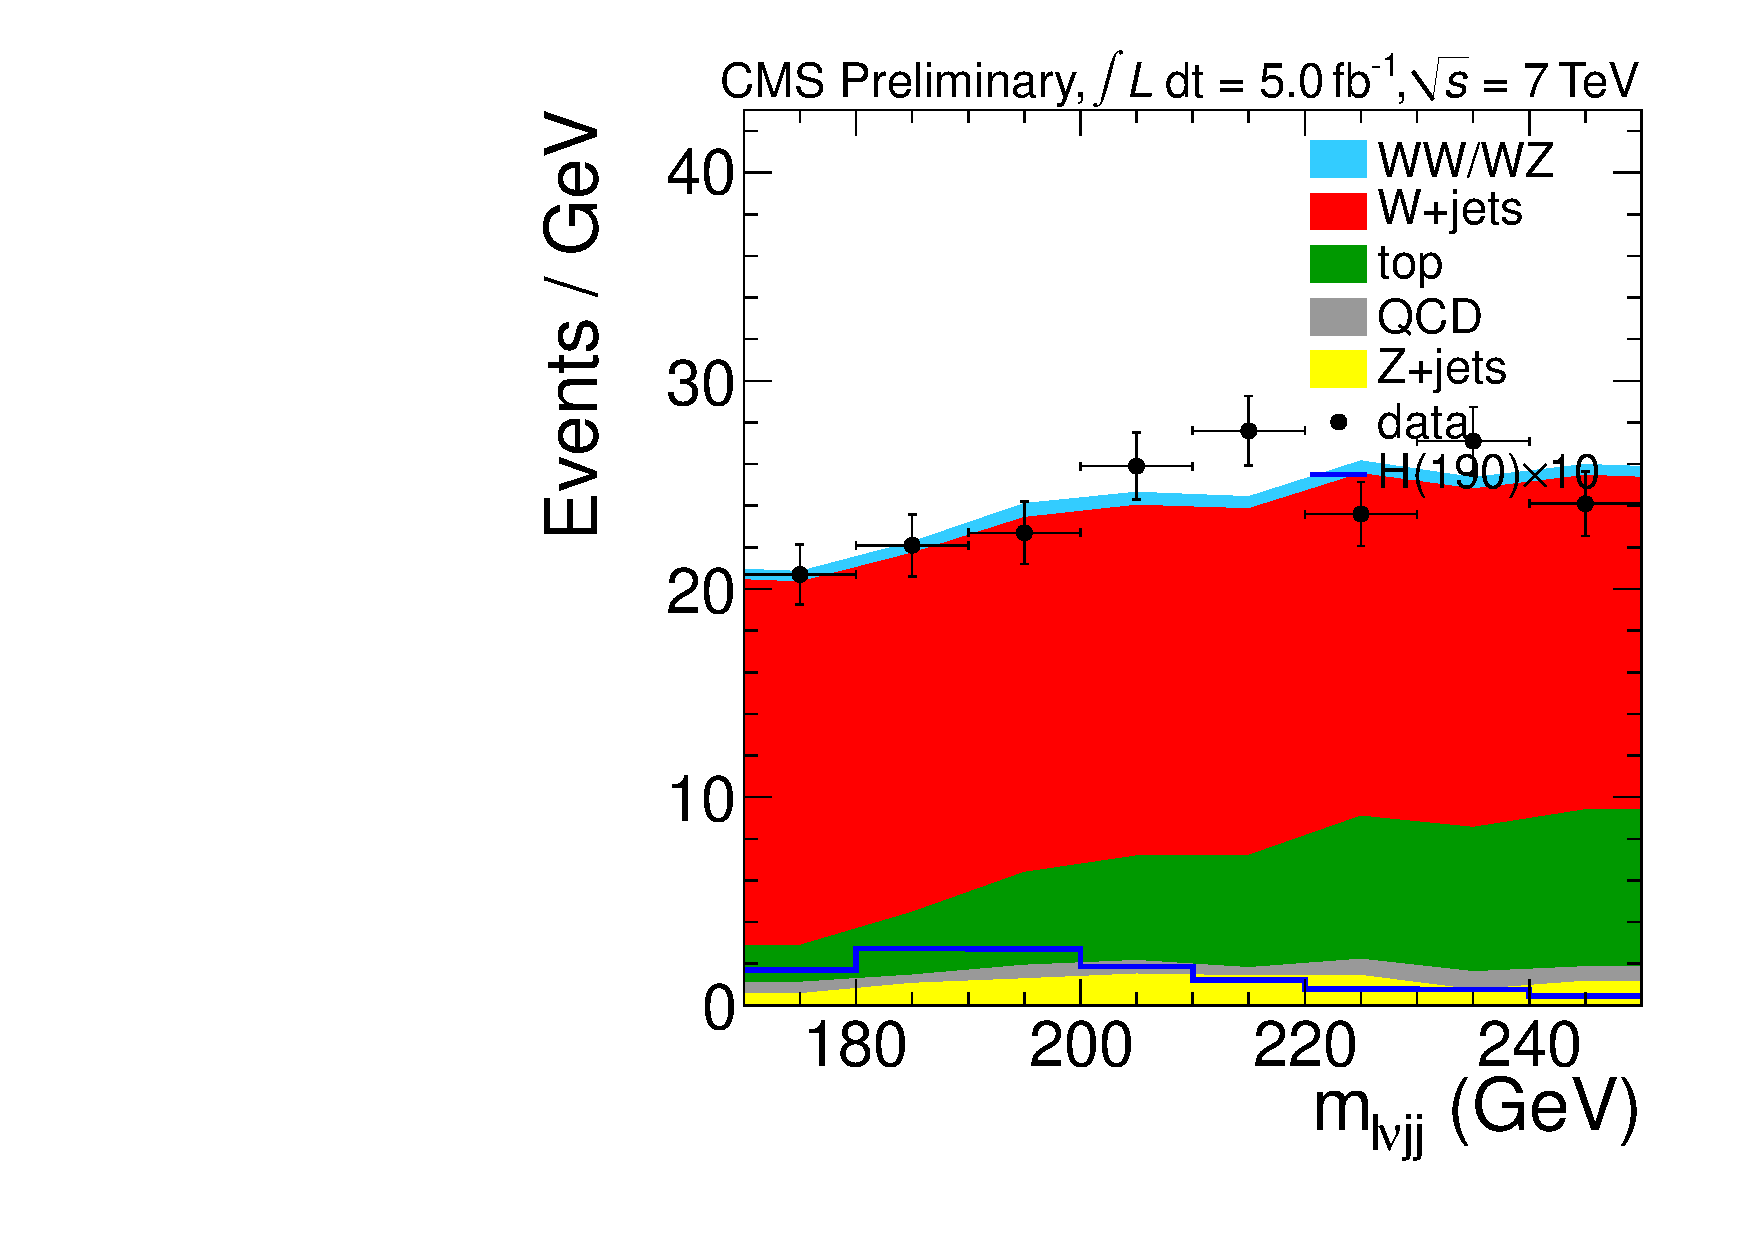
\includegraphics[width=0.3\textwidth]{plots/2012_FOURBSHAPES/H190_Mlvjj_Electron_3jets_Stacked}
%  }
%  \subfigure[]{
%    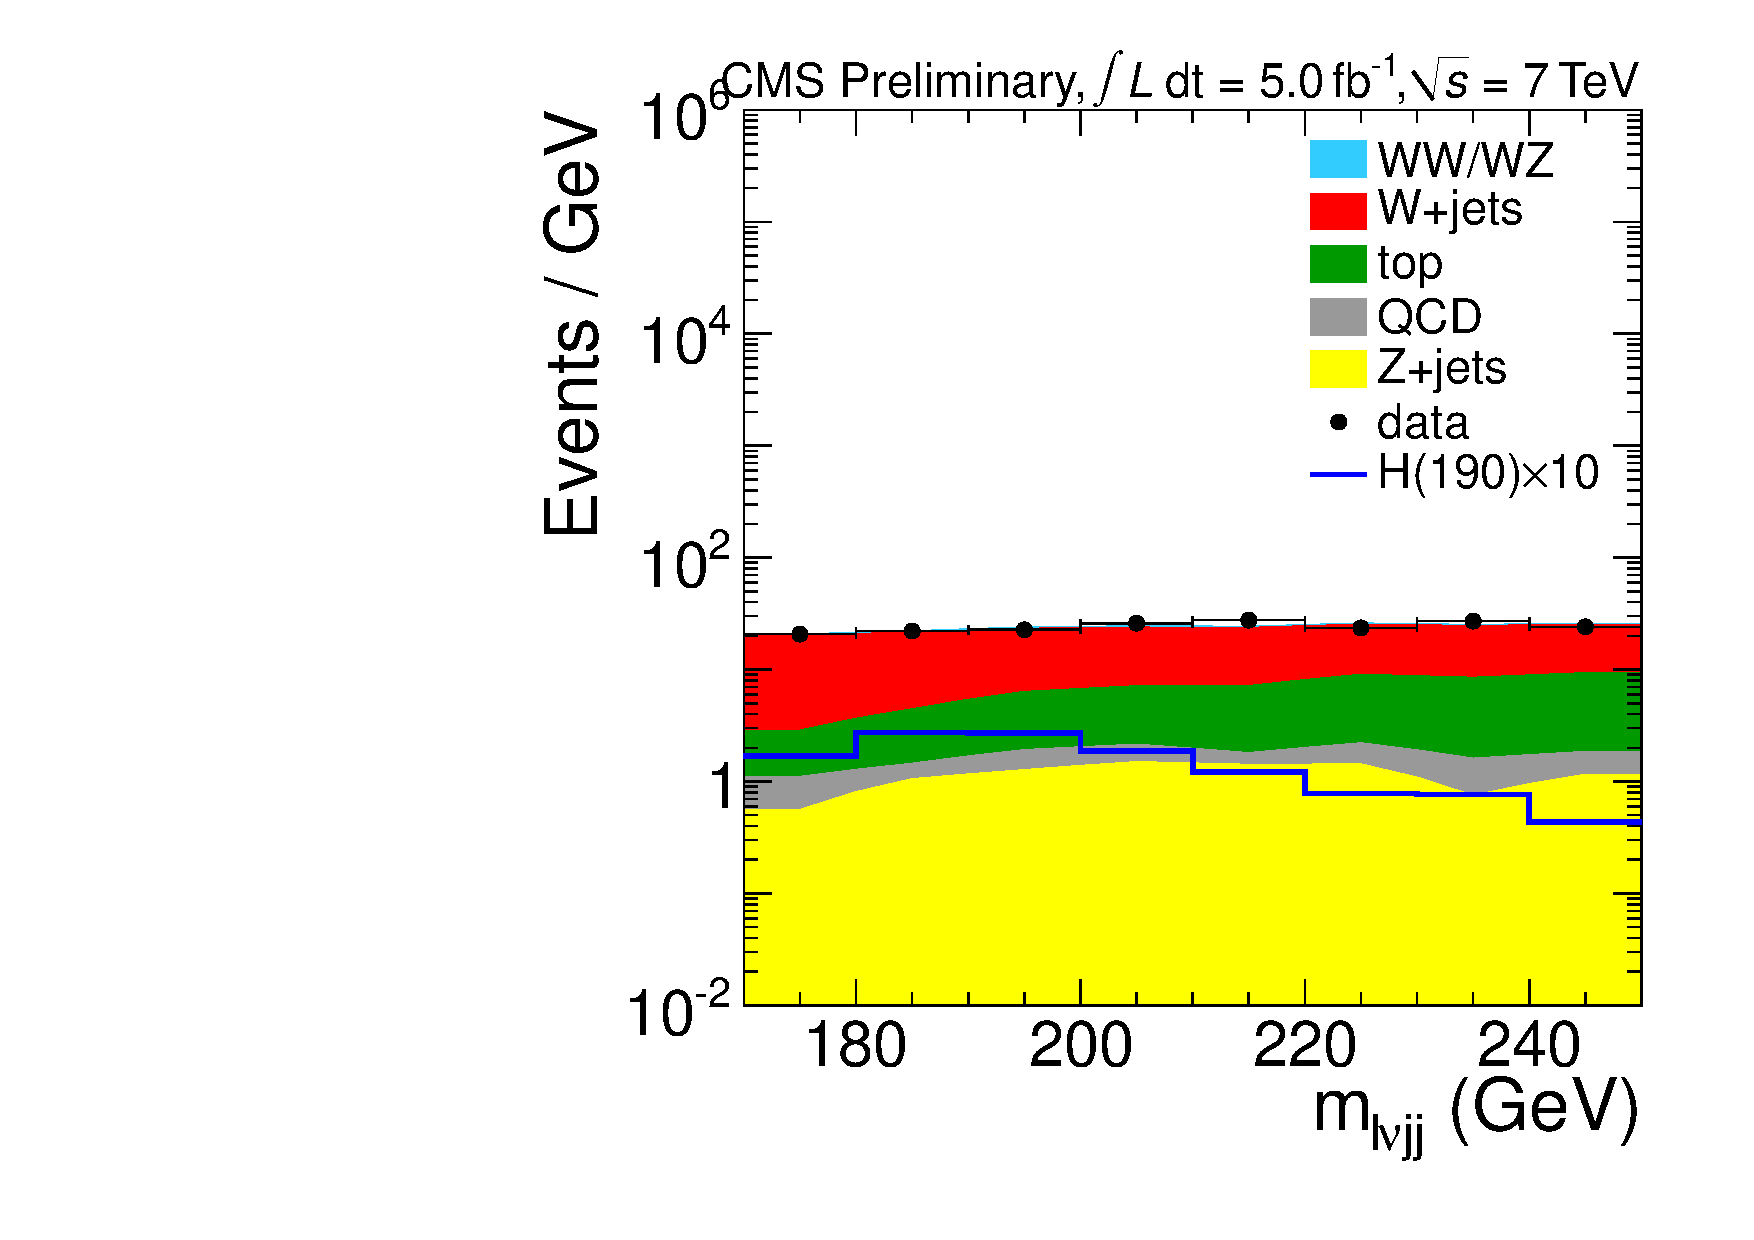
\includegraphics[width=0.3\textwidth]{plots/2012_FOURBSHAPES/H190_Mlvjj_Electron_3jets_Stacked_log}
%  }
%  \subfigure[]{
%    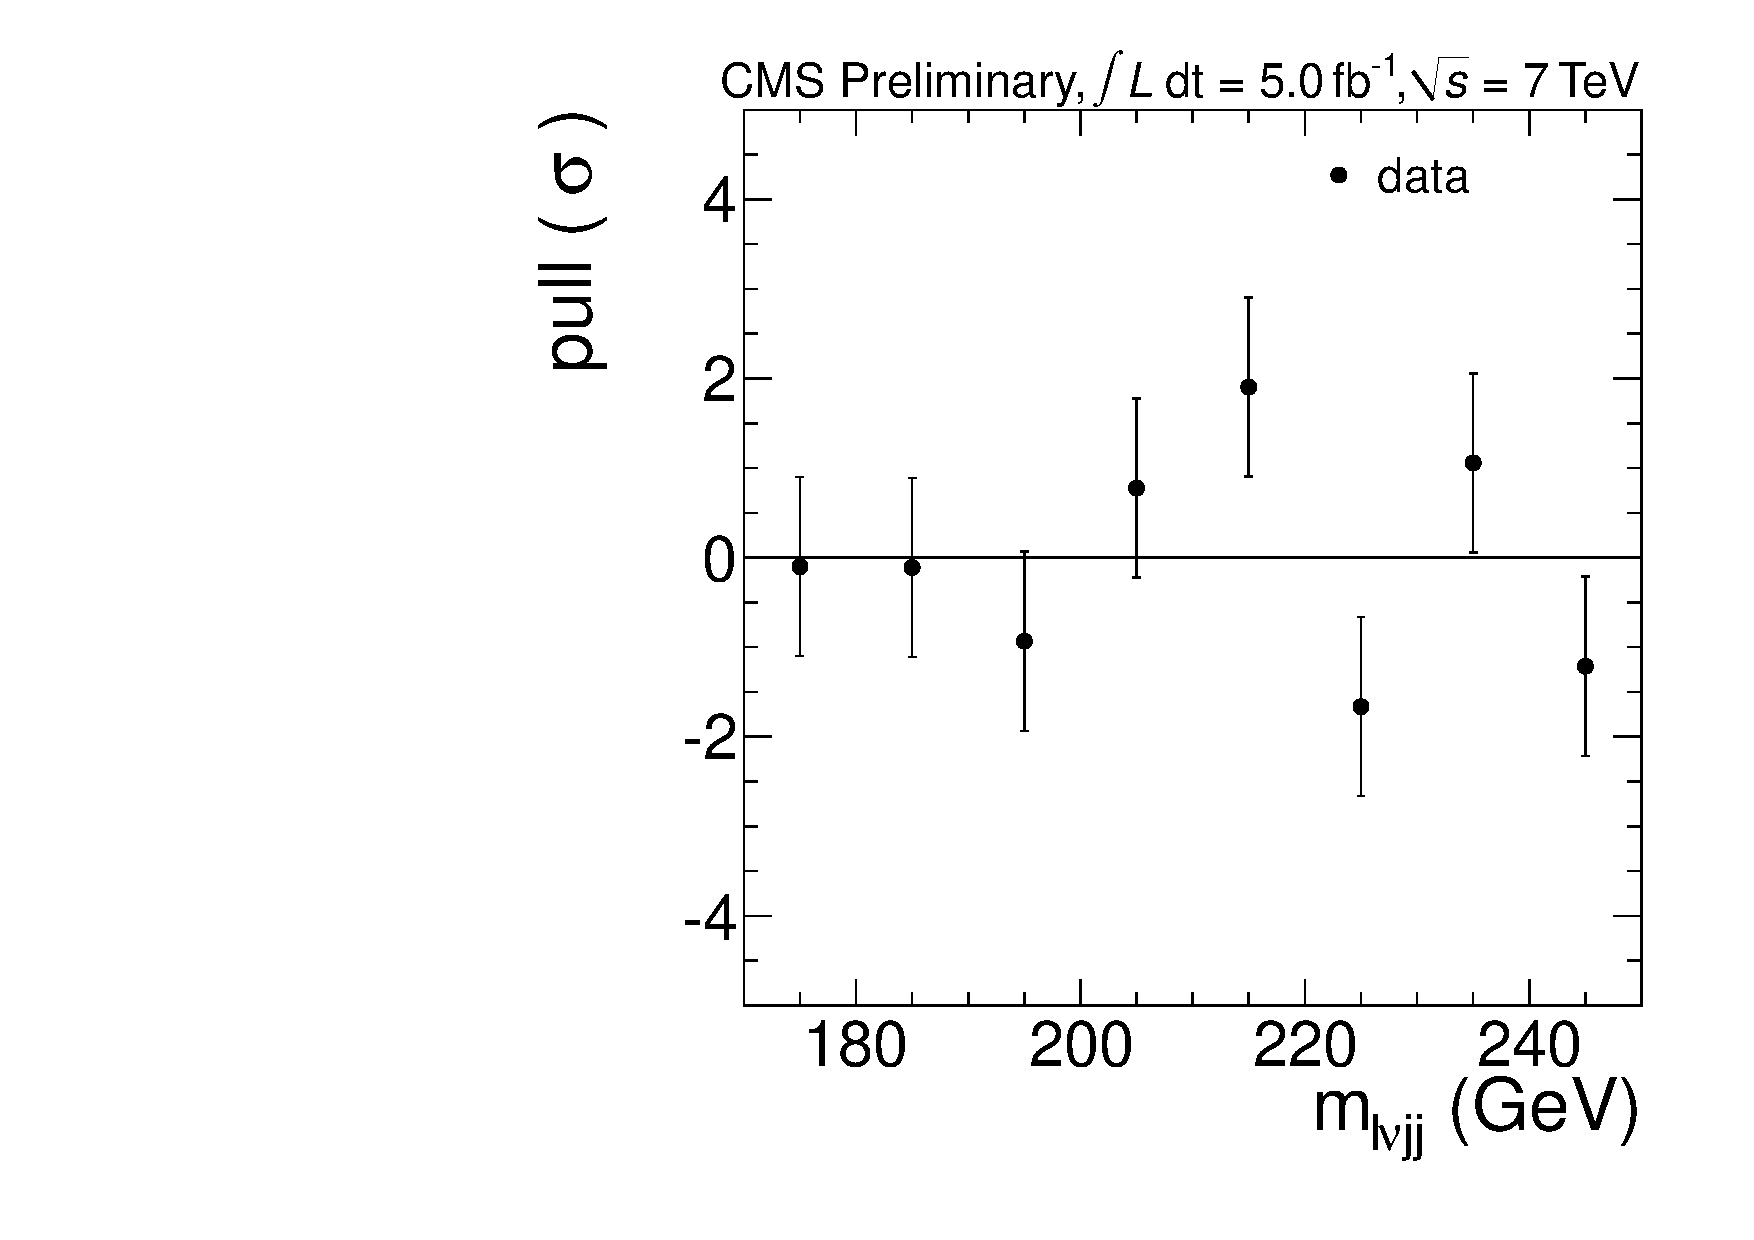
\includegraphics[width=0.3\textwidth]{plots/2012_FOURBSHAPES/H190_Mlvjj_Electron_3jets_Pull}
%  }
%  \caption{$M_H = 190$~GeV point. The distribution of the 4-body invariant mass $m_{\ell\nu jj}$ plotted on 
%  linear (left) and log (center) scales. The pull distribution computed as 
%  [(Data - Background)/ Background uncertainty] is shown on the right.
%  The four rows correspond to muon 2-jets, muon 3-jets, electron 2-jets, 
%  and electron 3-jets event categories, respectively. }
%  \label{fig:mlnujj_mH190}
%  \end{figure}
%%%%%%%%%%%%%%%%%%%%
%%%%%%%%%%%%%%%%%%%%
%%%%%%%%%%%%%%%%%%%%
% \begin{figure}[h!t]
% \subfigure[]{
%     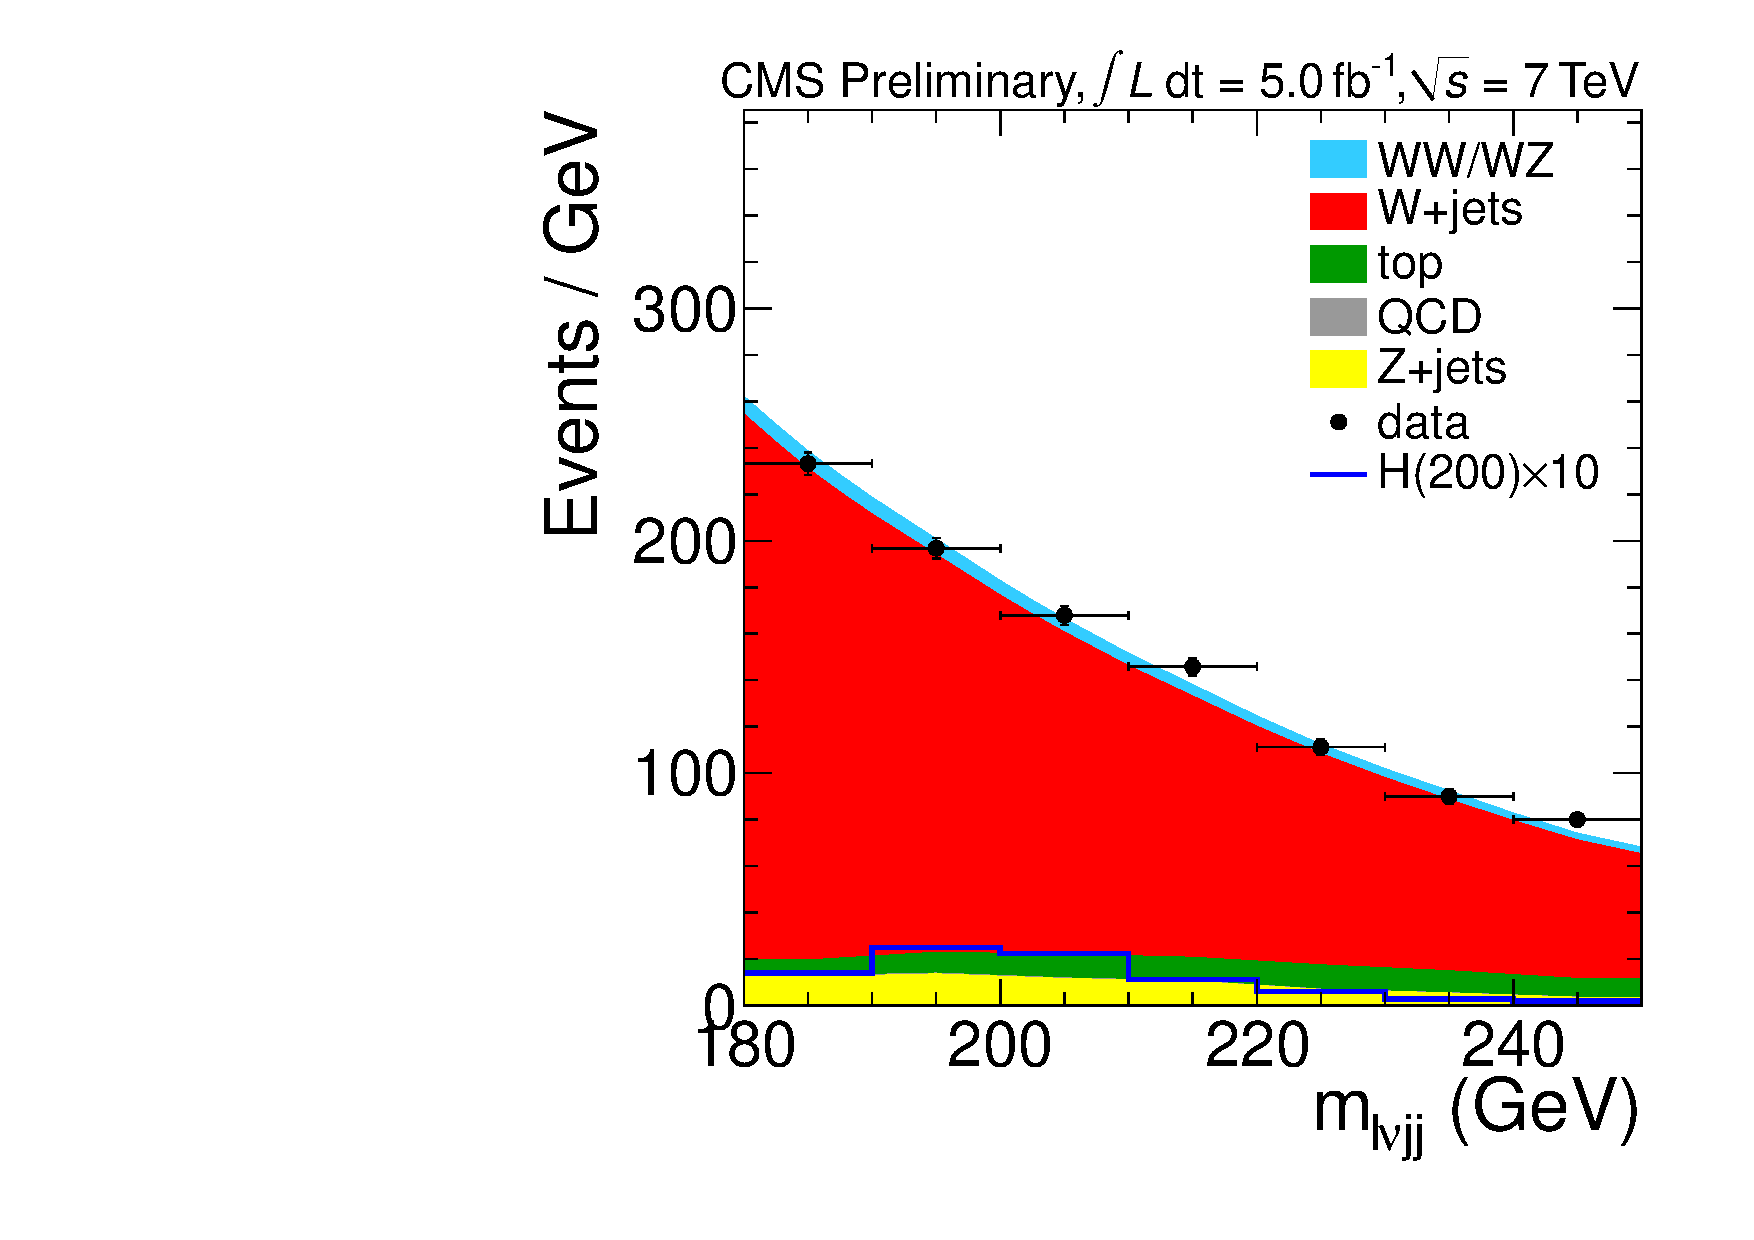
\includegraphics[width=0.3\textwidth]{plots/2012_FOURBSHAPES/H200_Mlvjj_Muon_2jets_Stacked}
% }
% \subfigure[]{
%   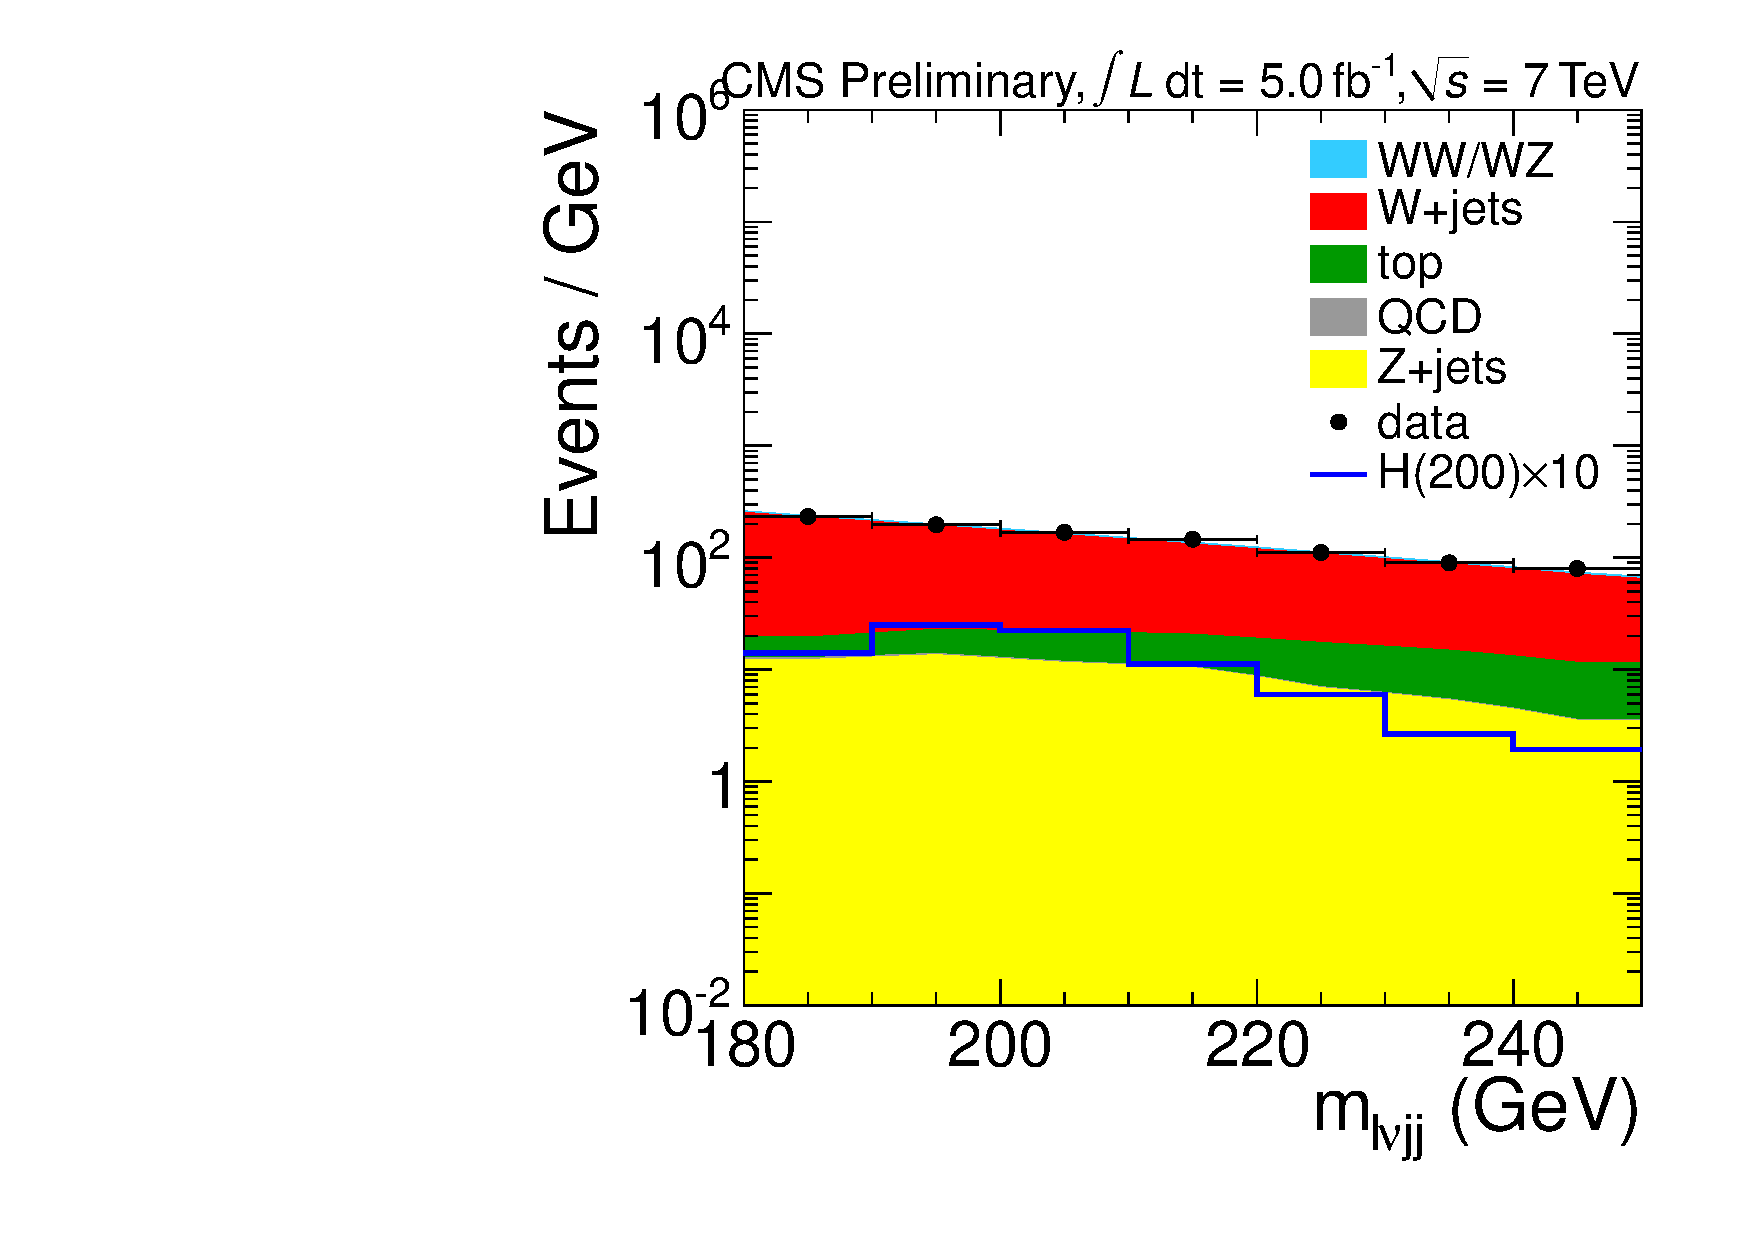
\includegraphics[width=0.3\textwidth]{plots/2012_FOURBSHAPES/H200_Mlvjj_Muon_2jets_Stacked_log}
% }
% \subfigure[]{
%   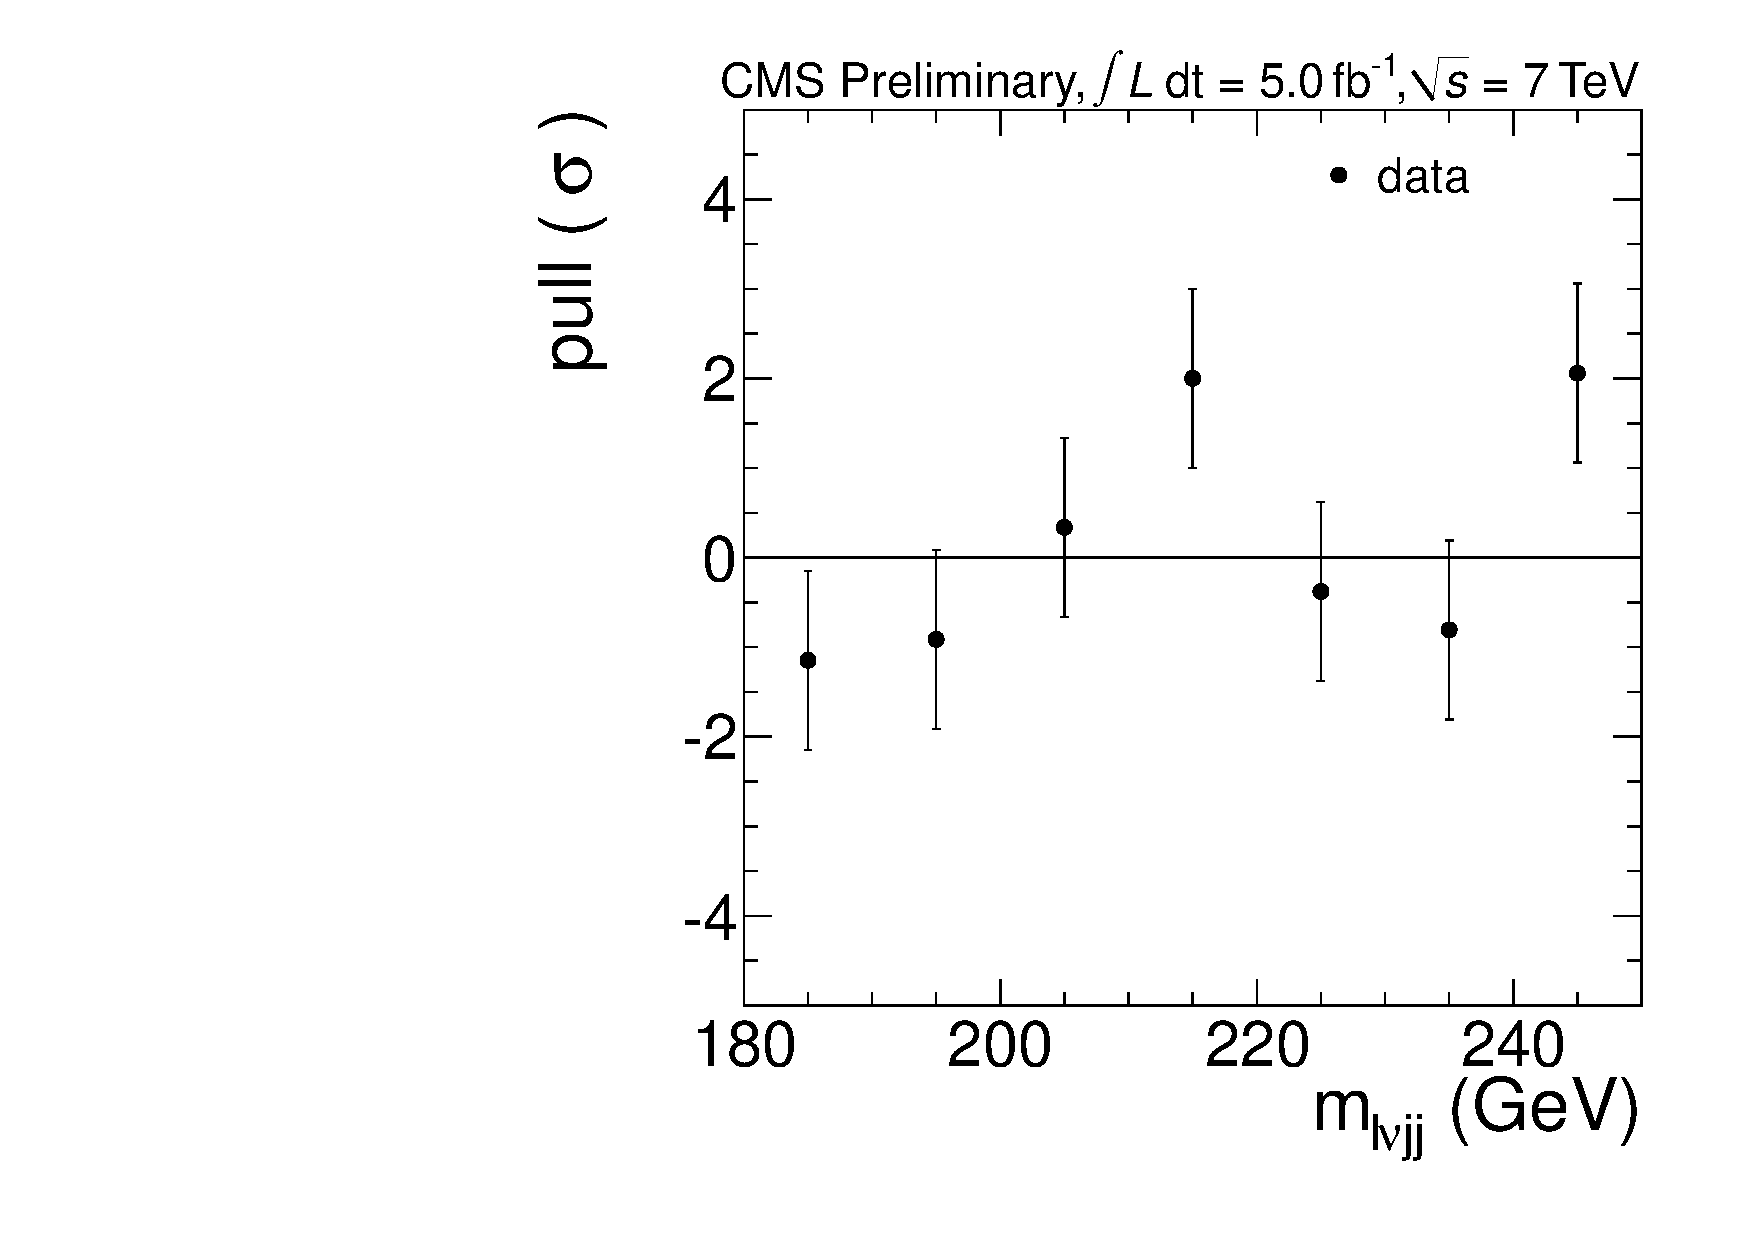
\includegraphics[width=0.3\textwidth]{plots/2012_FOURBSHAPES/H200_Mlvjj_Muon_2jets_Pull}
% }
% \vspace*{1mm} \\
% \subfigure[]{
%     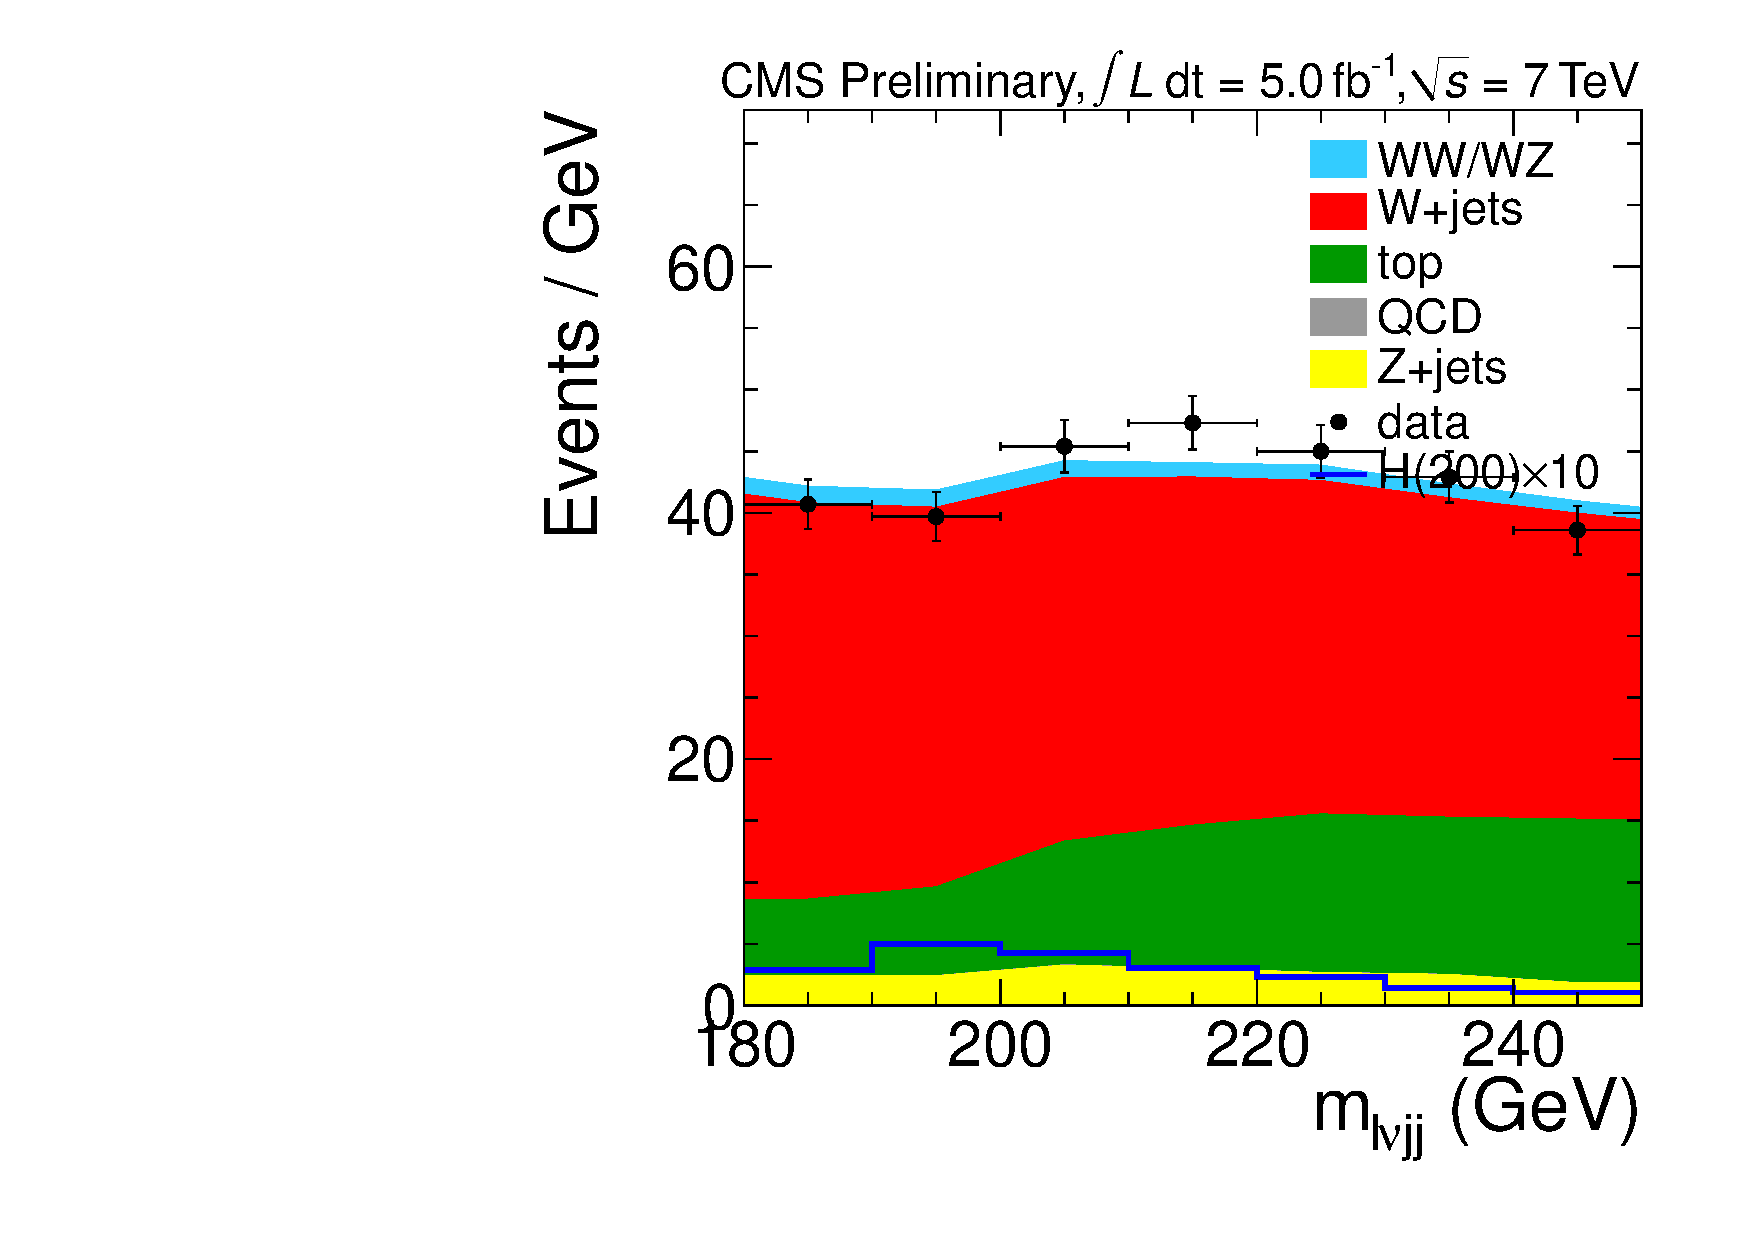
\includegraphics[width=0.3\textwidth]{plots/2012_FOURBSHAPES/H200_Mlvjj_Muon_3jets_Stacked}
% }
% \subfigure[]{
%   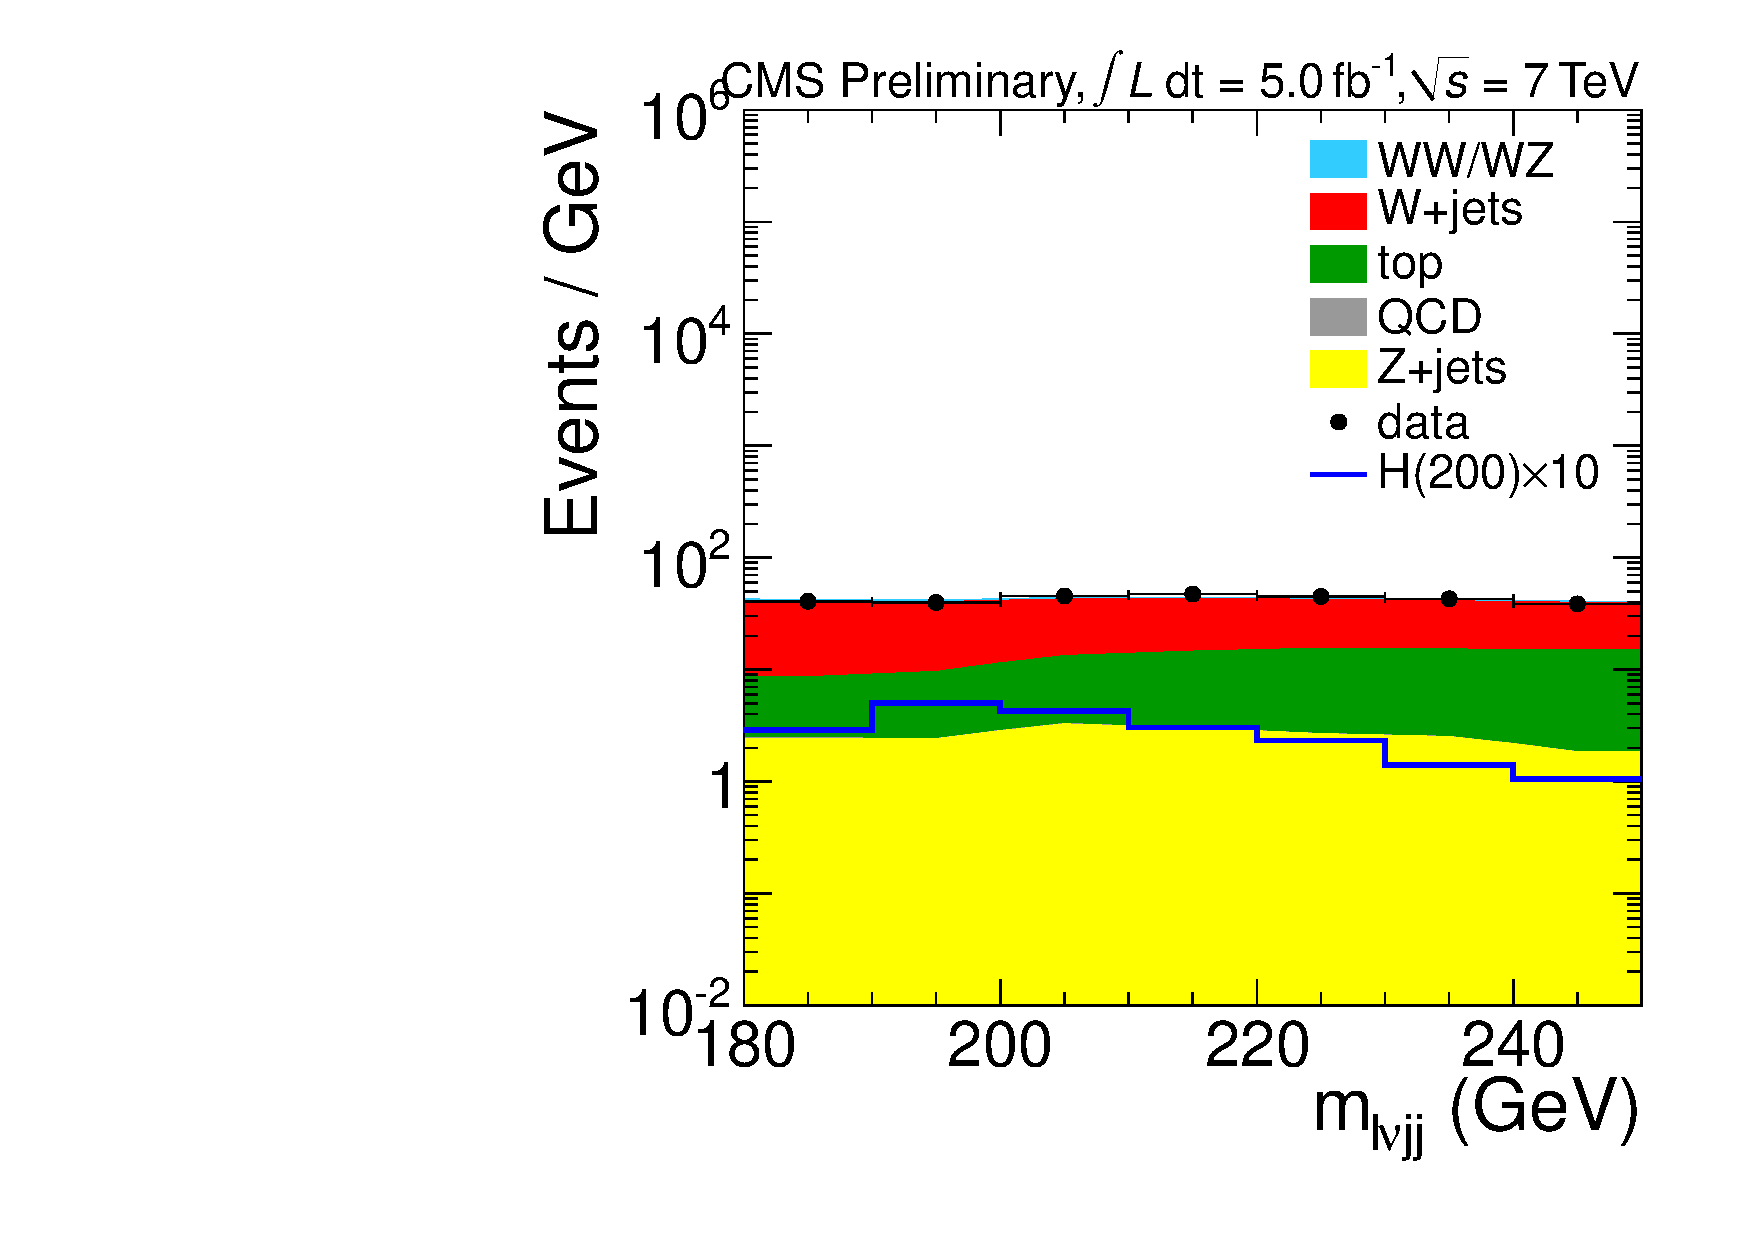
\includegraphics[width=0.3\textwidth]{plots/2012_FOURBSHAPES/H200_Mlvjj_Muon_3jets_Stacked_log}
% }
% \subfigure[]{
%   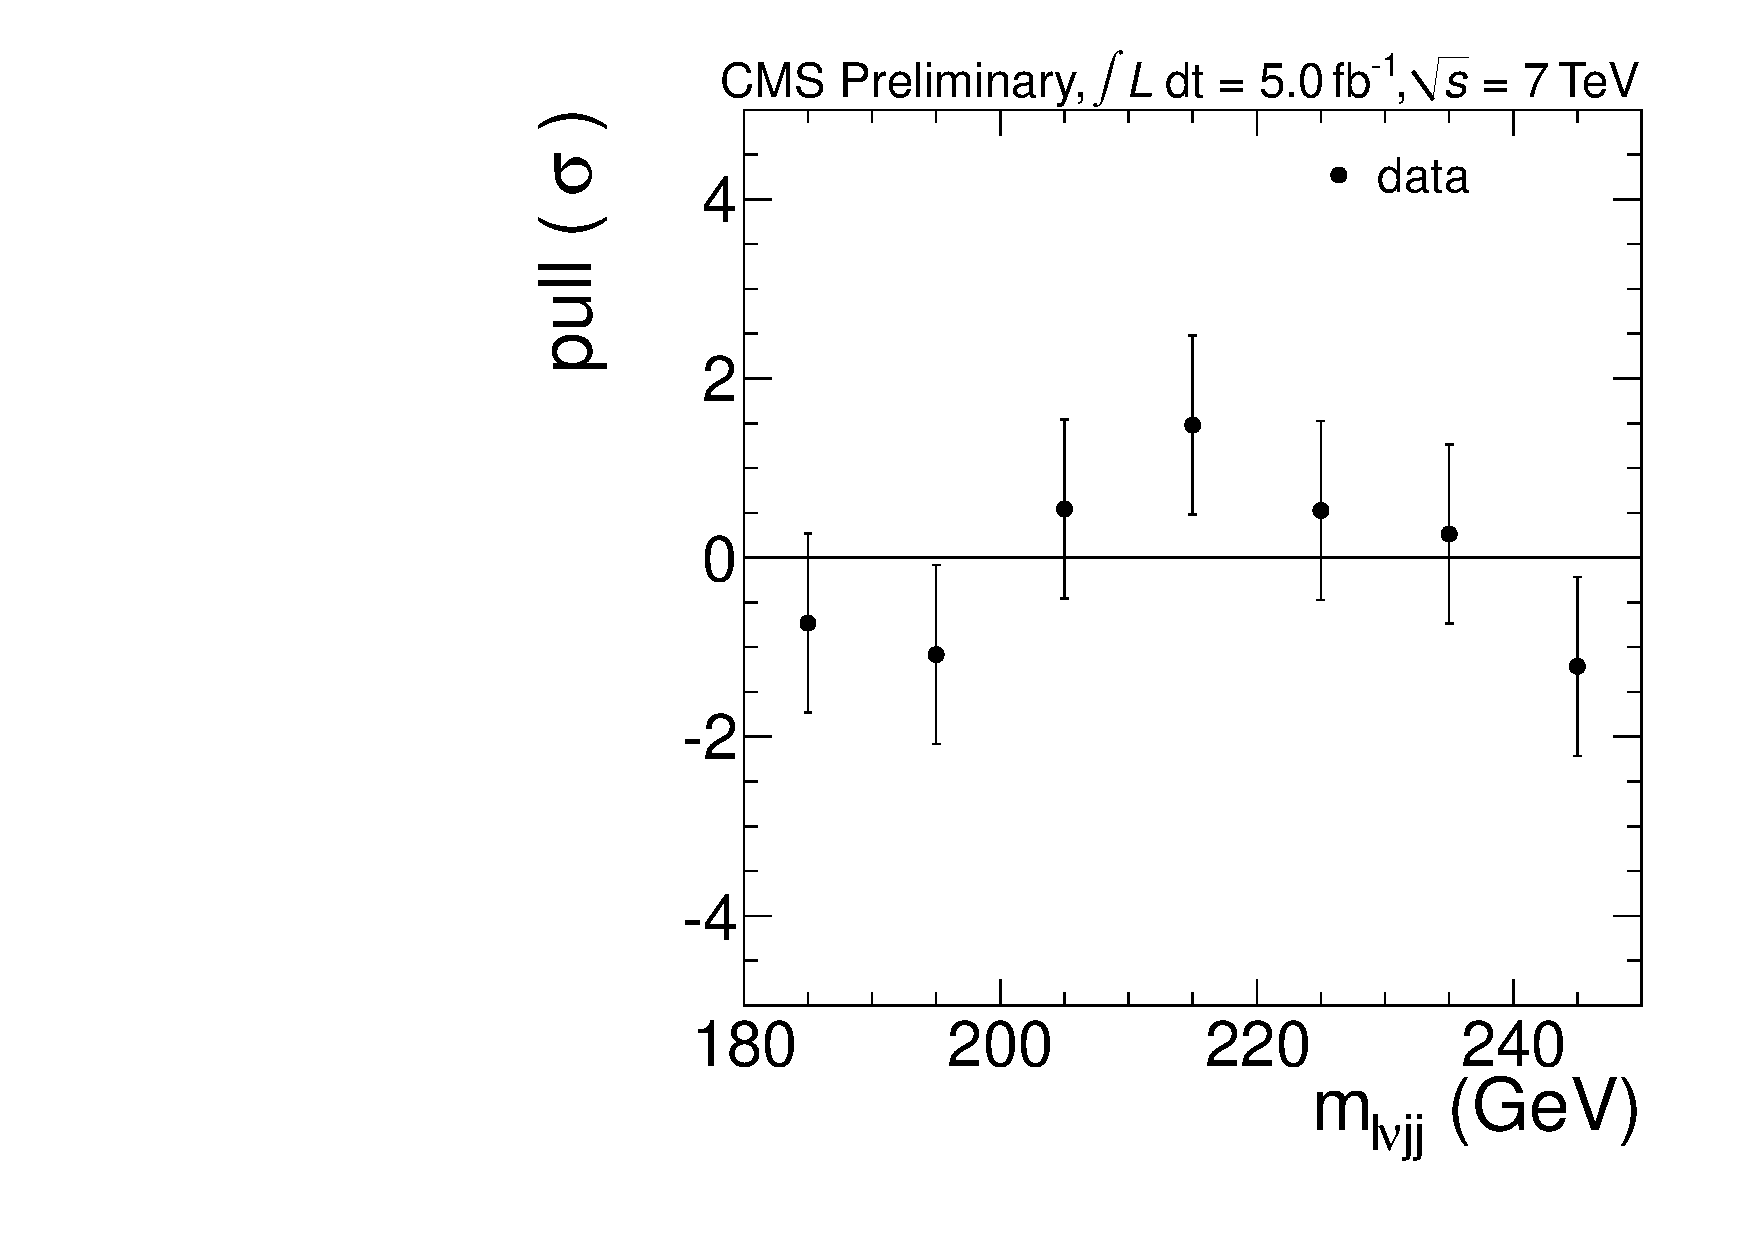
\includegraphics[width=0.3\textwidth]{plots/2012_FOURBSHAPES/H200_Mlvjj_Muon_3jets_Pull}
% }
% \vspace*{1mm} \\
% \subfigure[]{
%     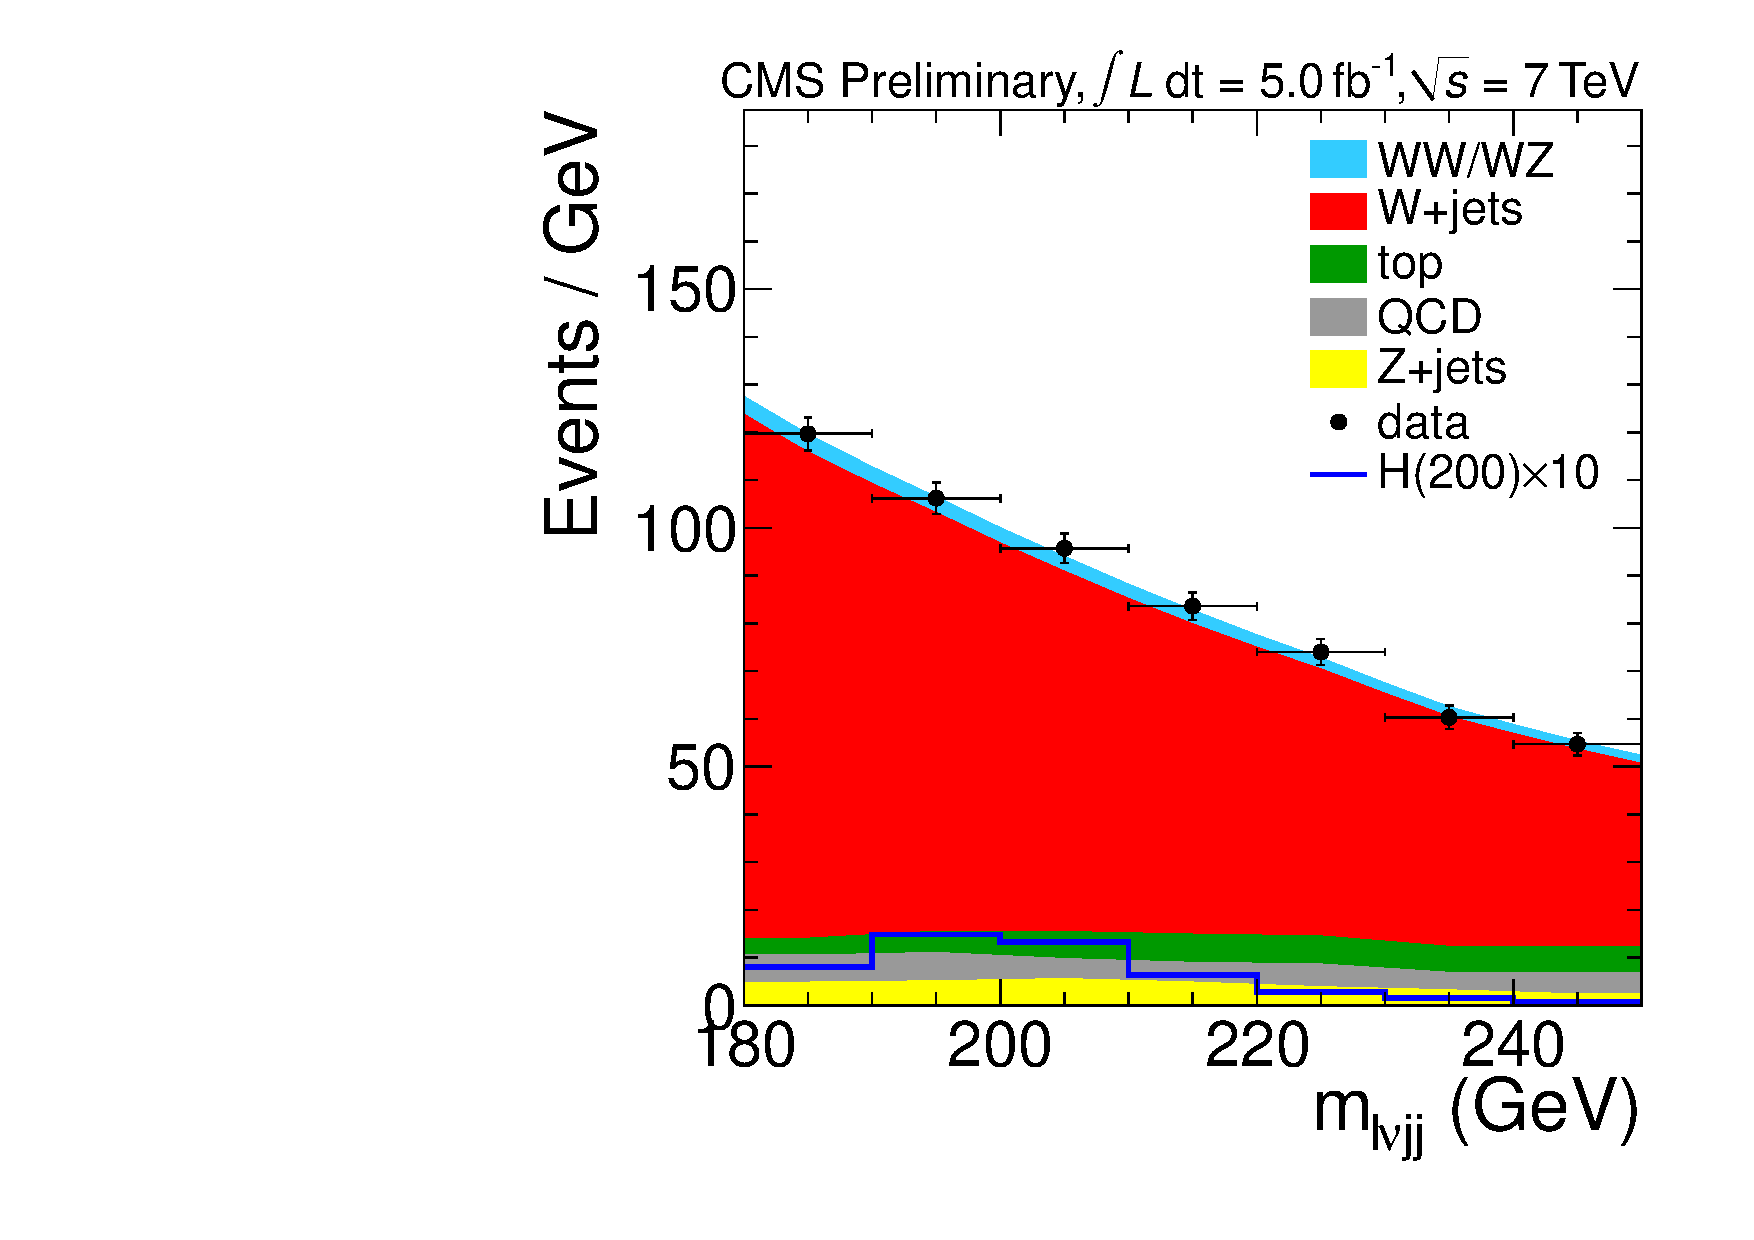
\includegraphics[width=0.3\textwidth]{plots/2012_FOURBSHAPES/H200_Mlvjj_Electron_2jets_Stacked}
% }
% \subfigure[]{
%   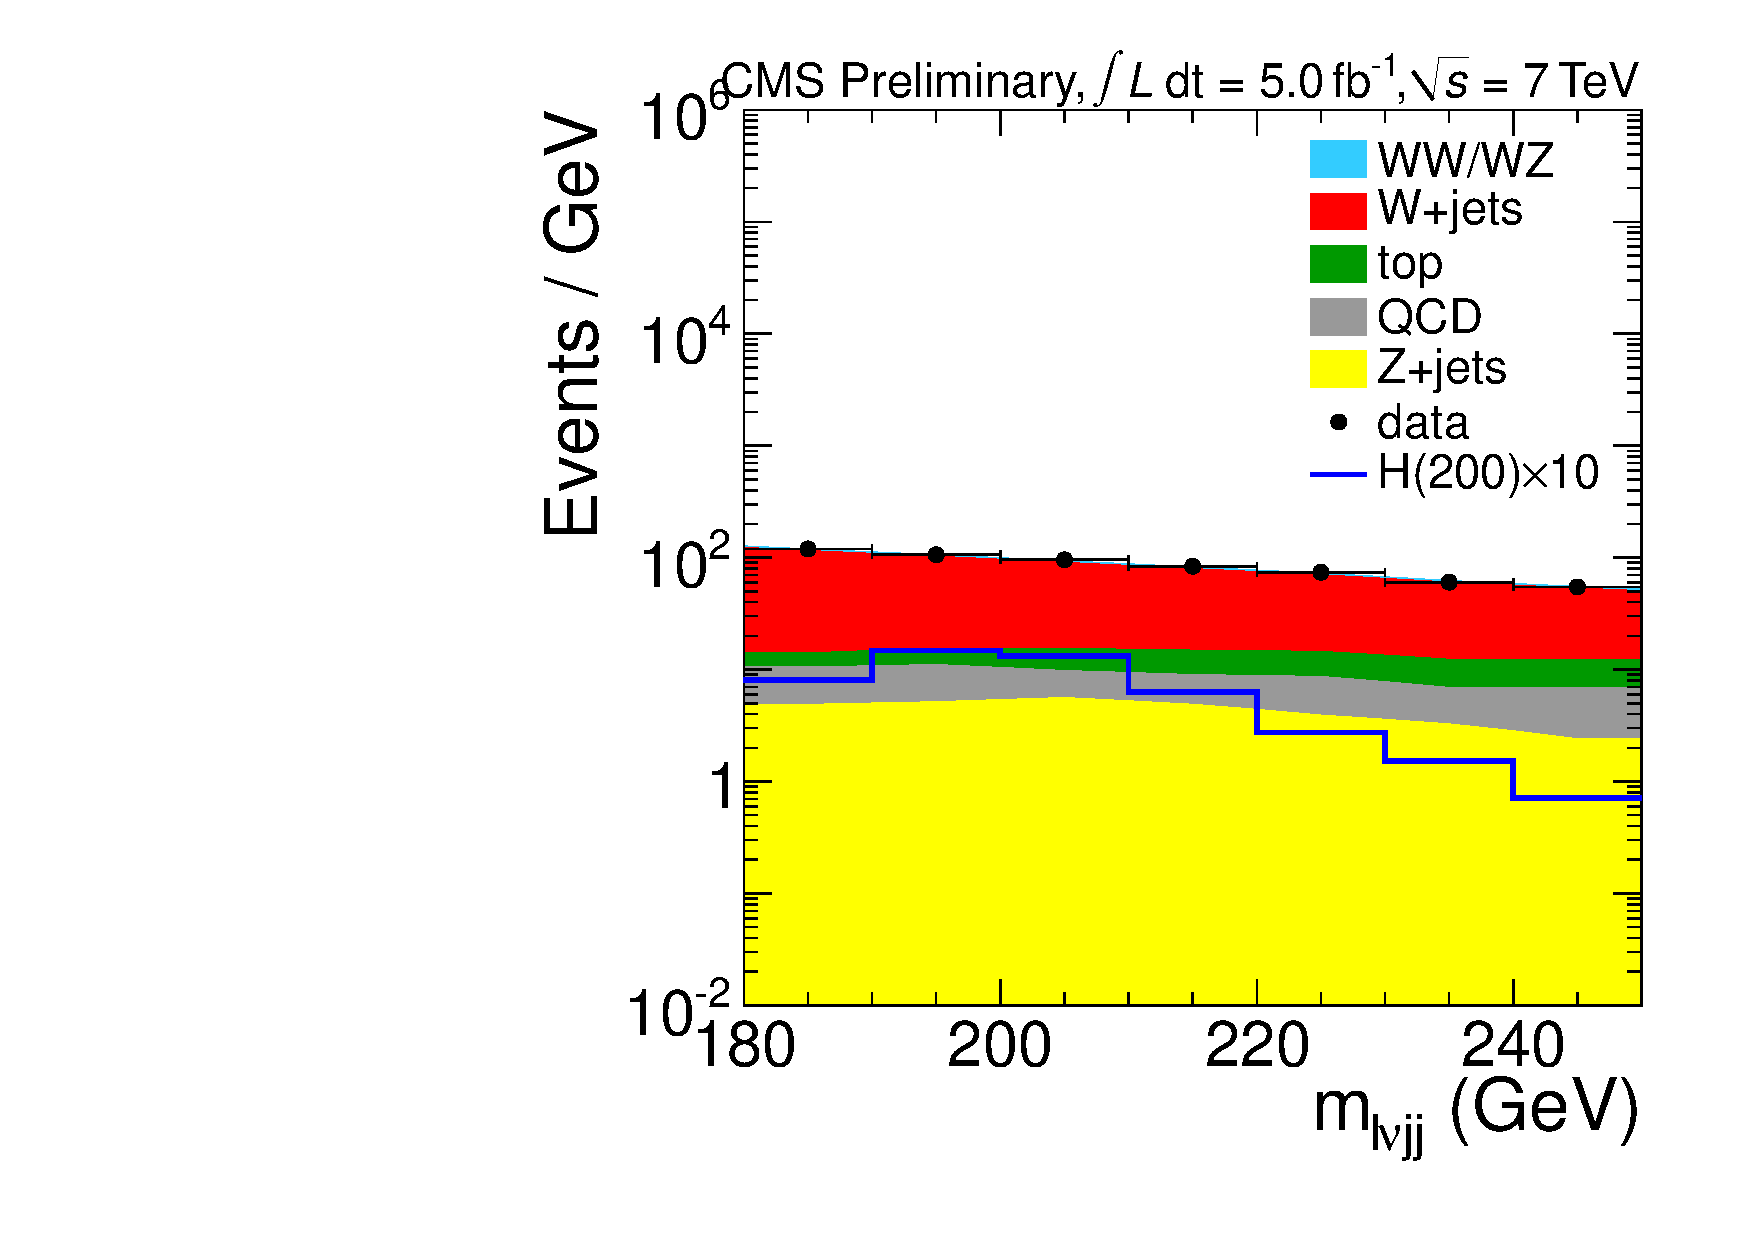
\includegraphics[width=0.3\textwidth]{plots/2012_FOURBSHAPES/H200_Mlvjj_Electron_2jets_Stacked_log}
% }
% \subfigure[]{
%   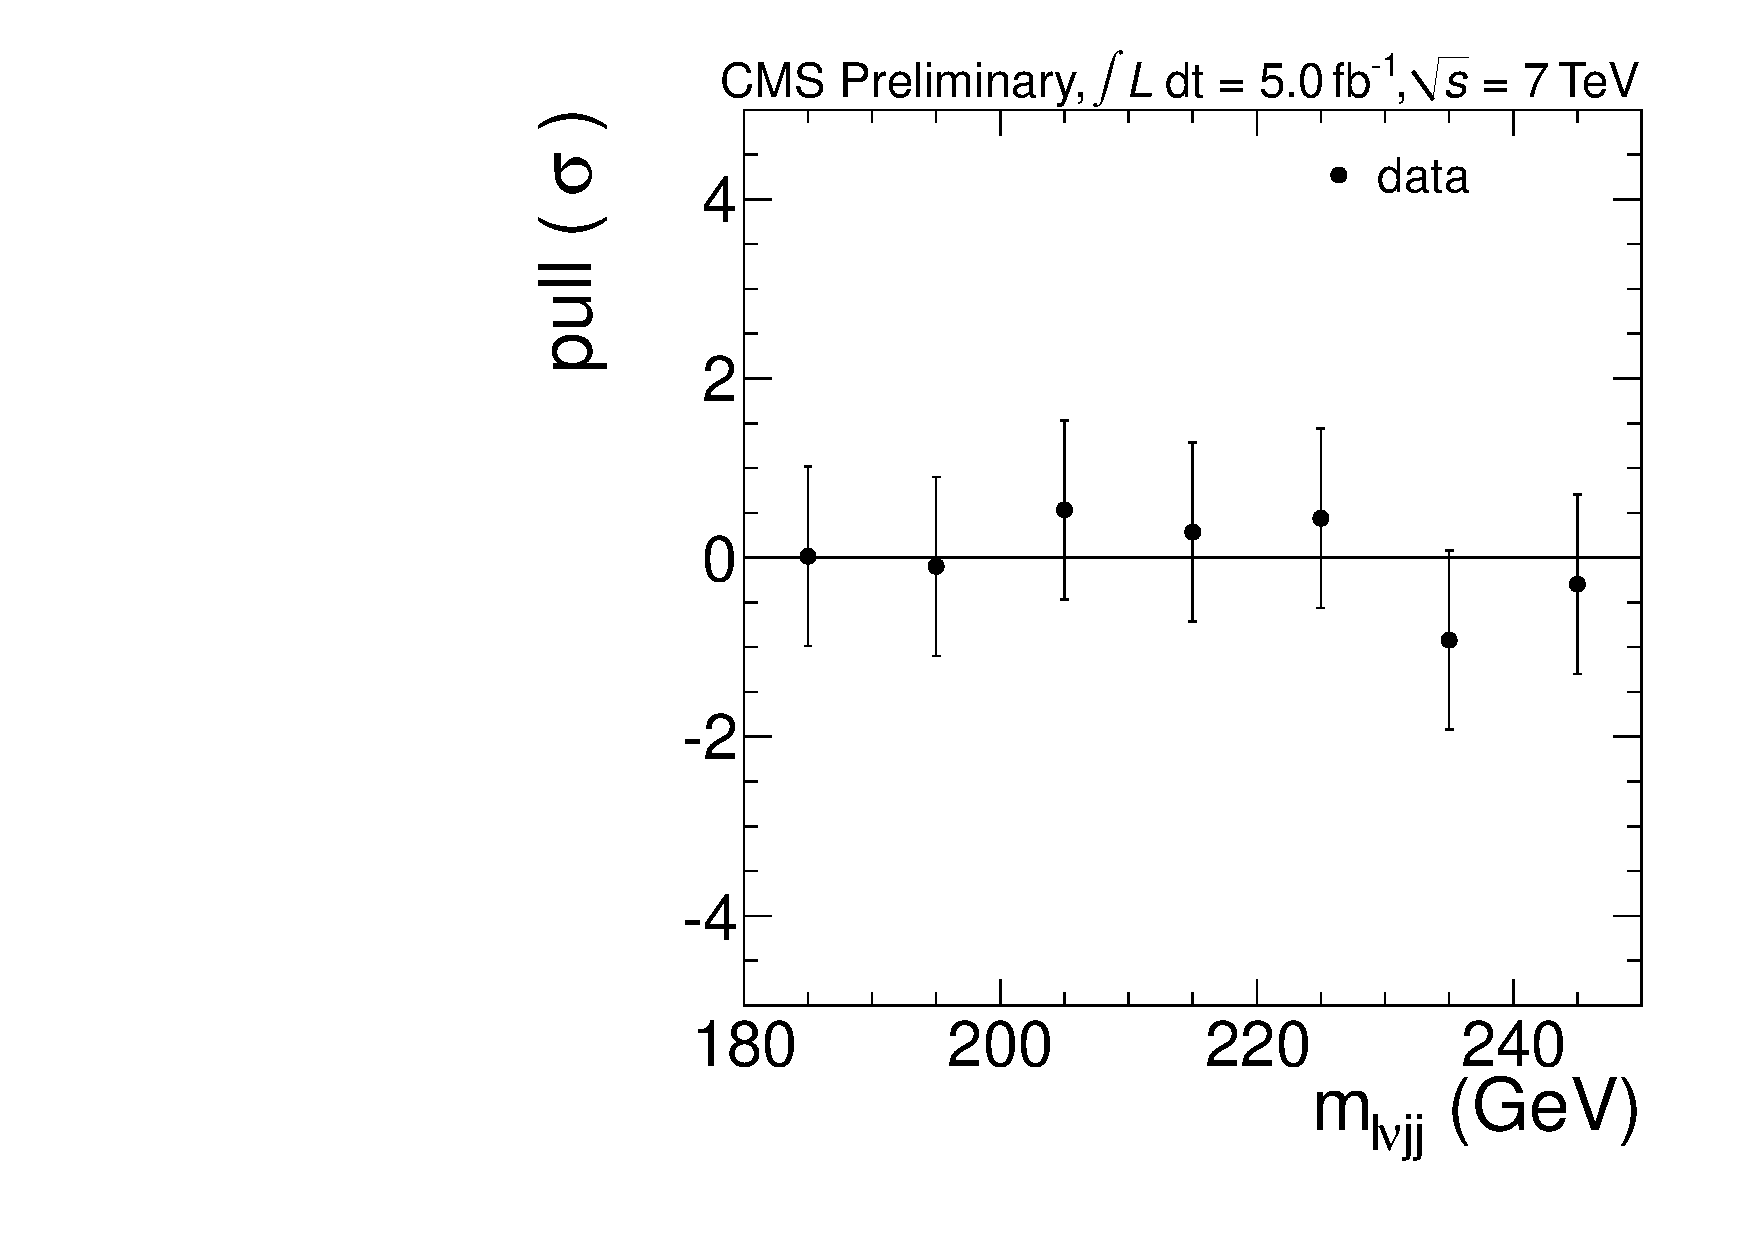
\includegraphics[width=0.3\textwidth]{plots/2012_FOURBSHAPES/H200_Mlvjj_Electron_2jets_Pull}
% }
% \vspace*{1mm} \\
% \subfigure[]{
%     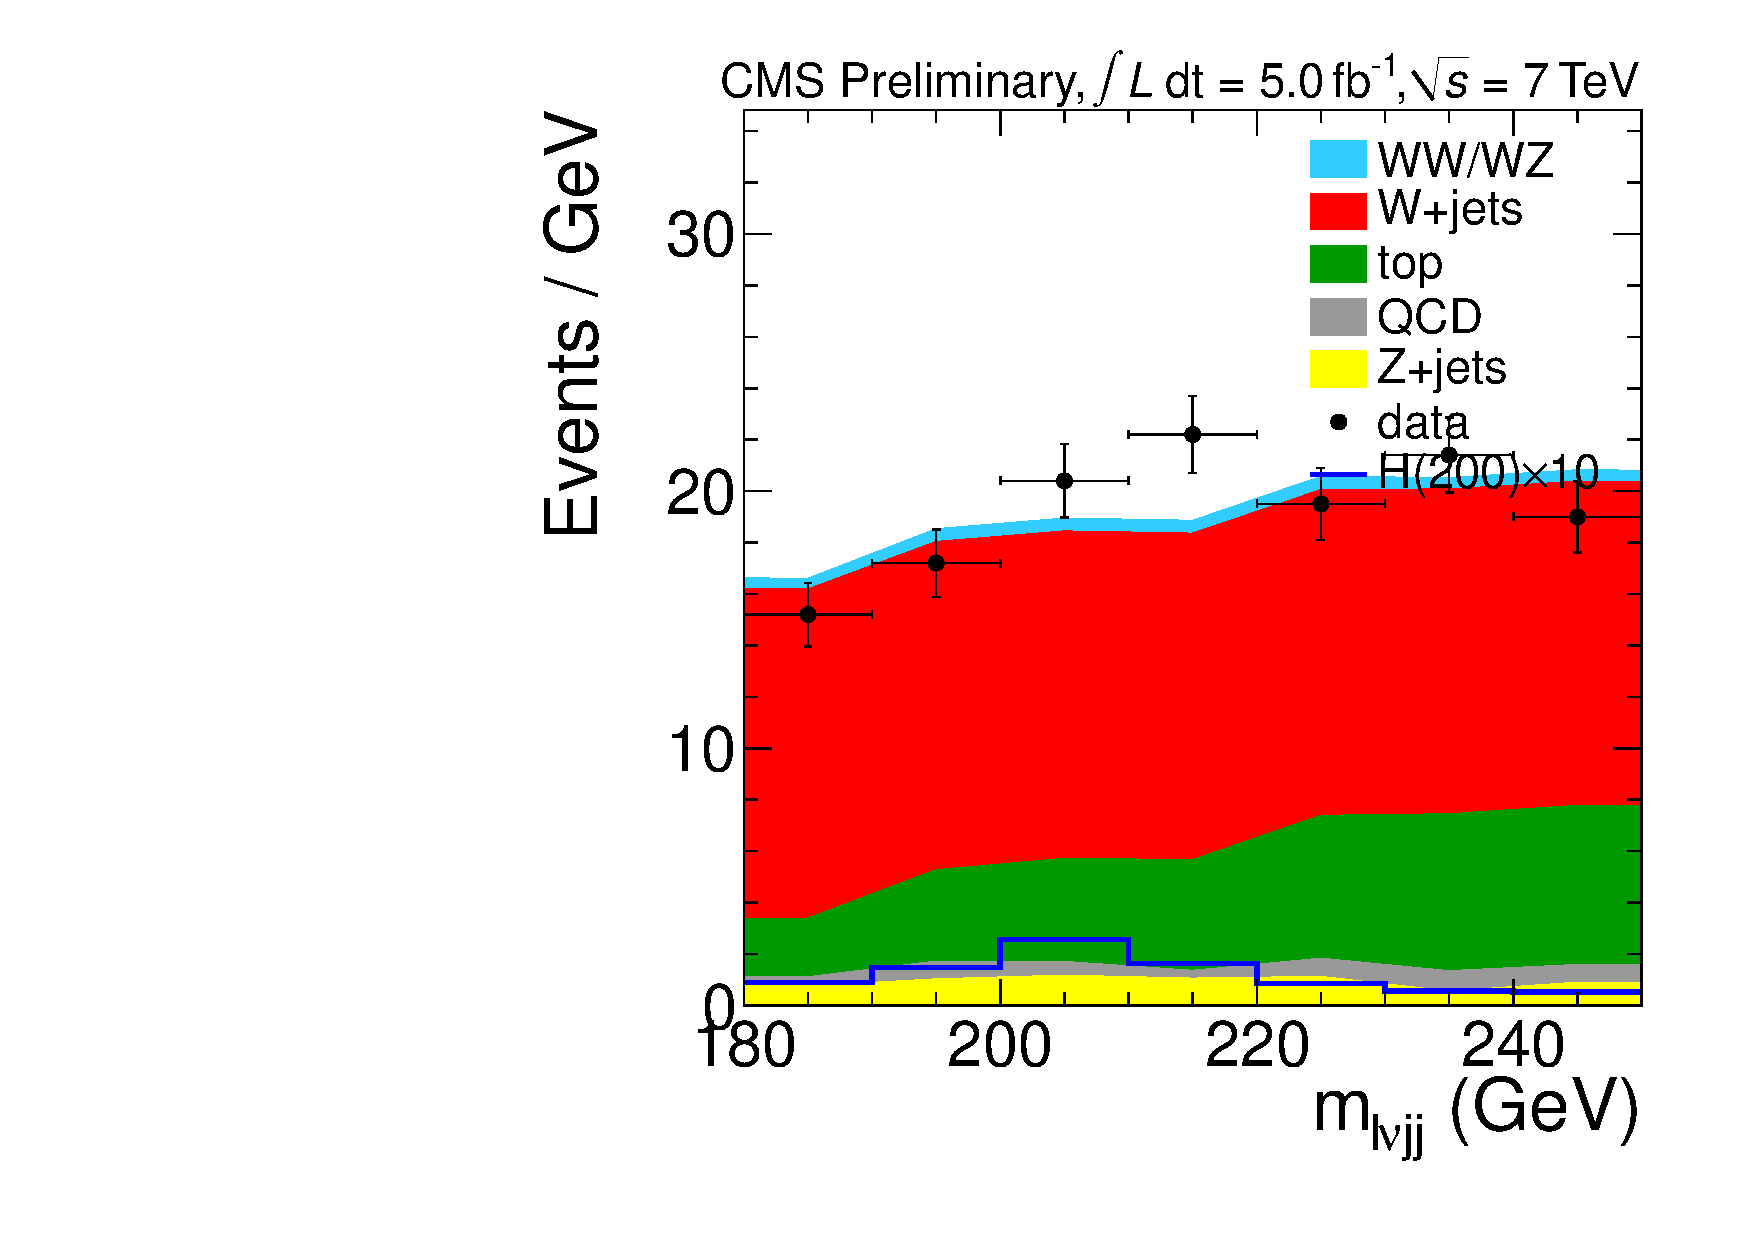
\includegraphics[width=0.3\textwidth]{plots/2012_FOURBSHAPES/H200_Mlvjj_Electron_3jets_Stacked}
% }
% \subfigure[]{
%   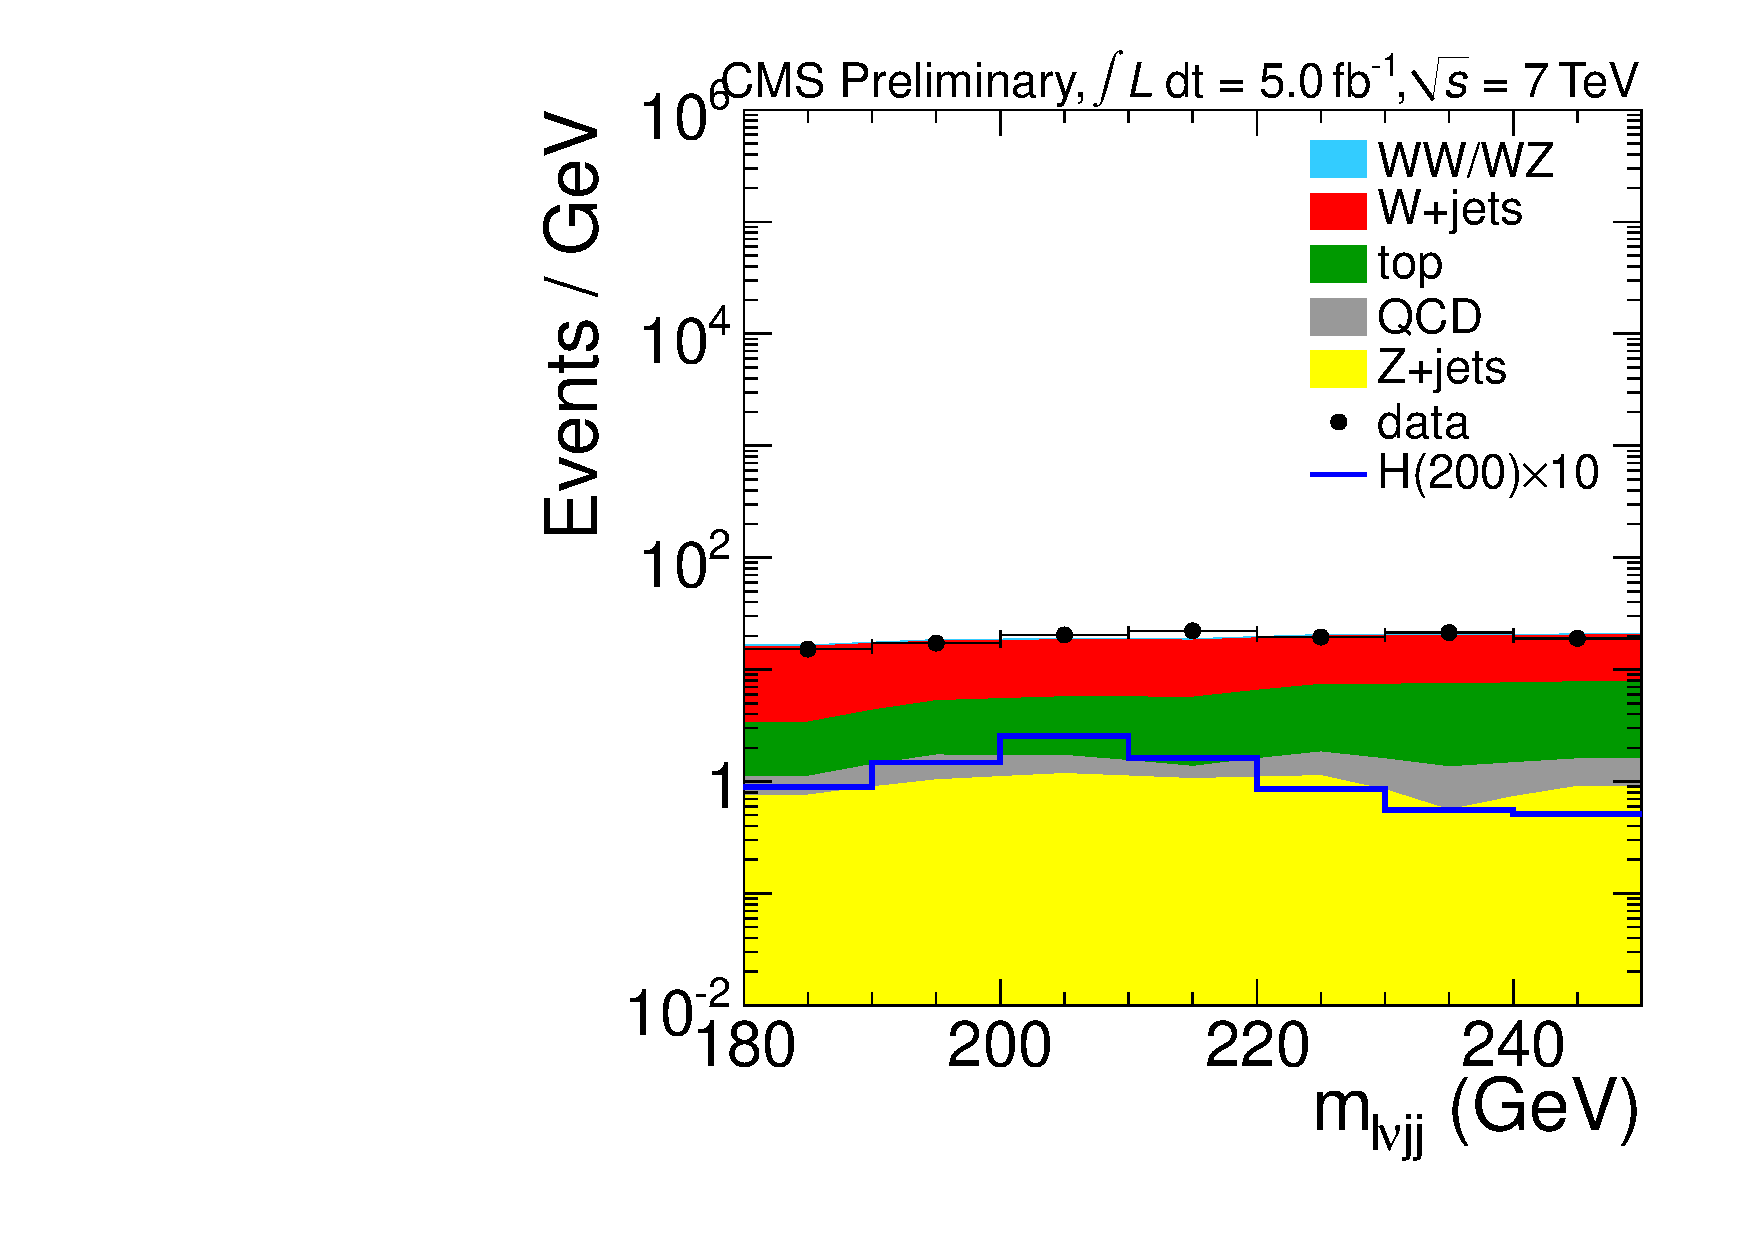
\includegraphics[width=0.3\textwidth]{plots/2012_FOURBSHAPES/H200_Mlvjj_Electron_3jets_Stacked_log}
% }
% \subfigure[]{
%   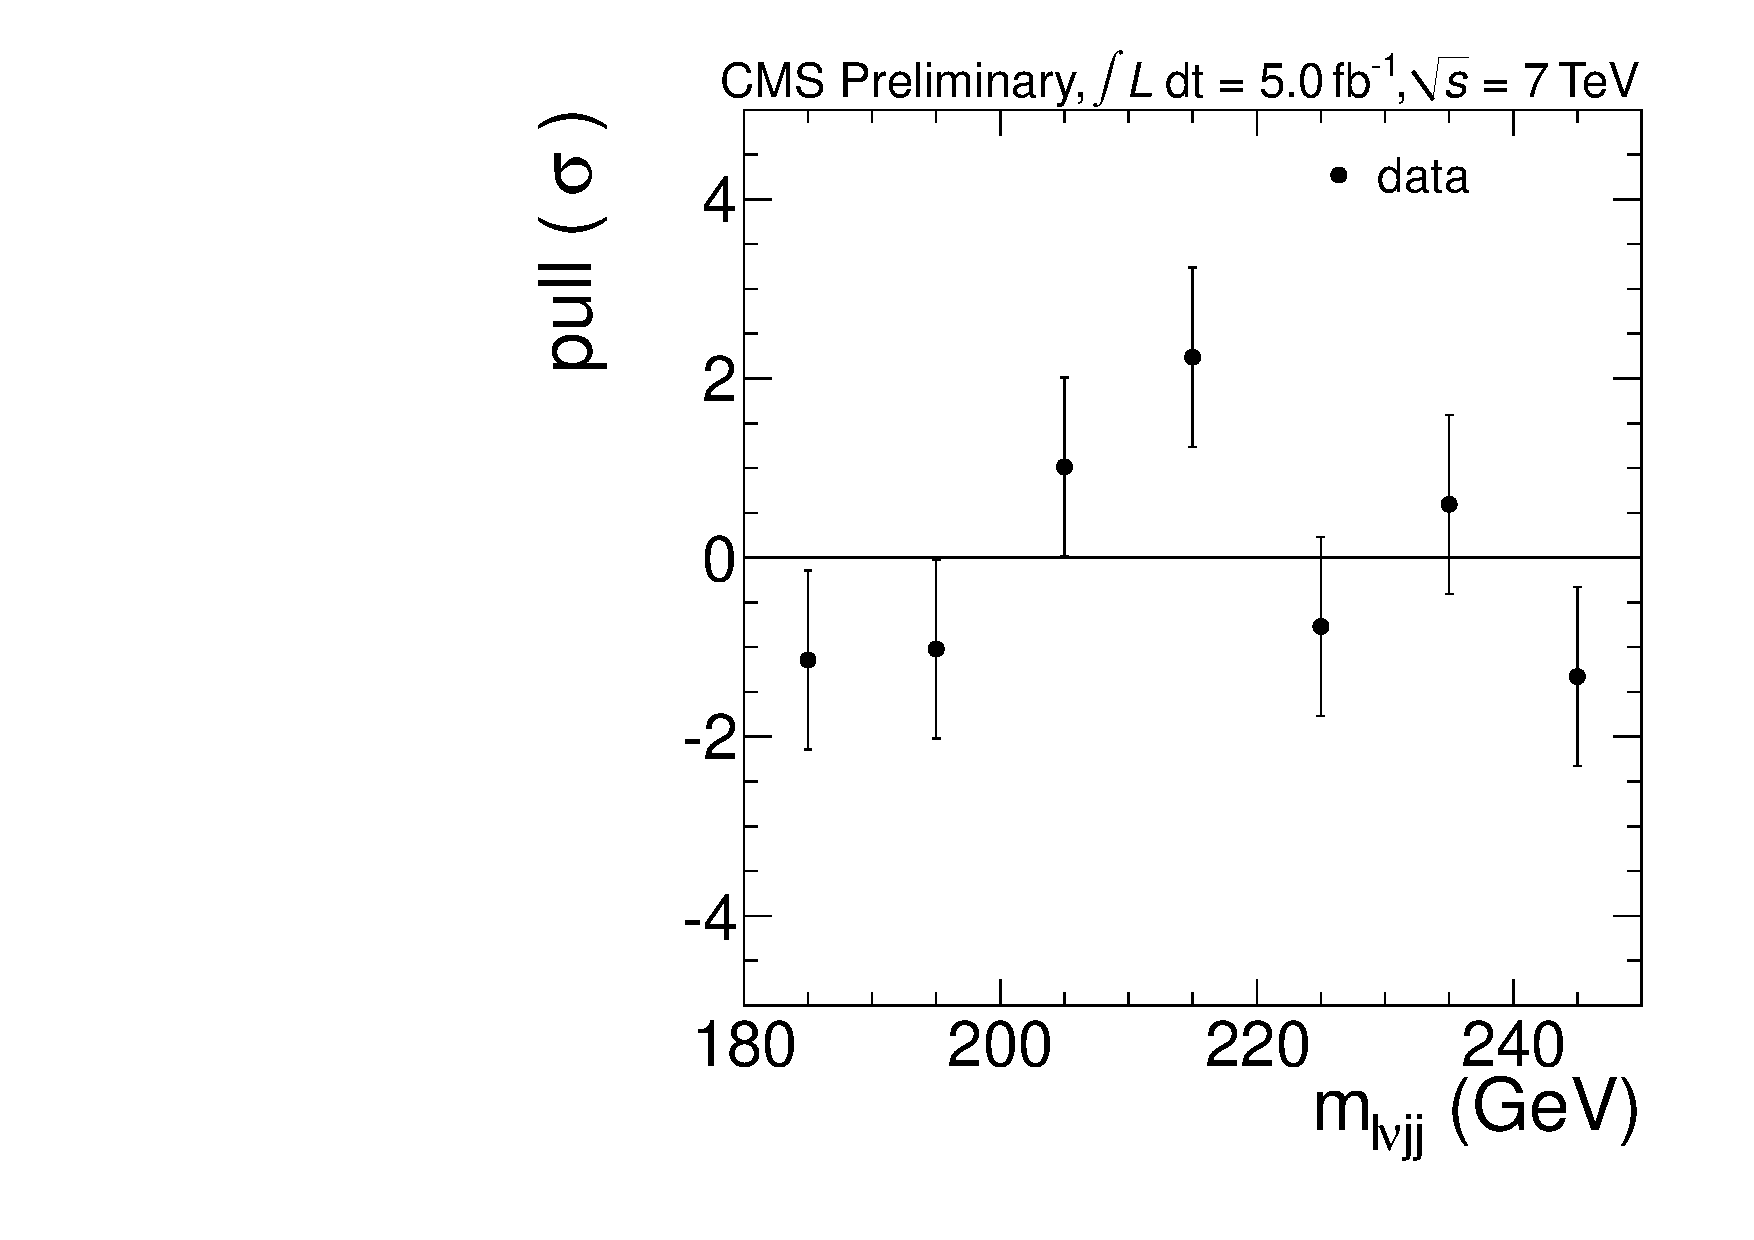
\includegraphics[width=0.3\textwidth]{plots/2012_FOURBSHAPES/H200_Mlvjj_Electron_3jets_Pull}
% }
% \caption{$M_H = 200$~GeV point. The distribution of the 4-body invariant mass $m_{\ell\nu jj}$ plotted on 
% linear (left) and log (center) scales. The pull distribution computed as 
% [(Data - Background)/ Background uncertainty] is shown on the right.
% The four rows correspond to muon 2-jets, muon 3-jets, electron 2-jets, 
% and electron 3-jets event categories, respectively. }
% \label{fig:mlnujj_mH200}
% \end{figure}
%%%%%%%%%%%%%%%%%%%%
%%%%%%%%%%%%%%%%%%%%
%%%%%%%%%%%%%%%%%%%%

% \begin{figure}[h!t]
% \subfigure[]{
%     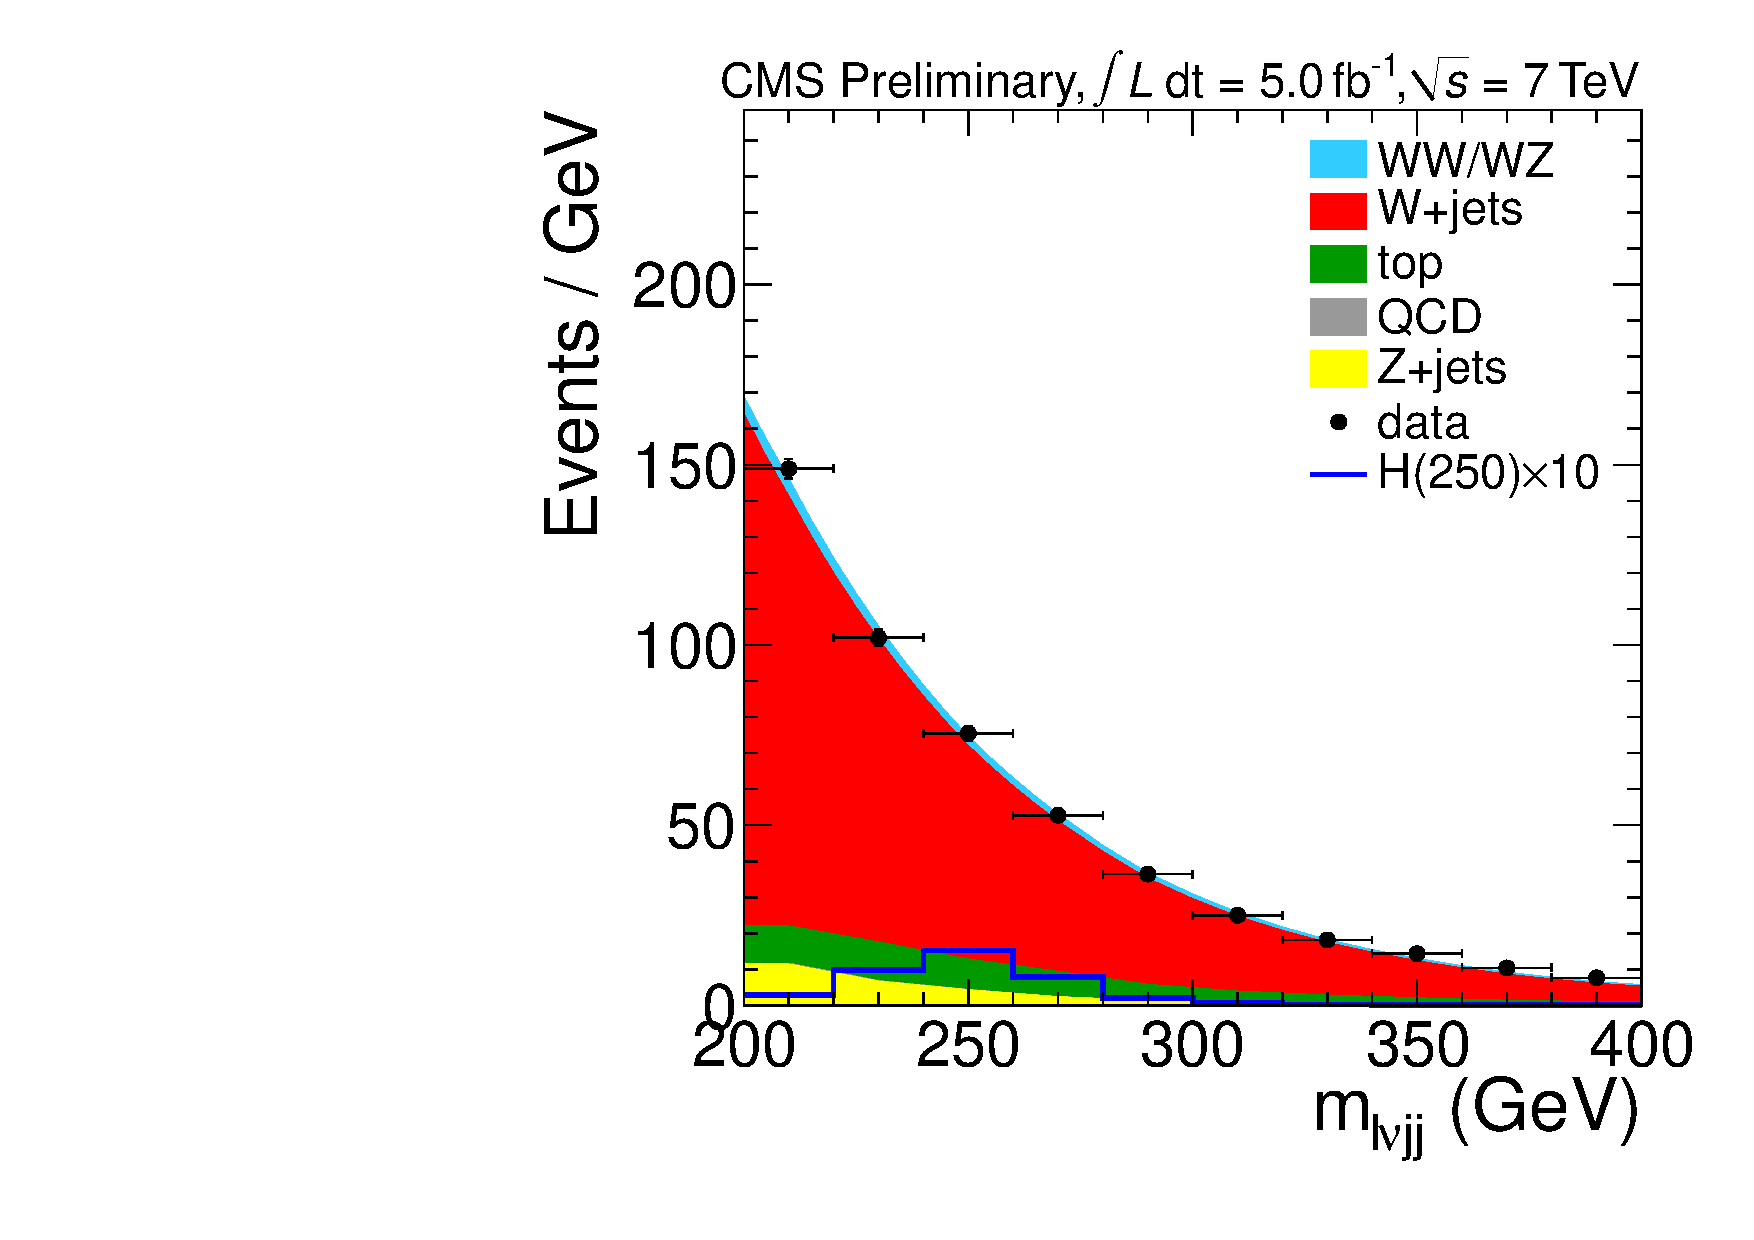
\includegraphics[width=0.3\textwidth]{plots/2012_FOURBSHAPES/H250_Mlvjj_Muon_2jets_Stacked}
% }
% \subfigure[]{
%   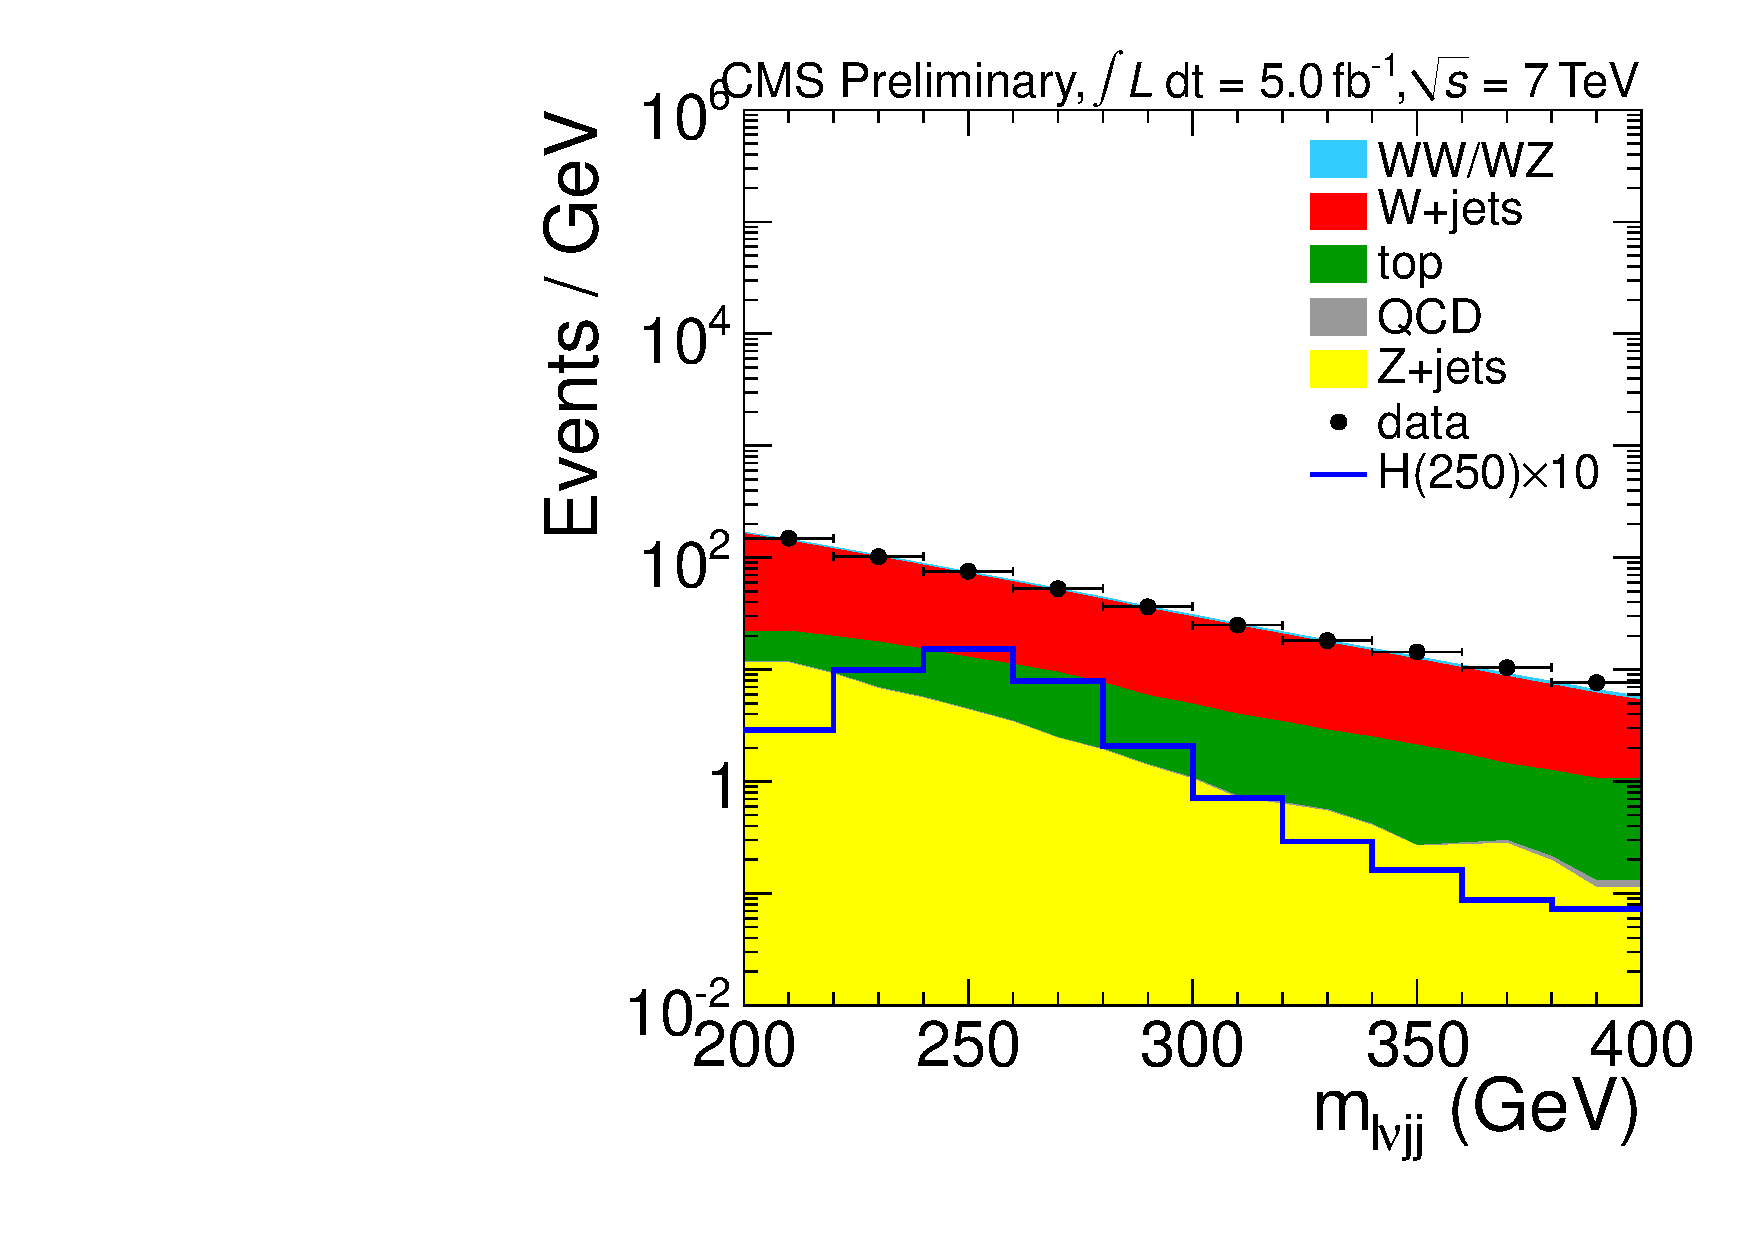
\includegraphics[width=0.3\textwidth]{plots/2012_FOURBSHAPES/H250_Mlvjj_Muon_2jets_Stacked_log}
% }
% \subfigure[]{
%   \includegraphics[width=0.3\textwidth]{plots/2012_FOURBSHAPES/H250_Mlvjj_Muon_2jets_Pull}
% }
% \vspace*{1mm} \\
% \subfigure[]{
%     \includegraphics[width=0.3\textwidth]{plots/2012_FOURBSHAPES/H250_Mlvjj_Muon_3jets_Stacked}
% }
% \subfigure[]{
%   \includegraphics[width=0.3\textwidth]{plots/2012_FOURBSHAPES/H250_Mlvjj_Muon_3jets_Stacked_log}
% }
% \subfigure[]{
%   \includegraphics[width=0.3\textwidth]{plots/2012_FOURBSHAPES/H250_Mlvjj_Muon_3jets_Pull}
% }
% \vspace*{1mm} \\
% \subfigure[]{
%     \includegraphics[width=0.3\textwidth]{plots/2012_FOURBSHAPES/H250_Mlvjj_Electron_2jets_Stacked}
% }
% \subfigure[]{
%   \includegraphics[width=0.3\textwidth]{plots/2012_FOURBSHAPES/H250_Mlvjj_Electron_2jets_Stacked_log}
% }
% \subfigure[]{
%   \includegraphics[width=0.3\textwidth]{plots/2012_FOURBSHAPES/H250_Mlvjj_Electron_2jets_Pull}
% }
% \vspace*{1mm} \\
% \subfigure[]{
%     \includegraphics[width=0.3\textwidth]{plots/2012_FOURBSHAPES/H250_Mlvjj_Electron_3jets_Stacked}
% }
% \subfigure[]{
%   \includegraphics[width=0.3\textwidth]{plots/2012_FOURBSHAPES/H250_Mlvjj_Electron_3jets_Stacked_log}
% }
% \subfigure[]{
%   \includegraphics[width=0.3\textwidth]{plots/2012_FOURBSHAPES/H250_Mlvjj_Electron_3jets_Pull}
% }
% \caption{$M_H = 250$~GeV point. The distribution of the 4-body invariant mass $m_{\ell\nu jj}$ plotted on 
% linear (left) and log (center) scales. The pull distribution computed as 
% [(Data - Background)/ Background uncertainty] is shown on the right.
% The four rows correspond to muon 2-jets, muon 3-jets, electron 2-jets, 
% and electron 3-jets event categories, respectively. }
% \label{fig:mlnujj_mH250}
% \end{figure}


%   %%%%%%%%%%%%%%%%%%%%
%   %%%%%%%%%%%%%%%%%%%%
%   %%%%%%%%%%%%%%%%%%%%
%  \begin{figure}[h!t]
%  \subfigure[]{
%      \includegraphics[width=0.3\textwidth]{plots/2012_FOURBSHAPES/H300_Mlvjj_Muon_2jets_Stacked}
%  }
%  \subfigure[]{
%    \includegraphics[width=0.3\textwidth]{plots/2012_FOURBSHAPES/H300_Mlvjj_Muon_2jets_Stacked_log}
%  }
%  \subfigure[]{
%    \includegraphics[width=0.3\textwidth]{plots/2012_FOURBSHAPES/H300_Mlvjj_Muon_2jets_Pull}
%  }
%  \vspace*{1mm} \\
%  \subfigure[]{
%      \includegraphics[width=0.3\textwidth]{plots/2012_FOURBSHAPES/H300_Mlvjj_Muon_3jets_Stacked}
%  }
%  \subfigure[]{
%    \includegraphics[width=0.3\textwidth]{plots/2012_FOURBSHAPES/H300_Mlvjj_Muon_3jets_Stacked_log}
%  }
%  \subfigure[]{
%    \includegraphics[width=0.3\textwidth]{plots/2012_FOURBSHAPES/H300_Mlvjj_Muon_3jets_Pull}
%  }
%  \vspace*{1mm} \\
%  \subfigure[]{
%      \includegraphics[width=0.3\textwidth]{plots/2012_FOURBSHAPES/H300_Mlvjj_Electron_2jets_Stacked}
%  }
%  \subfigure[]{
%    \includegraphics[width=0.3\textwidth]{plots/2012_FOURBSHAPES/H300_Mlvjj_Electron_2jets_Stacked_log}
%  }
%  \subfigure[]{
%    \includegraphics[width=0.3\textwidth]{plots/2012_FOURBSHAPES/H300_Mlvjj_Electron_2jets_Pull}
%  }
%  \vspace*{1mm} \\
%  \subfigure[]{
%      \includegraphics[width=0.3\textwidth]{plots/2012_FOURBSHAPES/H300_Mlvjj_Electron_3jets_Stacked}
%  }
%  \subfigure[]{
%    \includegraphics[width=0.3\textwidth]{plots/2012_FOURBSHAPES/H300_Mlvjj_Electron_3jets_Stacked_log}
%  }
%  \subfigure[]{
%    \includegraphics[width=0.3\textwidth]{plots/2012_FOURBSHAPES/H300_Mlvjj_Electron_3jets_Pull}
%  }
%  \caption{$M_H = 300$~GeV point. The distribution of the 4-body invariant mass $m_{\ell\nu jj}$ plotted on 
%  linear (left) and log (center) scales. The pull distribution computed as 
%  [(Data - Background)/ Background uncertainty] is shown on the right.
%  The four rows correspond to muon 2-jets, muon 3-jets, electron 2-jets, 
%  and electron 3-jets event categories, respectively. }
%  \label{fig:mlnujj_mH300}
%  \end{figure}
%   %%%%%%%%%%%%%%%%%%%%
%   %%%%%%%%%%%%%%%%%%%%
%   %%%%%%%%%%%%%%%%%%%%
\begin{figure}[h!t]
\subfigure[]{
    \includegraphics[width=0.3\textwidth]{plots/2012_FOURBSHAPES/H350_Mlvjj_Muon_2jets_Stacked}
}
\subfigure[]{
  \includegraphics[width=0.3\textwidth]{plots/2012_FOURBSHAPES/H350_Mlvjj_Muon_2jets_Stacked_log}
}
\subfigure[]{
  \includegraphics[width=0.3\textwidth]{plots/2012_FOURBSHAPES/H350_Mlvjj_Muon_2jets_Pull}
}
\vspace*{1mm} \\
\subfigure[]{
    \includegraphics[width=0.3\textwidth]{plots/2012_FOURBSHAPES/H350_Mlvjj_Muon_3jets_Stacked}
}
\subfigure[]{
  \includegraphics[width=0.3\textwidth]{plots/2012_FOURBSHAPES/H350_Mlvjj_Muon_3jets_Stacked_log}
}
\subfigure[]{
  \includegraphics[width=0.3\textwidth]{plots/2012_FOURBSHAPES/H350_Mlvjj_Muon_3jets_Pull}
}
\vspace*{1mm} \\
\subfigure[]{
    \includegraphics[width=0.3\textwidth]{plots/2012_FOURBSHAPES/H350_Mlvjj_Electron_2jets_Stacked}
}
\subfigure[]{
  \includegraphics[width=0.3\textwidth]{plots/2012_FOURBSHAPES/H350_Mlvjj_Electron_2jets_Stacked_log}
}
\subfigure[]{
  \includegraphics[width=0.3\textwidth]{plots/2012_FOURBSHAPES/H350_Mlvjj_Electron_2jets_Pull}
}
\vspace*{1mm} \\
\subfigure[]{
    \includegraphics[width=0.3\textwidth]{plots/2012_FOURBSHAPES/H350_Mlvjj_Electron_3jets_Stacked}
}
\subfigure[]{
  \includegraphics[width=0.3\textwidth]{plots/2012_FOURBSHAPES/H350_Mlvjj_Electron_3jets_Stacked_log}
}
\subfigure[]{
  \includegraphics[width=0.3\textwidth]{plots/2012_FOURBSHAPES/H350_Mlvjj_Electron_3jets_Pull}
}
\caption{$M_H = 350$~GeV point. The distribution of the 4-body invariant mass $m_{\ell\nu jj}$ plotted on 
linear (left) and log (center) scales. The pull distribution computed as 
[(Data - Background)/ Background uncertainty] is shown on the right.
The four rows correspond to muon 2-jets, muon 3-jets, electron 2-jets, 
and electron 3-jets event categories, respectively. }
\label{fig:mlnujj_mH350}
\end{figure}
%   %%%%%%%%%%%%%%%%%%%%
%   %%%%%%%%%%%%%%%%%%%%
%   %%%%%%%%%%%%%%%%%%%%
%\begin{figure}[h!t]
%  \subfigure[]{
%      \includegraphics[width=0.3\textwidth]{plots/2012_FOURBSHAPES/H400_Mlvjj_Muon_2jets_Stacked}
%  }
%  \subfigure[]{
%    \includegraphics[width=0.3\textwidth]{plots/2012_FOURBSHAPES/H400_Mlvjj_Muon_2jets_Stacked_log}
%  }
%  \subfigure[]{
%    \includegraphics[width=0.3\textwidth]{plots/2012_FOURBSHAPES/H400_Mlvjj_Muon_2jets_Pull}
%  }
%  \vspace*{1mm} \\
%  \subfigure[]{
%      \includegraphics[width=0.3\textwidth]{plots/2012_FOURBSHAPES/H400_Mlvjj_Muon_3jets_Stacked}
%  }
%  \subfigure[]{
%    \includegraphics[width=0.3\textwidth]{plots/2012_FOURBSHAPES/H400_Mlvjj_Muon_3jets_Stacked_log}
%  }
%  \subfigure[]{
%    \includegraphics[width=0.3\textwidth]{plots/2012_FOURBSHAPES/H400_Mlvjj_Muon_3jets_Pull}
%  }
%  \vspace*{1mm} \\
%  \subfigure[]{
%      \includegraphics[width=0.3\textwidth]{plots/2012_FOURBSHAPES/H400_Mlvjj_Electron_2jets_Stacked}
%  }
%  \subfigure[]{
%    \includegraphics[width=0.3\textwidth]{plots/2012_FOURBSHAPES/H400_Mlvjj_Electron_2jets_Stacked_log}
%  }
%  \subfigure[]{
%    \includegraphics[width=0.3\textwidth]{plots/2012_FOURBSHAPES/H400_Mlvjj_Electron_2jets_Pull}
%  }
%  \vspace*{1mm} \\
%  \subfigure[]{
%      \includegraphics[width=0.3\textwidth]{plots/2012_FOURBSHAPES/H400_Mlvjj_Electron_3jets_Stacked}
%  }
%  \subfigure[]{
%    \includegraphics[width=0.3\textwidth]{plots/2012_FOURBSHAPES/H400_Mlvjj_Electron_3jets_Stacked_log}
%  }
%  \subfigure[]{
%    \includegraphics[width=0.3\textwidth]{plots/2012_FOURBSHAPES/H400_Mlvjj_Electron_3jets_Pull}
%  }
%  \caption{$M_H = 400$~GeV point. The distribution of the 4-body invariant mass $m_{\ell\nu jj}$ plotted on 
%           linear (left) and log (center) scales. The pull distribution computed as 
%           [(Data - Background)/ Background uncertainty] is shown on the right.
%           The four rows correspond to muon 2-jets, muon 3-jets, electron 2-jets, 
%           and electron 3-jets event categories, respectively. }
%  \label{fig:mlnujj_mH400}
%\end{figure}
%   %%%%%%%%%%%%%%%%%%%%
%   %%%%%%%%%%%%%%%%%%%%
%   %%%%%%%%%%%%%%%%%%%%
\begin{figure}[h!t]
\subfigure[]{
    \includegraphics[width=0.3\textwidth]{plots/2012_FOURBSHAPES/H450_Mlvjj_Muon_2jets_Stacked}
}
\subfigure[]{
  \includegraphics[width=0.3\textwidth]{plots/2012_FOURBSHAPES/H450_Mlvjj_Muon_2jets_Stacked_log}
}
\subfigure[]{
  \includegraphics[width=0.3\textwidth]{plots/2012_FOURBSHAPES/H450_Mlvjj_Muon_2jets_Pull}
}
\vspace*{1mm} \\
\subfigure[]{
    \includegraphics[width=0.3\textwidth]{plots/2012_FOURBSHAPES/H450_Mlvjj_Muon_3jets_Stacked}
}
\subfigure[]{
  \includegraphics[width=0.3\textwidth]{plots/2012_FOURBSHAPES/H450_Mlvjj_Muon_3jets_Stacked_log}
}
\subfigure[]{
  \includegraphics[width=0.3\textwidth]{plots/2012_FOURBSHAPES/H450_Mlvjj_Muon_3jets_Pull}
}
\vspace*{1mm} \\
\subfigure[]{
    \includegraphics[width=0.3\textwidth]{plots/2012_FOURBSHAPES/H450_Mlvjj_Electron_2jets_Stacked}
}
\subfigure[]{
  \includegraphics[width=0.3\textwidth]{plots/2012_FOURBSHAPES/H450_Mlvjj_Electron_2jets_Stacked_log}
}
\subfigure[]{
  \includegraphics[width=0.3\textwidth]{plots/2012_FOURBSHAPES/H450_Mlvjj_Electron_2jets_Pull}
}
\vspace*{1mm} \\
\subfigure[]{
    \includegraphics[width=0.3\textwidth]{plots/2012_FOURBSHAPES/H450_Mlvjj_Electron_3jets_Stacked}
}
\subfigure[]{
  \includegraphics[width=0.3\textwidth]{plots/2012_FOURBSHAPES/H450_Mlvjj_Electron_3jets_Stacked_log}
}
\subfigure[]{
  \includegraphics[width=0.3\textwidth]{plots/2012_FOURBSHAPES/H450_Mlvjj_Electron_3jets_Pull}
}
\caption{$M_H = 450$~GeV point. The distribution of the 4-body invariant mass $m_{\ell\nu jj}$ plotted on 
linear (left) and log (center) scales. The pull distribution computed as 
[(Data - Background)/ Background uncertainty] is shown on the right.
The four rows correspond to muon 2-jets, muon 3-jets, electron 2-jets, 
and electron 3-jets event categories, respectively. }
\label{fig:mlnujj_mH450}
\end{figure}
%   %%%%%%%%%%%%%%%%%%%%
%   %%%%%%%%%%%%%%%%%%%%
%   %%%%%%%%%%%%%%%%%%%%
\begin{figure}[h!t]
\subfigure[]{
    \includegraphics[width=0.3\textwidth]{plots/2012_FOURBSHAPES/H500_Mlvjj_Muon_2jets_Stacked}
}
\subfigure[]{
  \includegraphics[width=0.3\textwidth]{plots/2012_FOURBSHAPES/H500_Mlvjj_Muon_2jets_Stacked_log}
}
\subfigure[]{
  \includegraphics[width=0.3\textwidth]{plots/2012_FOURBSHAPES/H500_Mlvjj_Muon_2jets_Pull}
}
\vspace*{1mm} \\
\subfigure[]{
    \includegraphics[width=0.3\textwidth]{plots/2012_FOURBSHAPES/H500_Mlvjj_Muon_3jets_Stacked}
}
\subfigure[]{
  \includegraphics[width=0.3\textwidth]{plots/2012_FOURBSHAPES/H500_Mlvjj_Muon_3jets_Stacked_log}
}
\subfigure[]{
  \includegraphics[width=0.3\textwidth]{plots/2012_FOURBSHAPES/H500_Mlvjj_Muon_3jets_Pull}
}
\vspace*{1mm} \\
\subfigure[]{
    \includegraphics[width=0.3\textwidth]{plots/2012_FOURBSHAPES/H500_Mlvjj_Electron_2jets_Stacked}
}
\subfigure[]{
  \includegraphics[width=0.3\textwidth]{plots/2012_FOURBSHAPES/H500_Mlvjj_Electron_2jets_Stacked_log}
}
\subfigure[]{
  \includegraphics[width=0.3\textwidth]{plots/2012_FOURBSHAPES/H500_Mlvjj_Electron_2jets_Pull}
}
\vspace*{1mm} \\
\subfigure[]{
    \includegraphics[width=0.3\textwidth]{plots/2012_FOURBSHAPES/H500_Mlvjj_Electron_3jets_Stacked}
}
\subfigure[]{
  \includegraphics[width=0.3\textwidth]{plots/2012_FOURBSHAPES/H500_Mlvjj_Electron_3jets_Stacked_log}
}
\subfigure[]{
  \includegraphics[width=0.3\textwidth]{plots/2012_FOURBSHAPES/H500_Mlvjj_Electron_3jets_Pull}
}
\caption{$M_H = 500$~GeV point. The distribution of the 4-body invariant mass $m_{\ell\nu jj}$ plotted on 
linear (left) and log (center) scales. The pull distribution computed as 
[(Data - Background)/ Background uncertainty] is shown on the right.
The four rows correspond to muon 2-jets, muon 3-jets, electron 2-jets, 
and electron 3-jets event categories, respectively. }
\label{fig:mlnujj_mH500}
\end{figure}
%   %%%%%%%%%%%%%%%%%%%%
%   %%%%%%%%%%%%%%%%%%%%
%   %%%%%%%%%%%%%%%%%%%%
% \begin{figure}[h!t]
% \subfigure[]{
%     \includegraphics[width=0.3\textwidth]{plots/2012_FOURBSHAPES/H550_Mlvjj_Muon_2jets_Stacked}
% }
% \subfigure[]{
%   \includegraphics[width=0.3\textwidth]{plots/2012_FOURBSHAPES/H550_Mlvjj_Muon_2jets_Stacked_log}
% }
% \subfigure[]{
%   \includegraphics[width=0.3\textwidth]{plots/2012_FOURBSHAPES/H550_Mlvjj_Muon_2jets_Pull}
% }
% \vspace*{1mm} \\
% \subfigure[]{
%     \includegraphics[width=0.3\textwidth]{plots/2012_FOURBSHAPES/H550_Mlvjj_Muon_3jets_Stacked}
% }
% \subfigure[]{
%   \includegraphics[width=0.3\textwidth]{plots/2012_FOURBSHAPES/H550_Mlvjj_Muon_3jets_Stacked_log}
% }
% \subfigure[]{
%   \includegraphics[width=0.3\textwidth]{plots/2012_FOURBSHAPES/H550_Mlvjj_Muon_3jets_Pull}
% }
% \vspace*{1mm} \\
% \subfigure[]{
%     \includegraphics[width=0.3\textwidth]{plots/2012_FOURBSHAPES/H550_Mlvjj_Electron_2jets_Stacked}
% }
% \subfigure[]{
%   \includegraphics[width=0.3\textwidth]{plots/2012_FOURBSHAPES/H550_Mlvjj_Electron_2jets_Stacked_log}
% }
% \subfigure[]{
%   \includegraphics[width=0.3\textwidth]{plots/2012_FOURBSHAPES/H550_Mlvjj_Electron_2jets_Pull}
% }
% \vspace*{1mm} \\
% \subfigure[]{
%     \includegraphics[width=0.3\textwidth]{plots/2012_FOURBSHAPES/H550_Mlvjj_Electron_3jets_Stacked}
% }
% \subfigure[]{
%   \includegraphics[width=0.3\textwidth]{plots/2012_FOURBSHAPES/H550_Mlvjj_Electron_3jets_Stacked_log}
% }
% \subfigure[]{
%   \includegraphics[width=0.3\textwidth]{plots/2012_FOURBSHAPES/H550_Mlvjj_Electron_3jets_Pull}
% }
% \caption{$M_H = 550$~GeV point. The distribution of the 4-body invariant mass $m_{\ell\nu jj}$ plotted on 
% linear (left) and log (center) scales. The pull distribution computed as 
% [(Data - Background)/ Background uncertainty] is shown on the right.
% The four rows correspond to muon 2-jets, muon 3-jets, electron 2-jets, 
% and electron 3-jets event categories, respectively. }
% \label{fig:mlnujj_mH550}
% \end{figure}
%   %%%%%%%%%%%%%%%%%%%%
%   %%%%%%%%%%%%%%%%%%%%
%   %%%%%%%%%%%%%%%%%%%%
\begin{figure}[h!t]
\subfigure[]{
    \includegraphics[width=0.3\textwidth]{plots/2012_FOURBSHAPES/H600_Mlvjj_Muon_2jets_Stacked}
}
\subfigure[]{
  \includegraphics[width=0.3\textwidth]{plots/2012_FOURBSHAPES/H600_Mlvjj_Muon_2jets_Stacked_log}
}
\subfigure[]{
  \includegraphics[width=0.3\textwidth]{plots/2012_FOURBSHAPES/H600_Mlvjj_Muon_2jets_Pull}
}
\vspace*{1mm} \\
\subfigure[]{
    \includegraphics[width=0.3\textwidth]{plots/2012_FOURBSHAPES/H600_Mlvjj_Muon_3jets_Stacked}
}
\subfigure[]{
  \includegraphics[width=0.3\textwidth]{plots/2012_FOURBSHAPES/H600_Mlvjj_Muon_3jets_Stacked_log}
}
\subfigure[]{
  \includegraphics[width=0.3\textwidth]{plots/2012_FOURBSHAPES/H600_Mlvjj_Muon_3jets_Pull}
}
\vspace*{1mm} \\
\subfigure[]{
    \includegraphics[width=0.3\textwidth]{plots/2012_FOURBSHAPES/H600_Mlvjj_Electron_2jets_Stacked}
}
\subfigure[]{
  \includegraphics[width=0.3\textwidth]{plots/2012_FOURBSHAPES/H600_Mlvjj_Electron_2jets_Stacked_log}
}
\subfigure[]{
  \includegraphics[width=0.3\textwidth]{plots/2012_FOURBSHAPES/H600_Mlvjj_Electron_2jets_Pull}
}
\vspace*{1mm} \\
\subfigure[]{
    \includegraphics[width=0.3\textwidth]{plots/2012_FOURBSHAPES/H600_Mlvjj_Electron_3jets_Stacked}
}
\subfigure[]{
  \includegraphics[width=0.3\textwidth]{plots/2012_FOURBSHAPES/H600_Mlvjj_Electron_3jets_Stacked_log}
}
\subfigure[]{
  \includegraphics[width=0.3\textwidth]{plots/2012_FOURBSHAPES/H600_Mlvjj_Electron_3jets_Pull}
}
\caption{$M_H = 600$~GeV point. The distribution of the 4-body invariant mass $m_{\ell\nu jj}$ plotted on 
linear (left) and log (center) scales. The pull distribution computed as 
[(Data - Background)/ Background uncertainty] is shown on the right.
The four rows correspond to muon 2-jets, muon 3-jets, electron 2-jets, 
and electron 3-jets event categories, respectively. }
\label{fig:mlnujj_mH600}
\end{figure}
